% !TeX program = lualatex
\documentclass[12pt,oneside,a4paper,brazil,chapter=TITLE]{abntex2}
\usepackage{fontspec}
% Compilar com LuaLaTeX; Arial deve estar instalada no sistema.
% O modelo admite Arial nos elementos iniciais, mas solicita Times no corpo.
% Manter compilação disponível enquanto Times New Roman não estiver instalada.
\IfFontExistsTF{Times New Roman}{\setmainfont{Times New Roman}}{\setmainfont{Arial}}
\setsansfont{Arial}
\usepackage{microtype,indentfirst,graphicx,url,enumitem,float,xcolor}
\newcommand{\pendente}[1]{\textbf{\textcolor{red!65!black}{[PENDENTE: #1]}}}
\usepackage{longtable,array,amsmath,xurl,tikz}
\usetikzlibrary{arrows.meta,shapes.geometric,positioning}
% Autor-data conforme os exemplos da Live da Quinzena 4.
\usepackage[authoryear,round]{natbib}
\setcitestyle{aysep={,},citesep={;}}
% Datas estimadas podem conter colchetes e não cabem no analisador de quatro
% caracteres do natbib. Preservar a data inteira, também nas citações múltiplas.
\makeatletter
\def\NAT@parse@date#1@@{\let\NAT@year\NAT@date\let\NAT@exlab\NAT@date}
\makeatother
\setlength{\bibhang}{0pt}
\setlength{\bibsep}{\baselineskip}
\usepackage{hyperref}
\hypersetup{hypertexnames=false,hidelinks}
\graphicspath{{imgs/}}
% Numeração no alto à direita, inclusive nas aberturas de capítulos.
\makepagestyle{papnumeracao}
\makeoddhead{papnumeracao}{}{}{\ABNTEXfontereduzida\thepage}
\makeevenhead{papnumeracao}{}{}{\ABNTEXfontereduzida\thepage}

\titulo{Sistema de acesso a informações do transporte público por QR Code em pontos de ônibus}
\autor{André Meneghelli Vale \\ Ariana Harumi Uemura \\ Bruno Gabriel Migliari de Souza \\ Caio Wellington Procopio Ferreira \\ Ingrid Emanuelle Sousa Dias \\ Leonardo Souza Leite \\ Maurício Gonçalves Marques \\ Nathalia Almeida Amorim}
\local{São Bernardo do Campo; Suzano; Francisco Morato; Osasco -- SP}
\data{2026}
\instituicao{Universidade Virtual do Estado de São Paulo -- UNIVESP}
\tipotrabalho{Relatório Técnico-Científico Final}
\preambulo{Relatório Técnico-Científico apresentado na disciplina de Projeto Integrador em Computação II, para o curso de Bacharelado em Tecnologia da Informação da Universidade Virtual do Estado de São Paulo (UNIVESP).}
\orientador[Facilitadora:]{Me. Aline Monteiro Campos Garcia}
% Logotipo oficial apenas na capa; imagens compartilhadas em docs/imagens.
\renewcommand{\imprimircapa}{%
  \begin{capa}
    \centering
    \includegraphics[width=5cm,keepaspectratio]{Univesp_logo_png_rgb.png}\par
    \vspace{0.6cm}
    {\normalfont\fontsize{14}{17}\selectfont\imprimirinstituicao\par}
    \vspace{1cm}
    {\normalfont\fontsize{14}{17}\selectfont\imprimirautor\par}
    \vfill
    {\normalfont\bfseries\fontsize{14}{17}\selectfont\imprimirtitulo\par}
    \vfill
    {\normalsize Vídeo de apresentação do Projeto Integrador: \pendente{inserir link}.\par}
    \vspace{0.6cm}
    {\large\imprimirlocal\par}
    {\large\imprimirdata\par}
    \vspace*{1cm}
  \end{capa}
}
\setlrmarginsandblock{3cm}{2cm}{*}
\setulmarginsandblock{3cm}{2cm}{*}
\checkandfixthelayout
\setlength{\parskip}{\baselineskip}
\setlength{\beforesecskip}{0pt}
\let\papsection\section
\renewcommand{\section}{\clearpage\papsection}
\let\papsubsection\subsection
\renewcommand{\subsection}{\clearpage\papsubsection}
\renewcommand{\ABNTEXchapterfont}{\normalfont\bfseries}
\renewcommand{\ABNTEXchapterfontsize}{\normalsize}
\begin{document}
\selectlanguage{brazil}\frenchspacing
\imprimircapa
\pretextual
% A capa fica fora da contagem; a folha de rosto inicia a sequência.
\pagenumbering{arabic}
\begin{folhaderosto}
\centering
{\fontsize{14}{17}\selectfont UNIVERSIDADE VIRTUAL DO ESTADO DE SÃO PAULO\par}
\vfill
{\fontsize{14}{17}\selectfont\bfseries\imprimirtitulo\par}
\vfill
\begin{flushright}
\begin{minipage}{0.58\textwidth}
\SingleSpacing\imprimirpreambulo\par
Facilitadora: Me. Aline Monteiro Campos Garcia.\par
Polos: São Bernardo do Campo; Suzano; Francisco Morato; Osasco -- SP.
\end{minipage}
\end{flushright}
\vfill
\imprimirlocal\par\imprimirdata
\end{folhaderosto}
\begin{resumo}
\SingleSpacing
\noindent VALE, André Meneghelli; UEMURA, Ariana Harumi; SOUZA, Bruno Gabriel Migliari de; FERREIRA, Caio Wellington Procopio; DIAS, Ingrid Emanuelle Sousa; LEITE, Leonardo Souza; MARQUES, Maurício Gonçalves; AMORIM, Nathalia Almeida. \textit{\imprimirtitulo}. \pendente{conferir total de folhas na versão de entrega}. Relatório Técnico-Científico. Bacharelado em Tecnologia da Informação -- Universidade Virtual do Estado de São Paulo. Facilitadora: Me. Aline Monteiro Campos Garcia. Polos: São Bernardo do Campo; Suzano; Francisco Morato; Osasco -- SP. 2026.
\par\medskip
Este trabalho apresenta o Ponto a Ponto (PaP), protótipo web de informação ao passageiro desenvolvido no Projeto Integrador em Computação II da UNIVESP. O objetivo é reduzir o esforço de interação necessário para consultar e escolher um deslocamento, identificando a origem por QR Code no ponto de ônibus e permitindo informar o destino sem conhecimento prévio das linhas. A metodologia reúne interlocução com a gestão do transporte de Mauá, pesquisa bibliográfica, análise de serviços existentes, prototipação e verificação técnica, organizadas pelas etapas do Design Thinking. A fundamentação de Interação Humano--Computador orienta a redução de etapas desnecessárias, o reconhecimento das opções e o feedback das ações. A aplicação utiliza Django, React e SQLite. O cenário histórico de Mauá emprega dados cadastrais e operação simulada; a solução final de São Paulo utiliza GTFS e integração com a API Olho Vivo para consultar previsões e posições quando esses dados estão disponíveis para a linha e a parada correspondentes. O planejamento dessa extensão considera horários programados, espera, caminhadas e baldeações, com busca limitada por rodadas. Os resultados incluem acesso contextualizado, favoritos, comparação de alternativas e visualização dos trechos no mapa. A avaliação com passageiros permanece pendente; os testes técnicos não demonstram melhoria de usabilidade ou precisão operacional. Conclui-se que o protótipo oferece uma base para avaliar a continuidade entre identificação da parada e escolha do percurso, condicionada à qualidade dos dados e à futura verificação com a comunidade.

\par\vfill
\noindent\textbf{Palavras-chave}: transporte público; QR Code; informação ao passageiro; mobilidade urbana; pontos de interesse.
\end{resumo}
% Ajuste local do espaço do título; preserva fonte e entradas do sumário.
\begingroup
\SingleSpacing
\setlength{\beforechapskip}{0pt}
\setlength{\afterchapskip}{6pt}
\setlength{\cftbeforechapterskip}{2pt}
\setlength{\cftbeforesubsectionskip}{-1.8pt}
\tableofcontents*
\endgroup
\cleardoublepage

\textual
\OnehalfSpacing
\pagestyle{papnumeracao}
\aliaspagestyle{chapter}{papnumeracao}
\setcounter{page}{1}
\chapter{Introdução}
Para quem está em um ponto de ônibus, decidir como chegar ao destino envolve reconhecer a parada, identificar as linhas e compreender o sentido do percurso e as eventuais trocas. Este trabalho investiga como facilitar essas decisões no transporte público de Mauá, especialmente quando o passageiro não conhece previamente a rede. Desenvolvido no Projeto Integrador em Computação II da UNIVESP, articula conhecimentos de computação e interlocução com a comunidade externa para propor e avaliar uma solução para esse contexto. Os passageiros constituem a comunidade beneficiária; suas dificuldades específicas e os benefícios da proposta ainda deverão ser investigados em testes de uso.

A proposta atual foi delimitada após interação com a comunidade externa, especialmente a entrevista com um interlocutor da gestão do transporte público local, cuja trajetória e participação são apresentadas na Seção~\ref{sec:escuta-comunidade}, registrada em arquivo identificado com a data de 20 de agosto de 2026. Segundo seu relato, a cidade já dispunha de rastreamento dos ônibus e consulta por aplicativo; a oportunidade discutida foi facilitar o acesso a essas informações a partir do ponto físico. O interlocutor considerou útil a proposta do QR Code e relatou não conhecer aplicação semelhante em seu contexto de atuação, o que não demonstra ausência em toda a cidade nem ineditismo da solução\footnote{Entrevista não publicada concedida por Osmar Junior a André Meneghelli Vale em conversa remota, identificada no registro como 20 ago. 2026. Transcrição preservada pelo grupo, com duração de 47min41s. Trechos: 181--222 s; 739--853 s. Os localizadores seguintes indicam segundos dessa transcrição.}.

A escuta do contexto local foi acompanhada de pesquisa bibliográfica e análise de serviços existentes. Esse percurso, organizado pelas etapas do Design Thinking, permitiu revisar o escopo antes da avaliação da solução: a existência de informação operacional não elimina a necessidade de investigar como o passageiro a encontra e a interpreta.

A motivação possui antecedente na Hackatona do Ônibus de 2013, para a qual um integrante submeteu individualmente uma proposta que não foi selecionada para a etapa presencial. O evento utilizava dados reais da SPTrans e desafios derivados das necessidades dos usuários \citep{hackatona2013}. Em notícia de 24 de junho de 2014, a Prefeitura de São Paulo descreve o acesso por QR Code à página da parada, com suas linhas e, após a escolha de uma delas, trajeto e veículos no Olho Vivo. A publicação vincula a iniciativa à Hackatona da SPTrans \citep{qrsptrans2014}. Esse registro constitui um antecedente da proposta e não comprova vínculo entre a contribuição individual mencionada e o sistema implantado.

O uso do QR Code e do ponto físico como contexto inicial é, portanto, uma abordagem já existente. A contribuição pretendida deste PI inclui a aplicação dessa abordagem ao contexto de Mauá e a construção e avaliação, com a comunidade externa, de um fluxo integrado que apresente as alternativas do ponto e permita filtrá-las pelo destino desejado. A proposta prevê a visualização conjunta dos veículos que se aproximam, destacando o mais próximo de cada linha, para permitir a comparação das alternativas sem consultas sucessivas por linha. A personalização por destinos favoritos no navegador complementa esse fluxo no protótipo. Essas funcionalidades deverão ser avaliadas, sem alegação de ineditismo ou de superioridade já demonstrada. A análise posterior das telas do Cittamobi confirmou a existência de busca por destino e planejamento com conexões. Considerando também os registros posteriores sobre Santos, a contribuição pretendida concentra-se em investigar a continuidade entre a identificação da parada por QR Code e a escolha do deslocamento por destino no navegador. O acesso web pelo ponto, isoladamente, já é oferecido por outros serviços.

O projeto denomina-se \textbf{Ponto a Ponto (PaP)} e tem como frase de apresentação \textit{``Deslocamento facilitado entre origem e destino.''} O nome sintetiza a proposta de apoiar o passageiro na escolha do percurso, desde a identificação do ponto de embarque até o destino desejado, incluindo eventuais trocas de ônibus. A frase expressa o propósito do projeto; os benefícios para os passageiros ainda deverão ser avaliados com a comunidade.

A informação em tempo real pode reduzir tempos de espera, influenciar escolhas de trajetos e aumentar a satisfação dos passageiros \citep{brakewood2019}. Este PI aborda o problema a partir do próprio ponto: o QR Code funciona como uma ligação entre o ambiente físico e informações digitais úteis à decisão de viagem. Ao ler o código, o passageiro deverá acessar no navegador uma interface que já identifica a parada e apresenta as alternativas disponíveis. O acesso inicial deverá dispensar conhecimento prévio do nome ou número da linha, do nome do ponto e de seu endereço, assim como a instalação de um aplicativo. Dessa forma, a presença do passageiro no local torna-se suficiente para definir o contexto inicial da consulta, desde que ele disponha de um celular capaz de ler o código e acessar a internet.

O projeto está alinhado ao tema norteador de Projeto Integrador em Computação II, conforme registrado no Plano de Ação do grupo: \textit{``Desenvolvimento de um software com framework web que utilize noções de banco de dados, praticando controle de versão''} \citep[p.~1]{planoacao2026}. No PaP, esses componentes são concretizados pelo backend Django, integrado à interface React, pela persistência de paradas, linhas e registros de execução em SQLite e pelo controle de versão com Git e GitHub, utilizando branches, commits e pull requests. O acesso às informações do transporte público constitui o recorte de aplicação escolhido pelo grupo para desenvolver essas competências em um problema da comunidade.

A solução implementada é uma aplicação web responsiva, com backend em Django e Python e frontend em React. O desenvolvimento reúne dados geográficos do OpenStreetMap e catálogos públicos no cenário histórico de Mauá; a solução final de São Paulo utiliza o GTFS da SPTrans e a API Olho Vivo, além de serviços geográficos complementares. A implementação técnica não equivale à validação com a comunidade.

\chapter{Desenvolvimento}
\papsection{Objetivos}
\papsubsection*{Objetivo geral}
Desenvolver e avaliar um protótipo web de informação ao passageiro, acessível por QR Code no ponto de ônibus, que busque reduzir o esforço de interação do passageiro ao compreender e escolher um deslocamento, eliminando entradas e etapas desnecessárias sem exigir conhecimento prévio da rede, e distinguindo dados cadastrados, estimativas e, no cenário demonstrativo de Mauá, simulação.

\papsubsection*{Objetivos específicos}
\begin{enumerate}[label=\alph*)]
\item levantar necessidades de passageiros familiarizados e não familiarizados com o deslocamento, com participação da comunidade externa;
\item importar e documentar fontes públicas de paradas, linhas e itinerários, preservando identificadores, datas e limitações;
\item estimar coordenadas por endereço e sequência do itinerário, registrando incertezas e pendências para validação posterior;
\item implementar a aplicação em Django/Python e React, com SQLite e acesso contextualizado por QR Code, mantendo o desenvolvimento sob controle de versão com Git e GitHub;
\item aplicar Dijkstra a cenários controlados, incluindo espera, sentido das viagens e baldeações viáveis;
\item apresentar alternativas por destino, trajetos sobre ruas, detalhes das etapas e favoritos opcionais no navegador, reduzindo a repetição de buscas e preservando o controle da consulta;
\item manter, no cenário demonstrativo de Mauá, a simulação identificada e controlada exclusivamente pela administração;
\item verificar tecnicamente os fluxos e avaliar sua compreensão com o interlocutor da comunidade externa e passageiros, sem confundir testes de software com validação de usabilidade; e
\item definir, com os responsáveis pela operação, os requisitos de cadastro, atualização e eventual integração de dados operacionais de Mauá.
\end{enumerate}

\section{Justificativa e delimitação do problema}
A proposta parte da necessidade de aproximar as informações do transporte da situação vivida por quem aguarda no ponto. O interesse do trabalho está em compreender se reconhecer a origem pela sinalização física pode facilitar o início da consulta e a escolha do deslocamento. Essa relação orienta a seguinte pergunta de pesquisa: \textit{Como o acesso a uma aplicação web por QR Code no ponto de ônibus pode ampliar as informações disponíveis no local e facilitar a escolha do deslocamento por passageiros sem conhecimento prévio das linhas, da identificação da parada ou de seu endereço, e sem aplicativo instalado?}

A motivação local é a distância entre a existência de informações operacionais e a facilidade de acessá-las no momento do embarque. Na entrevista, o interlocutor descreveu serviços de monitoramento já disponíveis e avaliou positivamente a consulta iniciada por QR Code na parada  (entrevista com Osmar Junior, 739--853 s; 961--983 s). O PaP pretende complementar esse acesso, sem pressupor inexistência de tecnologia em Mauá. A iniciativa anterior em São Paulo oferece uma referência para o desenvolvimento; a adequação do fluxo proposto ao passageiro local ainda exige avaliação.

O escopo reúne o cenário histórico de Mauá, com catálogo rastreável de fontes públicas e operação simulada para apresentação ao interlocutor, e a solução final funcional de São Paulo, integrada ao GTFS da SPTrans e à API Olho Vivo. Mauá permanece a comunidade externa originalmente delimitada. Após a análise do Cittamobi e dos registros sobre Santos, o escopo foi delimitado como a integração entre reconhecimento do ponto físico por QR Code e escolha do deslocamento por destino em uma consulta web. A escolha por destino, com informação sobre linhas, sentido, espera e trocas, complementa esse acesso e permanece no escopo do protótipo, sem ser apresentada como diferencial exclusivo. A hipótese de melhoria da compreensão deverá ser testada localmente; a literatura orienta o projeto, mas não comprova seus resultados em Mauá.

No cenário histórico de Mauá, o planejamento demonstrativo e o catálogo importado são camadas distintas: possuir uma linha ou uma coordenada no banco não assegura itinerário completo, horário vigente ou conexão operacional válida. Não integram a entrega atual, para o cenário de Mauá, previsões operacionais reais de chegada, cobertura integral validada da cidade, implantação autorizada de placas, aplicativo Android ou levantamento populacional de origem e destino. O retorno do interlocutor sobre a bilhetagem motivou uma investigação futura de consultas agregadas de origem e destino, descrita nos resultados e na discussão, sem equipará-las a deslocamentos efetivamente realizados. Favoritos já são armazenados no navegador, sem conta nem sincronização entre dispositivos. O acesso inicial pelo QR Code permanece independente dessa personalização.

\section{Fundamentação teórica}

A documentação de engenharia de software relaciona o comportamento requerido, as responsabilidades dos componentes e sua verificação. Neste trabalho, requisitos funcionais descrevem operações do passageiro e requisitos de qualidade expressam condições como continuidade da navegação e compreensão das informações. A rastreabilidade registra como cada requisito se relaciona à implementação e às evidências disponíveis, distinguindo comportamento testado de benefício ainda a avaliar.

A visão de contêineres do modelo C4 descreve aplicações e armazenamentos, suas responsabilidades e comunicações, sem pressupor contêineres Docker \citep{c4container}. A UML oferece perspectivas complementares para representar atores e funcionalidades, troca de mensagens e mudanças de estado \citep{uml251}. Esses modelos são usados como documentação seletiva da solução, com detalhamento nos apêndices, para não interromper a apresentação do problema e dos resultados.

A Interação Humano--Computador (IHC) estuda a relação entre pessoas e sistemas interativos, abrangendo projeto e avaliação da experiência de uso \citep{barbosa2021}. No PaP, o objetivo central de interação é reduzir o esforço necessário para o passageiro obter informações e escolher um deslocamento: diminuir entradas manuais, etapas e decisões desnecessárias, mantendo a compreensão e o controle da consulta. O termo interação designa aqui as ações entre passageiro e aplicação; iteração designa os ciclos de revisão do desenvolvimento.

Esse objetivo não se reduz à contagem de cliques. Uma interface pode exigir poucas ações e ainda ser difícil de compreender. A usabilidade deve ser considerada em relação aos usuários, às tarefas e ao contexto, observando eficácia, eficiência e satisfação \citep{iso924111}. No projeto, a redução de ações é uma hipótese de melhoria da eficiência, condicionada à conclusão correta da tarefa e à compreensão do trajeto. ``Uso intuitivo'' é empregado como intenção de tornar o próximo passo reconhecível, sem exigir aprendizagem das linhas ou memorização dos comandos; não é uma propriedade já comprovada do protótipo.

As heurísticas de Nielsen oferecem critérios para essa intenção: visibilidade do estado do sistema, consistência, prevenção de erros e reconhecimento em lugar de memorização \citep{nielsen1994}. Identificar automaticamente a parada pelo QR Code evita redigitar a origem; destinos favoritos reduzem buscas repetidas; mensagens de cálculo comunicam que a consulta continua em andamento. Exibir inicialmente poucas alternativas, com possibilidade de expansão, organiza a informação sem retirar do passageiro o acesso aos demais resultados. Confirmar a remoção de um favorito ou o cancelamento acrescenta uma ação deliberada, justificada pelo risco de uma operação involuntária.

Norman relaciona a compreensão das ações ao feedback, aos modelos conceituais e aos sinais que tornam os controles identificáveis \citep{norman2013}. No PaP, a correspondência entre a alternativa escolhida e seu desenho no mapa, bem como as letras dos pontos de embarque e baldeação, busca tornar essa relação perceptível. A substituição de texto por ícones deve ser examinada quanto à compreensão: uma tela visualmente mais simples pode esconder a função de um controle. Rótulos acessíveis e explicações auxiliares complementam os ícones, mas sua presença não comprova que todos os passageiros os reconheçam.

Esses princípios fundamentam decisões de projeto e critérios para avaliação futura. Não se declara uma avaliação heurística formal ou teste de usabilidade já concluído. O benefício pretendido deverá ser investigado por tarefas, considerando ações necessárias, retornos a etapas anteriores, erros, tempo de execução, pedidos de ajuda e compreensão do resultado, além da percepção dos participantes.

A solução final de São Paulo utiliza uma busca dependente dos horários programados do GTFS, com caminhadas de acesso, transferência e saída. A literatura distingue o caminho mínimo em uma rede estática do planejamento em redes de transporte com horários e múltiplos critérios \citep{dijkstra1959,bast2015}. A busca implementada por rodadas pode ser discutida à luz do RAPTOR, que organiza o processamento segundo as transferências e utiliza regras de poda \citep{delling2012}; essa relação conceitual não significa implementação integral daquele algoritmo. O Apêndice~\ref{ap:rotas} explicita a modelagem, os limites e a distinção em relação ao A* usado na geolocalização histórica de Mauá.

A consulta proposta parte de uma decisão do passageiro: reconhecer como chegar ao destino a partir do ponto em que se encontra. Para fundamentar esse fluxo, esta seção relaciona informação de viagem, disponibilidade de dados e planejamento de percursos. Em seguida, examina o acesso por QR Code e soluções existentes, articulando essas referências às escolhas tecnológicas e aos critérios de clareza adotados no projeto.

Para escolher um ônibus, o passageiro precisa compreender o percurso disponível e as condições da viagem no momento da consulta. Linhas, paradas e horários programados ajudam a reconhecer alternativas; posições dos veículos e previsões de chegada acrescentam informações que variam ao longo da operação. A revisão de Brakewood e Watkins reúne evidências sobre os benefícios da informação em tempo real para os passageiros \citep{brakewood2019}.

Essa distinção orienta o PaP: apresentar um cadastro de linhas não equivale a informar quando o próximo veículo chegará. O projeto deve permitir reconhecer a natureza de cada informação e explicitar quando uma previsão operacional não está disponível. No cenário histórico de Mauá, essa exigência se traduz na identificação dos tempos simulados e na separação entre catálogo público e demonstração. Na solução final de São Paulo, distingue horários programados e estimativas baseadas no GTFS de previsões operacionais retornadas pelo Olho Vivo. A ausência de previsão operacional não transforma a programação do GTFS em simulação.

A oferta de informações dinâmicas depende de mecanismos de localização e acompanhamento da frota. Sistemas de localização automática de veículos, conhecidos pela sigla AVL, utilizam dados de posição, que podem ser obtidos por GPS. Para disponibilizar esses registros a outras aplicações, o GTFS-Realtime prevê mensagens de posições de veículos, atualizações de viagens e alertas \citep{gtfs}. No contexto brasileiro, a API Olho Vivo exemplifica o acesso a linhas, paradas, posições e previsões por HTTP/JSON \citep{sptransapi}.

Para o PaP, essas referências ajudam a distinguir acompanhamento de veículos e cálculo de percurso. Conhecer a rede permite planejar alternativas, mas a posição atual dos ônibus e suas previsões exigem uma fonte operacional. No cenário de Mauá, como o fornecimento operacional não está confirmado para o projeto, a movimentação exibida permanece simulada. Na extensão de São Paulo, a API Olho Vivo é utilizada para consultar previsões e posições quando há correspondência segura entre os registros GTFS e os dados retornados pelo serviço.

Além de obter informações, uma aplicação de transporte precisa relacionar paradas, linhas e viagens de maneira consistente. O padrão aberto GTFS oferece uma estrutura para essa organização: GTFS Schedule descreve paradas, rotas, viagens e horários, enquanto GTFS-Realtime acrescenta atualizações, alertas e posições \citep{gtfs}. Os estudos de Pereira, Andrade e Vieira e de Prommaharaj e colaboradores apresentam aplicações desses dados na análise e visualização de redes \citep{pereira2023,prommaharaj2020}.

A relevância dessa padronização para o projeto está na possibilidade de integrar registros que descrevam a mesma operação. Ela não garante, por si só, cobertura, atualização ou disponibilidade local. Por isso, o PaP preserva a procedência dos catálogos consultados e trata a integração com um fornecimento GTFS operacional de Mauá como possibilidade futura, sem presumir que as fontes públicas coletadas já constituam esse fornecimento.

Uma vez organizadas as paradas e as viagens, é necessário representar quais deslocamentos são possíveis entre origem e destino. Grafos permitem descrever essas relações por vértices e arestas, associando custos às conexões. O algoritmo de Dijkstra encontra caminhos de menor custo em grafos com pesos não negativos; quando o custo representa duração, o objetivo pode ser minimizar o tempo do deslocamento \citep{sedgewicksp}.

No transporte coletivo, a comparação precisa considerar também o momento em que cada viagem ocorre. Uma conexão geográfica entre duas linhas não assegura que o passageiro consiga realizar a troca: a próxima partida deve ser compatível com sua chegada. A representação por estados temporais permite incorporar espera e conexões ao planejamento \citep{transitplanner}.

Esse fundamento orienta a escolha de Dijkstra no cenário demonstrativo de Mauá para buscar a chegada mais cedo no cenário consultado. O algoritmo compara os tempos fornecidos e não prevê, por si só, atrasos de trânsito. Os parâmetros, a composição do tempo total e os limites da implementação são descritos na metodologia, na Seção~\ref{sec:implementar-testar}.

O planejamento do percurso pressupõe que a origem esteja identificada. No ponto de ônibus, o QR Code pode fornecer essa informação pela leitura de um endereço vinculado ao local, reduzindo a necessidade de busca manual. Em Southampton, QR Codes únicos foram instalados em 44 pontos para acesso a informações de chegada \citep{southampton}. O caso da SPTrans documenta o uso do QR Code junto à sinalização física, com manutenção dos informativos tradicionais. A notícia de 2014 orientava instalar um aplicativo para ler o código; essa orientação se refere ao leitor de QR Code \citep{qrsptrans2014}. Neste PI, o QR Code é concebido como uma interface que estende o ambiente real com dados úteis ao passageiro: o próprio local fornece o contexto que, em uma busca convencional, precisaria ser informado manualmente. A proposta é que o código contenha um endereço web vinculado à parada, permitindo identificá-la sem exigir que o usuário conheça seu nome, endereço ou linhas atendidas. A consulta inicial deverá ocorrer no navegador, sem cadastro obrigatório ou instalação de aplicativo específico do projeto. O acesso pressupõe que o dispositivo disponha de um recurso capaz de ler QR Codes, além de conexão à internet.

\clearpage
\label{sec:analise-qrcodeadesivo}
O levantamento considera separadamente duas soluções vinculadas à SPTrans. A primeira é o QRCodeAdesivo, página de informações da parada acessada pelo QR Code instalado no ponto; a segunda é o Olho Vivo, sistema de consulta de ônibus, previsões e mapas, analisado a seguir. Embora a página do QRCodeAdesivo contenha links para o Olho Vivo, essa ligação não torna as capturas dos dois ambientes uma única sequência de uso.

O QRCodeAdesivo é um antecedente direto do acesso físico-digital proposto pelo PI. A notícia de 2014 documenta sua implantação \citep{qrsptrans2014}. O grupo levanta a hipótese de que sua evolução tenha sido descontinuada ou limitada, com base nos indícios técnicos apresentados após a captura; a hipótese não equivale à confirmação de encerramento do serviço.

A página da parada 70016782, na Avenida Paulista, número 200, apresenta as linhas e os acessos individuais de localização, previsão e informações (Figura~\ref{fig:sptrans-parada}). O QR Code dispensa a digitação da origem, mas essa página não relaciona automaticamente as linhas ao destino pretendido pelo passageiro \citep{sptransparada70016782}.

\begin{figure}[H]
    \centering
    \includegraphics[width=0.95\textwidth,height=0.46\textheight,keepaspectratio]{qrcodeadesivo.extapps.sptrans.com.br-QRCodeAdesivo-adesivo.png}
    \caption{QRCodeAdesivo: ponto identificado pelo QR Code e opções de consulta organizadas por linha.}
    \label{fig:sptrans-parada}
    \fonte{SPTrans, captura de tela fornecida pelo grupo \citep{sptransparada70016782}.}
\end{figure}

\clearpage
Na verificação técnica de 23 de setembro de 2026, os cabeçalhos HTTP dos arquivos públicos da aplicação do adesivo informaram as datas de última modificação apresentadas na Tabela~\ref{tab:sptrans-modificacao}. O arquivo de código da página e o de configuração indicaram 3 de junho de 2021, enquanto os estilos e uma biblioteca apresentaram datas de 2014 e 2012, respectivamente (\citeauthor{sptransadesivojs}, \citeyear{sptransadesivojs}; \citeyear{sptranscss}; \citeyear{sptransgxcfg}; \citeyear{sptransgxgral}).

\begin{table}[H]
    \centering
    \caption{Datas declaradas pelo servidor para arquivos da aplicação do adesivo da SPTrans.}
    \label{tab:sptrans-modificacao}
    \begin{tabular}{lll}
        \hline
        Arquivo & Função & \texttt{Last-Modified} \\
        \hline
        \texttt{adesivo.js} & Código da página & 03/06/2021 \\
        \texttt{gxcfg.js} & Configuração & 03/06/2021 \\
        \texttt{GeneXusXEv2.css} & Estilos da interface & 21/05/2014 \\
        \texttt{gxgral.js} & Biblioteca & 01/03/2012 \\
        \hline
    \end{tabular}
    \fonte{Cabeçalhos HTTP dos recursos públicos consultados em 23 set. 2026.}
\end{table}

Na mesma verificação, a página da parada respondeu por HTTP, mas as tentativas de conexão HTTPS expiraram por tempo limite. Não foi possível obter um certificado para verificar sua validade. Esse resultado descreve a condição observada naquele acesso e não permite afirmar que havia um certificado vencido.

As datas dos recursos e a dificuldade de acesso por HTTPS são indícios exploratórios que motivam a hipótese do grupo de defasagem tecnológica e possível descontinuidade da evolução do QRCodeAdesivo. A página ainda respondeu por HTTP na verificação, de modo que não se afirma encerramento do serviço nem descontinuação oficialmente confirmada. Essa hipótese se restringe ao QRCodeAdesivo; os testes de seu domínio não avaliam a manutenção ou a disponibilidade do Olho Vivo.

As datas de \texttt{Last-Modified} são metadados de arquivos específicos e não um histórico de desenvolvimento. Elas não estabelecem a última atualização do backend ou dos dados do QRCodeAdesivo, e arquivos antigos podem continuar adequados ao seu uso. Também não permitem datar atualizações do Olho Vivo, que constitui outro objeto de análise. A confirmação de redução ou interrupção da manutenção dependeria de histórico de versões, observações repetidas ou informação dos responsáveis pelo sistema. Para o PI, os indícios motivam incluir atualização dos dados, manutenção da interface e clareza das mensagens entre os aspectos de avaliação do protótipo.


\clearpage
\label{sec:analise-olhovivo}
O Olho Vivo é a solução de consulta de ônibus da SPTrans analisada a seguir. As capturas registram buscas, previsões e mapas de consultas distintas no próprio sistema. Os indícios técnicos discutidos para o QRCodeAdesivo não se aplicam a esta análise.

A opção ``De olho no ponto'' solicita um termo de busca. A Figura~\ref{fig:olho-vivo-consultas} mostra esse acesso e a lista retornada para ``05588-000'', na qual é preciso reconhecer a parada por nome, código ou endereço. A consulta por ``Avenida Paulista 200'' não retornou resultados (Figura~\ref{fig:olho-vivo-buscas}), sem que isso comprove ausência da parada na base. Aqui, o passageiro localiza a origem pela busca do Olho Vivo; o QRCodeAdesivo já a identifica pelo código.

\begin{figure}[H]
    \centering
    \begin{minipage}[t]{0.48\textwidth}
        \vspace{0pt}
        \centering\includegraphics[width=0.86\linewidth]{olho_vivo2.png}
        \par\small (a) Entrada de um termo de busca.
    \end{minipage}\hfill
    \begin{minipage}[t]{0.48\textwidth}
        \vspace{0pt}
        \centering\includegraphics[width=0.86\linewidth]{olho_vivo4.png}
        \par\small (b) Reconhecimento da parada na lista retornada.
    \end{minipage}
    \caption{Olho Vivo, etapa 1: buscar a parada e identificar qual resultado corresponde ao local desejado.}
    \label{fig:olho-vivo-consultas}
    \fonte{SPTrans, sistema Olho Vivo; capturas de tela fornecidas pelo grupo.}
\end{figure}

\begin{figure}[H]
    \centering
    \includegraphics[width=0.95\textwidth]{olho_vivo3.png}
    \caption{Exemplo de busca sem resultados para o termo ``Avenida Paulista 200''.}
    \label{fig:olho-vivo-buscas}
    \fonte{SPTrans, sistema Olho Vivo; captura de tela fornecida pelo grupo.}
\end{figure}

\clearpage
A Figura~\ref{fig:olho-vivo-previsoes} mostra as linhas 709M-10, 709A-10 e 709P-10 com previsões de chegada na mesma tela. Portanto, o Olho Vivo já permite acompanhar os próximos ônibus de diferentes linhas na consulta por parada. Essa captura não identifica de forma inequívoca o ponto consultado, que não deve ser presumido como a parada da Avenida Paulista.

\begin{figure}[H]
    \centering
    \includegraphics[width=0.95\textwidth]{olho_vivo5.png}
    \caption{Olho Vivo, etapa 2: previsões de várias linhas na mesma tela, com acessos individuais ao mapa.}
    \label{fig:olho-vivo-previsoes}
    \fonte{SPTrans, sistema Olho Vivo; captura de tela fornecida pelo grupo.}
\end{figure}

Saber quais ônibus estão chegando não resolve, por si só, a escolha da viagem. No fluxo registrado, o passageiro precisa conhecer as linhas que atendem ao destino ou investigar seus trajetos. O nome do destino final de uma linha não esclarece necessariamente se ela passa pelo local intermediário desejado. A lista apresenta a oferta do ponto, mas transfere ao usuário a tarefa de reconhecer quais alternativas são úteis para seu deslocamento.

\clearpage
A captura (Figura~\ref{fig:olho-vivo-lista-extensa}) mostra uma consulta com numerosas linhas e previsões. Para preservar a legibilidade, a imagem foi dividida em dois recortes consecutivos, lidos da esquerda para a direita. O aviso de cookies foi mantido como aparece no registro original.

\begin{figure}[H]
    \centering
    \begin{minipage}[t]{0.48\textwidth}
        \vspace{0pt}
        \includegraphics[width=\linewidth,trim=0 1543bp 0 0,clip]{olho_vivo7.png}
        \par\small (a) Parte superior da captura.
    \end{minipage}\hfill
    \begin{minipage}[t]{0.48\textwidth}
        \vspace{0pt}
        \includegraphics[width=\linewidth,trim=0 0 0 1600bp,clip]{olho_vivo7.png}
        \par\small (b) Continuação da mesma captura.
    \end{minipage}
    \caption{Olho Vivo, etapa 3: lista extensa de linhas e previsões, com informação disponível que ainda precisa ser selecionada conforme o destino do passageiro.}
    \label{fig:olho-vivo-lista-extensa}
    \fonte{SPTrans, sistema Olho Vivo; recortes consecutivos de captura fornecida pelo grupo.}
\end{figure}

A quantidade de opções e a repetição de horários podem gerar sobrecarga visual, sobretudo para quem não conhece a rede. Essa é uma hipótese de usabilidade motivada pelas capturas, a ser avaliada com passageiros. A proposta do PI é reduzir esse esforço mediante a seleção do destino, mantendo visíveis as linhas e conexões relevantes.

\clearpage
No fluxo observado, o acesso ``Mapa'' de uma linha leva à visualização de seu trajeto e veículos (Figura~\ref{fig:olho-vivo-mapa}). A consulta por ponto reúne linhas em uma lista; o mapa registrado acompanha uma linha por vez. Comparar espacialmente as alternativas exige alternar entre consultas. A captura apresenta o destino ``Est. Sto. Amaro/Guido Caloi'' e o cabeçalho ``LINHA null'', sem permitir confirmar o código da linha apenas pela imagem. Essa inconsistência pertence à tela observada do Olho Vivo e não é usada como evidência de descontinuidade do QRCodeAdesivo.

\begin{figure}[H]
    \centering
    \includegraphics[width=0.95\textwidth,height=0.46\textheight,keepaspectratio]{olho_vivo6.png}
    \caption{Olho Vivo, etapa 4: mapa de um trajeto selecionado, sem visualização conjunta das demais linhas da lista.}
    \label{fig:olho-vivo-mapa}
    \fonte{SPTrans, sistema Olho Vivo; captura de tela fornecida pelo grupo.}
\end{figure}

O QRCodeAdesivo é a referência para identificar a origem pelo QR Code; o Olho Vivo é a referência para consultar previsões e veículos. O PI pretende integrar esse acesso ao acompanhamento de diferentes linhas no mesmo mapa e à filtragem por destino, incluindo baldeações. O passageiro informará aonde quer ir, sem precisar conhecer previamente a linha. A utilidade desse fluxo deverá ser validada com a comunidade externa.


\clearpage
A pesquisa documental identificou o Cittamobi como aplicativo com atendimento às linhas da Suzantur em Mauá. O próprio serviço mantém um catálogo da operadora na cidade \citep{cittamobimaua}. As capturas fornecidas pelo grupo documentam a consulta de paradas em Mauá e, em uma exploração complementar, a busca de destinos e rotas. As telas de chegadas incluem linhas com destinos intermunicipais; não se restringem, portanto, ao catálogo municipal importado pelo PaP. A documentação geral do aplicativo descreve previsões, favoritos e planejamento de rotas \citep{cittamobiajuda}.

O mapa inicial apresenta marcadores de paradas e um campo denominado ``Linhas e Destinos''. A consulta da parada cujo cabeçalho exibe a Avenida João Ramalho reúne chegadas de diferentes linhas: 040, 063 e 063EX1, com indicações de 5 e 8 minutos na captura (Figura~\ref{fig:cittamobi-ponto-chegadas}). O Cittamobi já oferece, nesse fluxo, uma visão conjunta das previsões do ponto. Os valores registrados são evidências da tela, não uma medição da precisão das previsões.

\begin{figure}[H]
\centering
\begin{minipage}[t]{0.48\textwidth}
\vspace{0pt}\centering
\includegraphics[width=\linewidth,height=0.46\textheight,keepaspectratio]{cittamobi_selecao_ponto.jpeg}
\par\small (a) Mapa e campo ``Linhas e Destinos''.
\end{minipage}\hfill
\begin{minipage}[t]{0.48\textwidth}
\vspace{0pt}\centering
\includegraphics[width=\linewidth,height=0.46\textheight,keepaspectratio]{cittamobi_chegadas_tempo_real.jpeg}
\par\small (b) Chegadas de diferentes linhas no ponto.
\end{minipage}
\caption{Cittamobi: localização da parada e consulta de chegadas em tempo real.}
\label{fig:cittamobi-ponto-chegadas}
\fonte{Cittamobi; capturas de tela fornecidas pelo grupo.}
\end{figure}

\clearpage
Outra tela apresenta ``Chegadas programadas'', com horários como 10h27, 10h38 e 11h06. A captura do mapa detalha a linha 040, com marcadores de paradas e de veículo (Figura~\ref{fig:cittamobi-programacao-mapa}). O conjunto diferencia previsão em tempo real e programação, distinção também necessária no PaP. O mapa fornecido mostra uma linha selecionada; essa imagem isolada não permite concluir que toda visualização do aplicativo esteja limitada a uma linha.

\begin{figure}[H]
\centering
\begin{minipage}[t]{0.48\textwidth}
\vspace{0pt}\centering
\includegraphics[width=\linewidth,height=0.46\textheight,keepaspectratio]{cittamobi_chegadas_programadas.jpeg}
\par\small (a) Horários de chegadas programadas.
\end{minipage}\hfill
\begin{minipage}[t]{0.48\textwidth}
\vspace{0pt}\centering
\includegraphics[width=\linewidth,height=0.46\textheight,keepaspectratio]{cittamobi_proximo_onibus.jpeg}
\par\small (b) Mapa da linha 040 selecionada.
\end{minipage}
\caption{Cittamobi: programação de chegadas e detalhamento de uma linha no mapa.}
\label{fig:cittamobi-programacao-mapa}
\fonte{Cittamobi; capturas de tela fornecidas pelo grupo.}
\end{figure}

\clearpage
A tela ``Buscar'' oferece as abas ``Linhas'', ``Rotas'' e ``Favoritos''. Na aba ``Linhas'', a pesquisa por ``04'' retorna serviços de diferentes localidades (Figura~\ref{fig:cittamobi-busca-linhas}). Apesar do nome do arquivo dessa captura mencionar rota, a interface exibida corresponde à busca de linhas. O pedido de login mostrado na tela refere-se ao histórico de buscas; a imagem não demonstra exigência de autenticação para planejar uma viagem.

\begin{figure}[H]
\centering
\begin{minipage}[t]{0.48\textwidth}
\vspace{0pt}\centering
\includegraphics[width=\linewidth,height=0.49\textheight,keepaspectratio]{cittamobi_selecao_linha_destino_inicial.jpeg}
\par\small (a) Abas de busca e acesso ao histórico.
\end{minipage}\hfill
\begin{minipage}[t]{0.48\textwidth}
\vspace{0pt}\centering
\includegraphics[width=\linewidth,height=0.49\textheight,keepaspectratio]{cittamob_selecao_rota.jpeg}
\par\small (b) Resultados na aba ``Linhas''.
\end{minipage}
\caption{Cittamobi: entrada da busca e pesquisa de linhas.}
\label{fig:cittamobi-busca-linhas}
\fonte{Cittamobi; capturas de tela fornecidas pelo grupo.}
\end{figure}

\clearpage
Na aba ``Rotas'', a busca textual apresenta locais candidatos. Outra captura mostra um destino preenchido, origem definida como ``Minha Localização'' e alternativas de 38, 41 e 44 minutos, combinando caminhada e linhas de transporte (Figura~\ref{fig:cittamobi-destino-rotas}). Há indicação dos locais e horários de embarque e de conexões entre serviços. Assim, as novas evidências confirmam a existência de planejamento por destino e de alternativas com baldeações; a dificuldade inicial do grupo foi superada na exploração posterior.

\begin{figure}[H]
\centering
\begin{minipage}[t]{0.48\textwidth}
\vspace{0pt}\centering
\includegraphics[width=\linewidth,height=0.49\textheight,keepaspectratio]{cittamobi_selecao_destino.jpeg}
\par\small (a) Busca de local na aba ``Rotas''.
\end{minipage}\hfill
\begin{minipage}[t]{0.48\textwidth}
\vspace{0pt}\centering
\includegraphics[width=\linewidth,height=0.49\textheight,keepaspectratio]{cittamob_destino_selecionado.jpeg}
\par\small (b) Alternativas até o destino selecionado.
\end{minipage}
\caption{Cittamobi: busca de destino e comparação de trajetos com conexões.}
\label{fig:cittamobi-destino-rotas}
\fonte{Cittamobi; capturas de tela fornecidas pelo grupo.}
\end{figure}

Os embarques exibidos nos resultados ficam em São Bernardo do Campo. Essas capturas comprovam funcionalidades do aplicativo, mas não uma viagem com origem na parada de Mauá examinada anteriormente. As telas são organizadas por tarefa, sem presumir uma sessão contínua: os horários visíveis variam, e data e versão do aplicativo não foram informadas pelo grupo.

\clearpage
O Cittamobi já reúne consulta de chegadas, busca por destino e planejamento com conexões. A comparação inicialmente levou o grupo a priorizar a identificação da parada física; os registros posteriores sobre Santos acrescentaram a necessidade de examinar também a continuidade da consulta até a escolha do destino. O QR Code do PaP associa diretamente o local a um identificador de parada e abre a consulta no navegador, evitando a procura inicial entre marcadores, nomes ou endereços e dispensando instalação de aplicativo para esse acesso.

O planejamento por destino, os favoritos e as baldeações permanecem funcionalidades de apoio do protótipo, sem serem apresentados como novidades em relação ao Cittamobi. As capturas não demonstram que o acesso por QR Code esteja ausente de todas as versões ou implantações desse serviço; a seleção facilitada do ponto é a contribuição prioritária a avaliar, não uma afirmação de lacuna exclusiva ou de superioridade comprovada. Uma comparação por tarefas deverá observar se o QR Code reduz ações, tempo, pedidos de ajuda e erros de identificação da parada e do sentido, mantendo o mesmo contexto de viagem.

Essa delimitação também admite discutir com o fornecedor existente uma futura integração do acesso pelo ponto, conforme sugerido pelo interlocutor, sem pressupor API ou parceria já disponíveis. O PaP mantém sua implementação web como instrumento de desenvolvimento e avaliação acadêmica. As análises do Cittamobi, do Olho Vivo e do QRCodeAdesivo permanecem independentes: um recurso identificado em uma solução não implica sua presença ou ausência nas demais.

A consulta por mapa exige uma base geográfica que permita situar as paradas e interpretar os percursos. O OpenStreetMap oferece uma base aberta sob ODbL \citep{osmlicense}. Sua modelagem distingue, entre outros elementos, \texttt{stop\_position} e \texttt{platform} \citep{osmpt}. A Overpass API permite consultar elementos por localização, tipo, tags e proximidade \citep{overpass}. O protótipo utiliza Leaflet para a visualização do mapa e das geometrias armazenadas.

Ao acessar a aplicação fora de uma parada sinalizada, o passageiro pode precisar indicar sua origem. A Geolocation API permite solicitar a posição do dispositivo mediante autorização \citep{geolocation}. Como o uso ocorrerá principalmente em smartphones, a interface deverá seguir princípios de Responsive Web Design \citep{responsive}.

A alternância entre mapa, linhas e destino exige uma interface organizada em elementos que possam ser atualizados de forma coerente. React é uma biblioteca JavaScript para construção de interfaces por componentes reutilizáveis \citep{react}. Mapa, ponto selecionado, lista de linhas, trajeto e busca de destino podem ser componentes independentes.

As ações realizadas na interface dependem de regras de consulta e persistência no servidor. Django é um framework web em Python que oferece uma camada de modelos e ORM para acesso ao banco \citep{django}. No PaP, o backend concentra regras de negócio, persistência, importações e respostas à interface React.

A consulta a diferentes fontes exige preservar as relações entre os registros e sua procedência. No cenário histórico de Mauá, a implementação utiliza SQLite, no arquivo \texttt{db.sqlite3}, acessado pelo ORM do Django, para guardar paradas, linhas, sequências, documentos de origem, estimativas de localização e controles da simulação. A solução final de São Paulo utiliza um índice SQLite separado para o cadastro GTFS e consultas ao Olho Vivo para previsões e posições operacionais. PostgreSQL/PostGIS poderá ser considerado se a implantação exigir consultas espaciais ou concorrência mais complexas, mas não compõe a arquitetura atual \citep{postgis}.

A integração depende tanto do acesso às fontes quanto da compatibilidade entre seus registros. No PaP, a aplicação importa OSM/Overpass e documentos públicos de catálogos complementares, com normalização antes da gravação no SQLite. Documentos históricos e páginas de conferência não são automaticamente tratados como cadastro operacional. No cenário de Mauá, GTFS e APIs de localização continuam como possibilidades de integração, sem fornecimento operacional confirmado. Nesse cenário, a API Olho Vivo constitui referência técnica e não é fonte dos veículos simulados. Na extensão de São Paulo, ela é efetivamente consultada para previsões e posições quando a correspondência com os registros GTFS pode ser estabelecida com segurança \citep{sptransapi}.

Disponibilizar mapas e trajetos não assegura que o passageiro compreenda como realizar a viagem. Essa questão é aprofundada por Haylett em sua tese de doutorado em Engenharia, apresentada à University of Southampton em 2018. A autora investiga como a familiaridade com o ambiente e com a operação do transporte interfere nas necessidades de informação. Seu quadro \textit{Traveller Planning Types} articula familiaridade e etapas da viagem, e a investigação de planejadores examina a compreensão e a confiança ao planejar deslocamentos conhecidos e desconhecidos \citep{haylett2018}. O PI adapta essas contribuições ao acesso pelo ponto de ônibus; os estudos da tese, especialmente de planejamento prévio no contexto britânico, não demonstram por si só a eficácia do protótipo em Mauá.

\citet[p.~138--144]{haylett2018} recomenda separar a visão geral das opções dos detalhes necessários para realizar a viagem, apresentar o percurso geográfico e tornar compreensíveis disponibilidade, sentido e complexidade das conexões. Isso fundamenta um fluxo em que o passageiro reconhece a origem, indica o destino, compara alternativas e então consulta embarque, baldeações e desembarque. A menor duração deve ser apresentada junto às trocas: o caminho mais rápido não é necessariamente o mais simples para quem desconhece a rede \citep{haylett2018}.

A tese também recomenda recuperar consultas sem perda de contexto, evitar resultados antigos após mudanças de destino e explicitar a origem das notificações \citep[p.~144--152]{haylett2018}. Recomenda agrupar partidas de um mesmo serviço e sentido, preservando diferenças entre trajetos, e reduzir informações periféricas \citep[p.~152--156]{haylett2018}. No PaP, essas orientações justificam mostrar próximas partidas sem repetir desnecessariamente opções, manter a seleção coerente entre lista e mapa e distinguir horários programados, previsões operacionais, posições aproximadas e indisponibilidade de informação, além dos dados simulados do cenário histórico de Mauá \citep{haylett2018}.

A revisão estabelece como critérios de evolução e avaliação: consulta inicial sem identificação manual da linha; resumo do deslocamento antes dos detalhes; indicação textual do sentido e das trocas, além das cores do mapa; agrupamento sem misturar variantes ou sentidos; manutenção de origem e destino ao alternar visualizações; e mensagens que distingam falha de consulta, cobertura incompleta e ausência de conexão no cenário. Esses critérios não significam que todos já estejam integralmente atendidos pela interface. Sua verificação com passageiros é uma entrega da próxima etapa, junto à avaliação dos favoritos opcionais em viagens recorrentes.

As revisões de escopo e implementação precisam ser registradas para que o grupo acompanhe o que mudou e possa recuperar versões anteriores. Git oferece histórico distribuído e branches para desenvolvimento paralelo \citep{git}. No projeto, seu uso com o GitHub apoia a revisão das alterações do software e dos documentos. Esse registro permite acompanhar a evolução técnica, enquanto as evidências de participação da comunidade são documentadas na metodologia.

\section{Aplicação das disciplinas estudadas no projeto integrador}
O projeto articula conhecimentos de programação, dados, desenvolvimento web, interação humano-computador e engenharia de software. Os nomes e códigos apresentados seguem a matriz BT.INFORMACAO.1 do Bacharelado em Tecnologia da Informação \citep{matriz2026}. A relação a seguir associa as disciplinas da matriz aos conteúdos aplicados no projeto, sem pressupor equivalência integral entre a implementação e suas respectivas ementas.

\textbf{Pensamento Computacional (COM100)}, \textbf{Algoritmos e Programação de Computadores I (COM110)} e \textbf{Algoritmos e Programação de Computadores II (COM120)} apoiam a decomposição da consulta em etapas, o processamento dos dados e a implementação das regras de planejamento. \textbf{Estruturas de Dados (COM160)} relaciona-se à representação das conexões entre paradas e ao armazenamento dos estados e melhores tempos conhecidos durante a busca. O Apêndice~\ref{ap:rotas} detalha essa aplicação; o estudo dos algoritmos específicos também se apoia na bibliografia consultada.

\textbf{Banco de Dados (COM300)} e \textbf{Programação Orientada a Objetos (COM230)} relacionam-se à organização das entidades, aos modelos Django e à separação das responsabilidades da aplicação. A persistência em SQLite e o índice GTFS permitem consultar paradas, viagens e sequências de horários. A solução combina modelos de domínio com consultas específicas ao índice, conforme descrito no Apêndice~\ref{ap:importacao}.

\textbf{Fundamentos de Internet e Web (COM130)} e \textbf{Desenvolvimento web (COM320)} contribuem para a aplicação acessível pelo navegador, a comunicação HTTP entre interface e servidor e o consumo de serviços externos. \textbf{Infraestrutura para Sistemas de Software (COM310)} relaciona-se à configuração do ambiente de execução e à organização das dependências entre aplicação, banco e serviços. A arquitetura documentada descreve essas responsabilidades, sem pressupor implantação pública já concluída.

\textbf{Interface Humano-Computador (COM330)} relaciona-se diretamente ao objetivo de reduzir o esforço do passageiro: identificar o embarque pelo QR Code, evitar entradas repetidas, permitir o reconhecimento de destinos favoritos e apresentar feedback durante o cálculo. As decisões são fundamentadas em princípios de IHC e usabilidade \citep{barbosa2021,nielsen1994,iso924111}, preservando a compreensão e o controle da consulta. A avaliação com passageiros permanece necessária para verificar seus efeitos.

\textbf{Projetos e métodos para a produção do conhecimento (INT100)} e \textbf{Leitura e Produção de textos (LET110)} contribuem para a formulação do problema, a pesquisa bibliográfica, a organização das evidências e a redação do relatório. \textbf{Gestão da Inovação e Desenvolvimento de Produtos (ADM200)} relaciona-se à análise de soluções existentes e à delimitação da contribuição pretendida. \textbf{Projeto Integrador em Computação II (PJI240)} articula esses conhecimentos na construção e discussão da solução.

\textbf{Engenharia de Software (COM390)} relaciona-se à identificação dos requisitos, à separação de responsabilidades e à documentação da arquitetura e dos fluxos da aplicação. \textbf{Gerência e Qualidade de Software (COM480)} contribui para o controle de versão, a rastreabilidade entre requisitos e verificações e o uso de testes para identificar regressões. No PaP, essas práticas são materializadas pelo histórico Git, pelos testes automatizados e pelos diagramas apresentados neste relatório. Os diagramas desta revisão documentam a implementação existente, e não um planejamento formal anterior ao desenvolvimento.

\section{Metodologia}
A documentação de engenharia de software foi organizada retrospectivamente nesta revisão, a partir do código existente. Os requisitos da Tabela~\ref{tab:requisitos-pap} sintetizam comportamentos e qualidades pretendidos; não se afirma que constituíam uma especificação formal aprovada antes da implementação. A Figura~\ref{fig:arquitetura-pap} apresenta as responsabilidades dos componentes. Diagramas comportamentais e a rastreabilidade detalhada estão no Apêndice~\ref{ap:engenharia}.
\begin{table}[H]\centering\small
\caption{Síntese dos requisitos da extensão São Paulo.}\label{tab:requisitos-pap}
\begin{tabular}{p{1.5cm}p{11.5cm}}\hline
ID & Comportamento ou qualidade pretendida\\\hline
RF01 & Identificar o embarque pela localização, pelo QR Code ou pela seleção manual.\\
RF02 & Consultar partidas e distinguir previsão de estimativa programada.\\
RF03 & Planejar por destino com caminhada, espera e baldeações, aceitando coordenadas por toque prolongado.\\
RF04 & Comparar alternativas e abrir a rota ou um trecho no mapa.\\
RF05 & Salvar, renomear e remover favoritos locais, confirmando a remoção.\\
RF06 & Cancelar mediante confirmação, preservando embarque e favoritos; permitir novo destino.\\
RF07 & Acompanhar posição do ônibus e previsão de embarque compatível com a caminhada, com atualização a cada 15 segundos.\\
RQ01 & Informar progresso sem perder a seleção ou redefinir o zoom.\\
RQ02 & Reduzir esforço de interação preservando compreensão e controle.\\\hline
\end{tabular}\fonte{Síntese do grupo baseada na implementação e nos objetivos de IHC.}
\end{table}

\begin{figure}[H]
\centering\begin{tikzpicture}[>=Stealth,font=\small,box/.style={draw,rounded corners,align=center,text width=3.5cm,minimum height=1cm,fill=white},arr/.style={<->,thick}]
\draw[rounded corners,fill=blue!4] (-2.2,1.1) rectangle (2.2,-7.7);
\node[font=\bfseries] at (0,.7) {PaP};
\draw[rounded corners,fill=black!3] (4.1,1.1) rectangle (8.5,-7.7);
\node[font=\bfseries,align=center] at (6.3,.55) {Fontes e serviços\\externos};
\node (p) at (0,2) {Passageiro};
\node[box] (ui) at (0,-.6) {Interface web\\React / Leaflet};
\node[box] (local) at (0,-2.6) {Armazenamento do navegador\\Favoritos};
\node[box] (api) at (0,-4.6) {Backend Django / Python\\Consultas e planejamento};
\node[box] (db) at (0,-6.8) {SQLite e arquivos locais\\Índice GTFS e cache};
\node[box] (tiles) at (6.3,-.6) {OpenStreetMap\\Mapa-base};
\node[box] (ext) at (6.3,-4.6) {Olho Vivo, busca de endereços e roteamento a pé};
\node[box] (gtfs) at (6.3,-6.8) {GTFS SPTrans\\Cadastro e programação};
\draw[->,thick] (p)--(ui);
\draw[arr] (ui)--(local);
\draw[arr] (ui.west)--++(-.7,0)|-(api.west);
\node[rotate=90,font=\footnotesize,fill=white] at (-2.55,-2.6) {JSON / NDJSON};
\draw[arr] (api)--(db);
\draw[->,thick] (tiles)--node[above,font=\footnotesize]{imagens}(ui);
\draw[arr] (api)--node[above,font=\footnotesize]{consultas}(ext);
\draw[->,thick] (gtfs)--node[above,font=\footnotesize]{importação}(db);
\end{tikzpicture}

\caption{Visão de arquitetura da extensão São Paulo, inspirada no nível de contêineres do C4.}\label{fig:arquitetura-pap}
\fonte{Elaboração do grupo, documentação da implementação em 7 out. 2026.}
\end{figure}

A interface consome a API do backend e o mapa-base; os favoritos permanecem no navegador. O backend consulta o índice GTFS e serviços externos, sem transferir credenciais operacionais para a interface. As setas resumem dependências lógicas e não descrevem uma topologia de implantação em produção. A integração externa está sujeita a indisponibilidade, que deve ser comunicada sem transformar estimativas programadas em previsões ao vivo.

\clearpage
A metodologia articula as etapas de ouvir e interpretar o contexto, criar e prototipar, implementar e testar, orientadas pelo Design Thinking. Essa abordagem parte das necessidades das pessoas, explora alternativas e utiliza protótipos para aprender por iteração, considerando também viabilidade técnica e condições de continuidade da solução \citep{ideo-designthinking}. O modelo Double Diamond distingue descoberta, definição, desenvolvimento e entrega, com possibilidade de retorno às etapas anteriores \citep{designcouncil}. Neste relatório, essas referências ajudam a organizar as decisões do PaP; não se afirma que o grupo tenha executado integralmente um protocolo formal dessas instituições.

A avaliação futura do esforço de interação deverá usar tarefas com origem e destino equivalentes, comparando a entrada contextualizada por QR Code com a indicação manual da origem. O registro deverá separar leitura do código, toques, digitação, retornos, erros de seleção, pedidos de ajuda e tempo de conclusão. Deverá também verificar se o participante reconhece o embarque, o sentido, a caminhada e a baldeação, além de recolher sua percepção de facilidade. Uma redução no número de ações somente será interpretada como favorável quando não prejudicar a conclusão correta e a compreensão. O procedimento é uma proposta de avaliação, ainda não executada, orientada pela relação entre eficácia, eficiência e satisfação \citep{iso924111}.

A revisão de Haylett acrescenta critérios de clareza da informação e um protocolo de avaliação por tarefas. A descrição a seguir sistematiza o percurso registrado do projeto, distinguindo relatos da comunidade, observações do grupo sobre interfaces e dados, hipóteses de uso e evidências de implementação. O ciclo de validação com passageiros permanece aberto. Não há registro, nesta etapa, de oficina formal de ideação, mapa de empatia ou personas produzidos com participantes, e esses instrumentos não são apresentados como atividades realizadas.

A comparação foi ampliada por registros sobre Santos fornecidos pelo grupo: a resposta ao protocolo 7657-2026, uma conversa informal com uma passageira e a descrição de um vídeo de leitura do QR Code. Esses materiais foram tratados como fontes distintas. A resposta institucional informa a oferta do serviço; a conversa registra uma experiência individual; a descrição do vídeo delimita um fluxo observado pelo grupo. A síntese documental preserva essa distinção e a ausência de data e identificação do setor remetente na resposta reproduzida. Nenhum desses registros corresponde a uma sessão de avaliação do PaP.

\label{sec:escuta-comunidade}
Na etapa de ouvir e interpretar o contexto, Osmar Junior, gerente de Transportes Públicos de Mauá, foi escolhido como interlocutor da comunidade externa por sua experiência no setor, pelo conhecimento da operação local e pela disponibilidade para colaborar com o projeto. Na entrevista, relatou atuação no transporte público desde 1985, predominantemente em Mauá, com trajetória na administração pública e em empresas operadoras  (entrevista com Osmar Junior, 257--284 s; 424--447 s).

Essa experiência fundamenta sua participação no esclarecimento dos sistemas existentes, das informações disponíveis e das condições de viabilidade da proposta, além da interlocução com os responsáveis pela operação. A comunidade beneficiária compreende os passageiros do transporte público de Mauá; o interlocutor contribui com a perspectiva profissional da gestão e da operação. Sua participação complementa a escuta dos usuários, mas não substitui os testes com passageiros nem implica, por si só, formalização de parceria ou autorização institucional.

A escuta inicial foi realizada em conversa remota entre um integrante do grupo, responsável pela entrevista, e o interlocutor. O registro foi incorporado ao projeto como transcrição com identificação de falantes e marcações temporais. O nome do arquivo indica 20 de agosto de 2026, às 14h00min44s, e a transcrição alcança 2.861 segundos, aproximadamente 47 minutos e 41 segundos. A data é a identificação do registro fornecido pelo grupo, não uma verificação independente dos metadados da gravação  (entrevista com Osmar Junior).

A análise da entrevista utiliza sínteses temáticas e intervalos em segundos para permitir a localização das passagens citadas. As informações operacionais relatadas não constituem cadastro oficial nem substituem a avaliação do protótipo com passageiros.

O interlocutor informou que o monitoramento dos veículos e a consulta pelo passageiro já existiam em Mauá. A conversa deslocou, portanto, o foco da criação de rastreamento para o acesso contextualizado à informação disponível. Ele avaliou favoravelmente a ideia de iniciar a consulta pelo QR Code da parada e sugeriu organizar a proposta por escrito e apresentá-la à empresa responsável pelo rastreamento  (entrevista com Osmar Junior, 447--589 s; 739--853 s; 1135--1163 s).

Ao discutir integração, o interlocutor distinguiu informações destinadas ao público de dados utilizados pela prefeitura e pela operadora. Não confirmou a existência de API acessível ao projeto. Ao final, dispôs-se a procurar um contato da empresa e a colaborar com a continuidade do trabalho. Essas manifestações indicam encaminhamentos para articulação, sem comprovar entrega de credenciais, assinatura de parceria ou autorização de implantação  (entrevista com Osmar Junior, 861--919 s; 2293--2425 s).

A Tabela~\ref{tab:entrevista-osmar} registra a relação entre os temas da entrevista e as decisões do grupo. As implicações de projeto são interpretações da equipe, não requisitos formalmente aprovados pelo interlocutor.

\begingroup
\small
\setlength{\tabcolsep}{4pt}
\renewcommand{\arraystretch}{1.12}
\begin{longtable}{>{\raggedright\arraybackslash}p{0.17\textwidth}>{\raggedright\arraybackslash}p{0.35\textwidth}>{\raggedright\arraybackslash}p{0.39\textwidth}}
\caption{Contribuições da entrevista inicial e implicações para o PaP}\label{tab:entrevista-osmar}\\
\hline
Intervalo do registro & Tema discutido & Implicação delimitada pelo grupo \\
\hline
\endfirsthead
\multicolumn{3}{l}{\small Tabela \thetable{} -- continuação}\\
\hline
Intervalo do registro & Tema discutido & Implicação delimitada pelo grupo \\
\hline
\endhead
\hline\multicolumn{3}{r}{\small Continua na próxima página}\\
\endfoot
\hline
\multicolumn{3}{p{0.95\textwidth}}{\footnotesize Fonte: síntese do grupo a partir da transcrição da entrevista  (entrevista com Osmar Junior); intervalos em segundos.}\\
\endlastfoot
181--222; 739--853 & Monitoramento existente e receptividade à consulta pelo ponto físico. & Priorizar QR Code associado à parada e acesso simples; avaliar a compreensão com passageiros.\\
\hline
773--795 & Referência aproximada a 1.600 paradas e distinção entre ponto de parada e abrigo. & Não condicionar o cadastro à existência de abrigo; conferir identificação, local e autorização da sinalização. A estimativa oral não valida a contagem importada.\\
\hline
861--919; 1135--1163; 2293--2425 & Separação entre informações públicas e internas; sugestão de apresentação e contato com o fornecedor. & Documentar a proposta, solicitar cadastro e condições de integração; manter, no cenário de Mauá, a simulação enquanto o acesso operacional não estiver confirmado.\\
\hline
1647--1785 & Discussão de anúncio das paradas e orientação de quem desconhece o percurso. & Considerar legibilidade e identificação de embarque e desembarque na avaliação; anúncio sonoro embarcado permanece fora da entrega atual.\\
\hline
2499--2543 & Programação por ordem de serviço e diferenças entre dias úteis, sábados e domingos. & Solicitar calendários e horários por tipo de dia para integração futura; o cenário demonstrativo de Mauá não representa a programação vigente.\\
\hline
2583--2679 & Efeitos do trânsito, chuva e alagamentos sobre a operação. & Distinguir horário programado de previsão; explicitar indisponibilidade e atualização dos dados. No cenário de Mauá, Dijkstra com tempos simulados não mede atrasos operacionais.\\
\end{longtable}
\endgroup

Também foram levantadas, pelo entrevistador, ideias de relatos de lotação com pontuação e de orientação sonora de paradas. Essas possibilidades integram a exploração inicial de alternativas, mas não foram incorporadas como funcionalidades entregues ou compromissos de implementação. O recorte atual concentra-se no acesso web pelo ponto e no planejamento por destino  (entrevista com Osmar Junior, 112--153 s; 1647--1785 s).


A entrevista com o interlocutor documenta receptividade à ideia, informações sobre o contexto operacional e sugestões de encaminhamento, anteriores à avaliação da interface. As capturas do QRCodeAdesivo e do Olho Vivo constituem observações documentais de fluxos específicos, enquanto a cobertura incompleta das fontes públicas é uma constatação técnica do levantamento. A hipótese de que o passageiro desconheça a linha adequada, tenha dificuldade para interpretar muitas opções ou necessite de ajuda em uma baldeação ainda deverá ser investigada com usuários. A familiaridade tratada por Haylett fundamenta essa investigação, sem substituir evidências locais.

O desafio de projeto foi delimitado como: \textit{como ajudar uma pessoa que está no ponto de ônibus a reconhecer alternativas para chegar ao destino, sem precisar conhecer previamente linhas ou a identificação da parada?} A necessidade central é compreender o deslocamento. O QR Code é uma resposta proposta para identificar a origem; a seleção do destino, a comparação de alternativas e as instruções de troca respondem às decisões seguintes. O entusiasmo de um interlocutor não confirma que essa combinação atende a todos os passageiros.

Para ampliar a escuta, a próxima etapa deverá investigar com passageiros como escolhem o ônibus, reconhecem o sentido e lidam com conexões; com o interlocutor e responsáveis pelo serviço, deverá verificar quais dados existem e quem pode mantê-los. Datas, participantes, perguntas e observações deverão ser registrados com consentimento, distinguindo a fala ou o comportamento observado da interpretação do grupo.

A análise das telas do Cittamobi complementou a entrevista inicial: enquanto a entrevista indicou a existência de monitoramento e consulta por aplicativo em Mauá, as capturas examinadas mostraram busca por destino e planejamento com conexões. O grupo reviu, assim, a interpretação de sua contribuição: essas funcionalidades passaram a compor o fluxo proposto, sem serem apresentadas como diferenciais inéditos. Nesse momento, a hipótese principal passou a ser a utilidade de identificar a parada física por QR Code e iniciar a consulta com esse contexto já definido. Os registros posteriores sobre Santos levaram a examinar a continuidade desse acesso até a seleção do destino. Essa revisão exemplifica o retorno da pesquisa à definição do problema; sua utilidade para os passageiros ainda deverá ser avaliada.

Com esse recorte, a prototipação busca tornar a proposta compreensível e permitir que a comunidade discuta o fluxo, suas limitações e as condições de uso antes de uma implantação real.

Foram produzidos mockups conceituais e implementado o PaP com Django, React, Leaflet e SQLite. O fluxo associa o QR Code à origem, apresenta alternativas e permite escolher o destino e consultar um percurso. As imagens geradas automaticamente documentam a intenção de interface, enquanto o código e os testes documentam a implementação. Favoritos locais apoiam consultas recorrentes; não se desenvolve aplicativo Android nesta etapa.

Durante a etapa de prototipação, o grupo também utilizou o Figma para representar a navegação e discutir a organização inicial das telas. Esse mockup cumpriu uma função intermediária no desenvolvimento da solução. Com a evolução da aplicação Django/React para o protótipo funcional apresentado neste relatório, a própria aplicação passou a constituir a principal referência para revisão da experiência de uso e para as avaliações futuras. O mockup no Figma e as imagens conceituais permanecem como registros da evolução do projeto, e não como representação da versão final da interface.

No levantamento histórico de Mauá, a preparação dos dados compreendeu coleta e preservação das fontes, normalização de identificadores e sequências, importação no banco e geolocalização aproximada dos registros sem coordenadas. Fonte, data, evidências e pendências são mantidas para revisão. Nesse cenário de Mauá, os horários e veículos utilizados na demonstração são mantidos separadamente do cadastro público. A administração controla a ativação, o relógio e a velocidade dessa simulação; a interface do passageiro informa a natureza demonstrativa desses dados.

Na etapa de criar e prototipar, o grupo comparou alternativas de acesso, apresentação e integração. As decisões descritas a seguir resultaram do desenvolvimento e da pesquisa, sem constituírem uma oficina de cocriação com passageiros.
Quanto ao acesso, priorizou-se o acesso web por QR Code para iniciar a consulta sem instalação. Android permanece uma evolução futura; favoritos locais atendem inicialmente às consultas recorrentes.

Para apoiar a decisão de viagem, manteve-se a consulta das linhas do ponto, mas acrescentou-se o destino como filtro. A intenção é reduzir a exigência de conhecimento prévio, preservando a possibilidade de comparação.

Na apresentação dos percursos, a comparação reúne alternativas relevantes; o mapa de uma linha permanece como detalhamento. A análise dos serviços da SPTrans motivou essa escolha, sem demonstrar superioridade de usabilidade do PaP.

Na demonstração histórica de Mauá, adotaram-se geometrias viárias para tornar o caminho mais interpretável, sem homologação operacional desses percursos. A solução final de São Paulo utiliza as geometrias dos ônibus cadastradas no GTFS e o serviço de roteamento a pé para as caminhadas.

Diante das lacunas dos dados disponíveis para Mauá, optou-se, naquele cenário, por uma simulação identificada, controlada na administração, para apresentar o fluxo sem tratar horários fictícios como previsões operacionais. Na solução final de São Paulo, essa dependência de simulação foi superada pelo cadastro GTFS da SPTrans e pela integração com a API Olho Vivo, respeitados os limites de cobertura e disponibilidade.

Os critérios adotados foram acesso inicial simples, clareza para escolher o deslocamento, viabilidade com os dados disponíveis e possibilidade de repetir a demonstração. A manutenção do cadastro, a autorização para sinalização física e a disponibilidade de dados operacionais continuam condicionantes de implantação, e não resultados resolvidos pela escolha tecnológica.

O material registra a passagem da concepção de acesso pelo ponto para mockups visuais e, em seguida, para uma aplicação web interativa. As revisões do cenário de Mauá acrescentaram a organização das alternativas por destino, trajetos sobre ruas, controle administrativo da simulação e favoritos no navegador. A incorporação de fontes públicas e de coordenadas aproximadas naquele cenário levou à separação entre catálogo, inferência geográfica e demonstração. Essas mudanças decorreram de decisões do desenvolvimento e de limitações técnicas identificadas; ainda não são resultados de testes com passageiros.

A Tabela~\ref{tab:design-thinking} relaciona as bases dessas decisões aos requisitos e à avaliação proposta. A coluna de validação descreve atividades futuras com a comunidade; a implementação existente, por si só, não confirma as hipóteses de uso.

\begingroup
\small
\setlength{\tabcolsep}{4pt}
\setlength{\parskip}{0pt}
\renewcommand{\arraystretch}{1.15}
\begin{longtable}{>{\raggedright\arraybackslash}p{0.23\textwidth}>{\raggedright\arraybackslash}p{0.20\textwidth}>{\raggedright\arraybackslash}p{0.25\textwidth}>{\raggedright\arraybackslash}p{0.23\textwidth}}
\caption{Relação entre observações, necessidades, decisões e validação proposta}\label{tab:design-thinking}\\
\hline
Observação ou hipótese & Necessidade interpretada & Solução proposta ou implementada & Forma de validação prevista \\
\hline
\endfirsthead
\multicolumn{4}{l}{\small Tabela \thetable{} -- continuação}\\
\hline
Observação ou hipótese & Necessidade interpretada & Solução proposta ou implementada & Forma de validação prevista \\
\hline
\endhead
\hline\multicolumn{4}{r}{\small Continua na próxima página}\\
\endfoot
\hline
\multicolumn{4}{p{0.95\textwidth}}{\footnotesize Fonte: elaboração do grupo a partir da entrevista inicial, das capturas analisadas e das decisões documentadas do PaP (2026).}\\
\endlastfoot
Entrevista registra interesse do interlocutor no acesso pelo ponto; o desconhecimento da parada pelo passageiro permanece hipótese de uso.
& Iniciar a consulta a partir do local físico.
& QR Code identifica a origem e abre o navegador; acesso implementado, implantação física pendente.
& Solicitar consulta sem fornecer nome da parada ou linha; observar conclusão e pedidos de ajuda.\\
\hline
Nas capturas do Olho Vivo, a lista por ponto apresenta várias linhas e o mapa mostra uma linha selecionada.
& Reconhecer quais alternativas atendem ao destino, sem conhecer previamente seus códigos.
& Filtragem por destino e comparação de alternativas; na solução final de São Paulo, planejamento baseado no GTFS.
& Pedir que o participante escolha uma opção e explique por que ela o leva ao destino.\\
\hline
Hipótese de dificuldade para interpretar sentido, percurso e trocas; motivada também pela leitura de Haylett.
& Compreender onde embarcar, trocar e desembarcar.
& Etapas e baldeações simuladas em Mauá; na solução final de São Paulo, trajetos GTFS e caminhadas calculadas.
& Solicitar explicação do percurso; registrar erros de sentido e de identificação da troca.\\
\hline
Hipótese de repetição de destinos como Casa, Trabalho e Escola.
& Reutilizar consultas sem limitar destinos novos.
& Favoritos opcionais no navegador; Android adiado.
& Salvar e reutilizar um destino, depois escolher outro; observar ações e dificuldades.\\
\hline
Levantamento de Mauá constatou lacunas de coordenadas e ausência de integração operacional confirmada.
& Distinguir informação disponível, aproximada e simulada.
& Em Mauá, catálogo separado, posições sinalizadas como aproximadas e simulação administrada fora da tela principal.
& Pedir que o participante identifique a natureza dos dados; com os responsáveis, conferir cadastro e atualização.\\
\end{longtable}
\endgroup

\label{sec:conversao}
A solução final utiliza o cadastro GTFS da SPTrans, importado em índice SQLite separado, e consultas ao Olho Vivo quando há correspondência segura de linha e parada. Essa escolha superou, no cenário de São Paulo, a dependência de reconstruir coordenadas por endereço encontrada no levantamento inicial de Mauá \citep{mbmimportacoes}. O Apêndice~\ref{ap:importacao} concentra a organização dos dados e a reprodução da importação. A busca de endereços e o roteamento a pé complementam o cadastro, sem substituir suas coordenadas ou confundir horários programados com previsões.

\label{sec:implementar-testar}
Na etapa de implementar e testar, a solução de São Paulo passou a utilizar busca por rodadas sobre viagens e horários GTFS, considerando caminhadas de acesso, transferência e saída. Os critérios de custo, poda e encerramento estão no Apêndice~\ref{ap:rotas}. Os requisitos e suas verificações são relacionados no Apêndice~\ref{ap:engenharia}; testes técnicos e avaliação com passageiros permanecem evidências distintas.

A verificação técnica abrange importação, preservação das sequências, estimativas por endereço, cálculo de trajetos, API, preferências e fluxos da interface. Em 29 de setembro de 2026, foram executados com sucesso 65 testes Django, dez testes JavaScript e 13 testes de navegador com Playwright, totalizando 88 testes sem falhas. A execução de navegador incluiu a compilação do frontend e utilizou SQLite temporário, sem alterar o banco principal. Foram utilizados os comandos \texttt{python backend/manage.py test transit}, \texttt{npm test} e \texttt{npm run test:e2e}, sobre o código da revisão \texttt{a60f290}. O ambiente utilizou Python 3.14.4, Django 6.0.8 e Node.js 22.22.1; este último difere da versão 24 indicada pelo projeto, embora a compilação e os testes tenham sido concluídos nesse ambiente. Os resultados e comandos estão registrados em \nolinkurl{docs/verificacoes/2026-09-29/README.md}. Esses resultados verificam comportamentos programados, não a precisão das coordenadas ou a utilidade do sistema para passageiros.

O planejamento deve permanecer verificável por cenários de viagem direta, baldeação, conexão perdida, permanência no mesmo veículo e ausência de caminho. A comparação com resultados calculados manualmente e o caso de uma partida posterior com chegada anterior permitem conferir a lógica temporal. Alterações futuras dos dados e do algoritmo exigirão repetição dos casos pertinentes.

Após a entrevista, o grupo recebeu, em 2 de setembro de 2026, uma resposta por e-mail do interlocutor sobre registros de bilhetagem e estimativas de desembarque, incorporada à discussão de origem e destino. Esse esclarecimento complementa o levantamento de requisitos, mas não contém avaliação das telas ou do protótipo. Conforme a situação dos contatos registrada em 5 de outubro de 2026, as tentativas recentes de contato com Osmar não haviam recebido resposta. O grupo está buscando outro interlocutor da comunidade externa para dar continuidade à avaliação. O protótipo web funcional constitui atualmente o principal artefato para apresentação e avaliação da solução. O mockup produzido anteriormente no Figma permanece como registro da etapa de prototipação. Ainda não há avaliação de uso documentada da versão funcional com esses participantes. O registro do retorno deverá identificar a data, os participantes, a revisão ou versão da aplicação examinada, o cenário utilizado e a modalidade de apresentação. Comentários sobre documentos ou materiais anteriores deverão ser identificados separadamente, sem serem confundidos com avaliação de uso da aplicação funcional.

A consulta deverá registrar o que o interlocutor compreendeu da proposta, quais aspectos considerou úteis, o que modificaria, sua percepção de viabilidade e limitações, a contribuição do QR Code em relação ao acesso já oferecido pelo Cittamobi e as possibilidades de integração com o fornecedor. Para cada sugestão, o grupo deverá documentar a decisão de incorporá-la, adiá-la ou não adotá-la, com justificativa e indicação da alteração correspondente. Esses itens constituem um roteiro de coleta, não respostas já obtidas. O retorno profissional será analisado separadamente de testes de compreensão realizados com passageiros.

A demonstração ao interlocutor deverá preceder uma avaliação exploratória com passageiros que relatem diferentes graus de familiaridade com os trajetos, sem tratar essa familiaridade como característica fixa de cada pessoa. O protocolo proposto começa pela leitura do QR Code, sem fornecer previamente nomes de pontos ou linhas, e pela indicação de um destino. A identificação da mesma parada no aplicativo existente permitirá comparar ações, tempo, erros de sentido e pedidos de ajuda. Em seguida, o participante deverá comparar uma alternativa direta com outra que contenha baldeação e explicar sua escolha, identificando linha, sentido, local de embarque, eventual troca e desembarque.

A sessão prosseguirá com a alteração do destino, observando a coerência entre lista, mapa e detalhes e a atualização do resultado anterior. Também serão apresentadas uma posição aproximada e uma previsão indisponível, para verificar se são distinguidas de localização validada e ausência de ônibus. Por fim, o participante deverá salvar e reutilizar um favorito e demonstrar como escolher outro destino.

Serão registrados conclusão sem ajuda, tempo por tarefa, erros de interpretação, pedidos de auxílio e compreensão das etapas. Uma breve explicação do percurso pelo participante e uma escala de confiança de 1 a 5 complementarão a observação; essa escala é proposta pelo grupo, não um instrumento validado pela tese. Os resultados serão descritivos, com indicação do número e perfil dos participantes e das limitações da amostra. Confiança elevada não será considerada sucesso quando a interpretação estiver incorreta. A participação deverá ser voluntária e os registros minimizados e apresentados sem identificação pessoal.

Após cada sessão de avaliação, o grupo deverá registrar a versão do protótipo e o cenário utilizado, a tarefa proposta, o comportamento observado, a dificuldade relatada e a interpretação dos responsáveis pela análise. Cada alteração deverá indicar a evidência que a motivou e a tarefa a repetir. Erros que levem à escolha de sentido, embarque ou conexão inadequados terão prioridade sobre ajustes estéticos. Caso a dificuldade esteja na compreensão do problema ou na qualidade dos dados, o processo deverá retornar à escuta e à revisão dos requisitos, em vez de se limitar a modificar a interface.

A entrevista inicial já forneceu retorno sobre a ideia. A avaliação do protótipo funcional com o interlocutor, assim como os testes com passageiros, ainda não está documentada como realizada. O retorno deverá ser documentado, convertido em requisitos e confrontado com os critérios de Haylett. Horários simulados do cenário de Mauá não permitem avaliar a precisão de previsões operacionais. Os testes de software e as capturas de consultas ao Olho Vivo também não comprovam essa precisão. A validação operacional das paradas, dos sentidos e dos itinerários será uma atividade distinta, dependente de cadastro autorizado e conferência pelos responsáveis pelo serviço.

\chapter{Resultados: solução final}
A Figura~\ref{fig:fluxo-pap} oferece uma leitura do funcionamento antes das telas. O caminho principal não exige salvar favorito; essa é uma ação auxiliar. O acesso por QR Code ou link direto atende à consulta dos próximos ônibus de um ponto já identificado. No mapa, clicar em um ponto durante a seleção de embarque define a origem e mantém o mapa aberto para escolher o destino; clicar durante a seleção de destino abre as alternativas de viagem. O toque prolongado em outro local segue a mesma distinção entre origem e destino. Esses comportamentos atendem a objetivos diferentes, sem obrigar a consulta de partidas antes de planejar uma viagem. Com localização conhecida, o fluxo pode começar diretamente pela seleção de destino. A chegada de novas alternativas não exige abandonar o mapa. O fluxograma sintetiza o uso e não representa todas as mensagens e transições internas.

\begin{figure}[H]
\centering\begin{tikzpicture}[>=Stealth,font=\fontsize{8}{10}\selectfont,
box/.style={draw,rounded corners,align=center,text width=3.6cm,minimum height=.8cm,fill=black!3},arr/.style={->,thick},lab/.style={font=\scriptsize,fill=white,align=center}]
\node[box] (qr) at (0,0) {QR Code ou link do ponto};
\node[box] (manual) at (4.3,0) {Selecionar embarque no mapa\\(ponto ou toque prolongado)};
\node[box] (gps) at (8.6,0) {Geolocalização disponível\\sem embarque manual ou QR};
\node[box,fill=blue!5] (times) at (0,-1.4) {Abrir próximos ônibus\\do ponto identificado};
\node[box] (stay) at (4.3,-1.4) {Definir embarque;\\permanecer no mapa};
\node[box] (auto) at (8.6,-1.4) {Usar localização como origem};
\foreach \a/\b in {qr/times,manual/stay,gps/auto}{\draw[arr] (\a)--(\b);}
\node[box,text width=5cm] (check) at (4.3,-3.2) {Ao escolher destino no mapa:\\origem disponível?};
\draw[arr] (times.south)--(0,-2.4)--node[lab,above]{se desejar planejar}(4.3,-2.4)--(check.north);
\draw[thick] (stay)--(4.3,-2.4);
\draw[thick] (auto.south)--(8.6,-2.4)--(4.3,-2.4);
\node[box,text width=2.9cm] (missing) at (-.6,-3.2) {Não: alertar e solicitar embarque};
\draw[arr] (check)--(missing);
\draw[arr] (missing.west)--(-2.5,-3.2)--(-2.5,.7)--(4.3,.7)--(manual.north);
\node[box,text width=5cm] (dest) at (4.3,-4.6) {Sim: definir destino\\ponto, toque prolongado, busca ou favorito};
\draw[arr] (check)--(dest);
\node[box,text width=5cm] (calc) at (4.3,-6) {Abrir lista de rotas;\\calcular alternativas progressivamente};
\draw[arr] (dest)--(calc);
\node[box,text width=2.5cm] (fail) at (-.6,-6) {Sem alternativa ou falha:\\revisar consulta};
\draw[arr] (calc)--(fail);
\draw[arr] (fail.north)--(-.6,-4.6)--(dest.west);
\node[box,text width=5cm] (choice) at (4.3,-7.4) {Comparar e selecionar rota};
\node[box,text width=5cm] (map) at (4.3,-8.8) {Ver viagem ou trecho no mapa};
\draw[arr] (calc)--(choice);
\draw[arr] (choice)--node[lab,right]{fechar painel / ver mapa}(map);
\draw[arr] (map.east)--(8,-8.8)--node[lab,right]{reabrir lista}(8,-7.4)--(choice.east);
\node[box,text width=5cm] (cancel) at (4.3,-10.3) {Solicitar cancelamento\\e confirmar?};
\draw[arr] (map)--(cancel);
\draw[arr] (cancel.west)--(.7,-10.3)--node[lab,left]{não: continuar\\sem cancelar}(.7,-8.8)--(map.west);
\node[box,text width=5cm] (end) at (4.3,-11.8) {Sim: desmarcar embarque e destino;\\preservar favoritos e enquadramento};
\draw[arr] (cancel)--(end);
\node[align=center,font=\scriptsize,text width=12cm] at (4.3,-13.3) {Ícones de embarque e destino piscam enquanto seus dados estão pendentes.\\Favorito de destino sem origem: guardar destino pendente e solicitar embarque.\\Fechar o painel não cancela a viagem; desistir mantém a visualização anterior.\\Próximos ônibus: previsão disponível ou programação.};
\end{tikzpicture}

\caption{Fluxo geral de uso do PaP: da identificação do embarque à visualização da viagem.}\label{fig:fluxo-pap}
\fonte{Elaboração do grupo, fluxo atualizado em 22 out. 2026.}
\end{figure}

\clearpage
\noindent\textbf{Telas da solução final}

As capturas desta seção foram atualizadas em 22 de outubro de 2026 usando a aplicação em desenvolvimento, baseada no commit \texttt{aee66eb} e nas alterações locais existentes na data. Foi utilizado Chromium com emulação móvel de 430 por 932 pixels e densidade 2, no tema escuro. As consultas de transporte utilizaram a aplicação local e seus serviços reais; a localização foi simulada no Butantã e os favoritos foram preparados para a documentação. A ingestão de telemetria foi interceptada somente no navegador de captura para não inserir testes artificiais entre as sessões de pesquisa. Essa configuração não substituiu respostas das consultas de transporte. A procedência e os hashes constam de \nolinkurl{capturas/2026-10-22/registro.json}. As telas documentam estados da interface, não avaliação por participantes externos.

\begin{figure}[H]\centering
\begin{minipage}[c]{0.36\textwidth}\centering
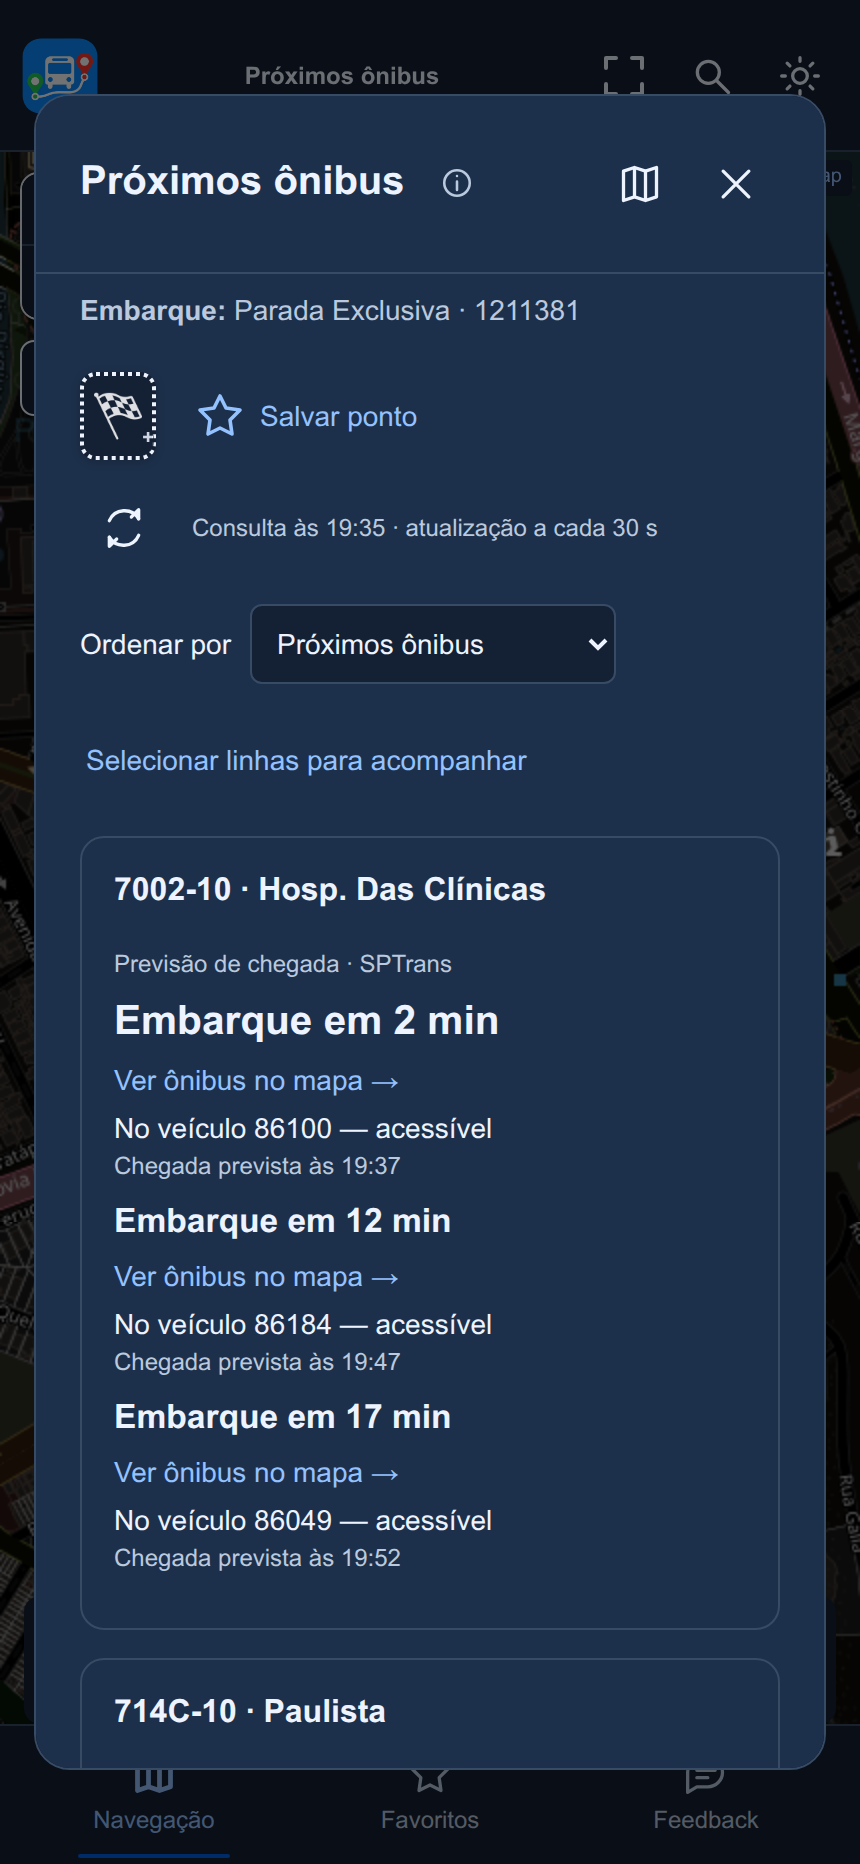
\includegraphics[width=\linewidth]{capturas/2026-10-22/pap-01-embarque.png}
\end{minipage}\hfill
\begin{minipage}[c]{0.60\textwidth}\centering
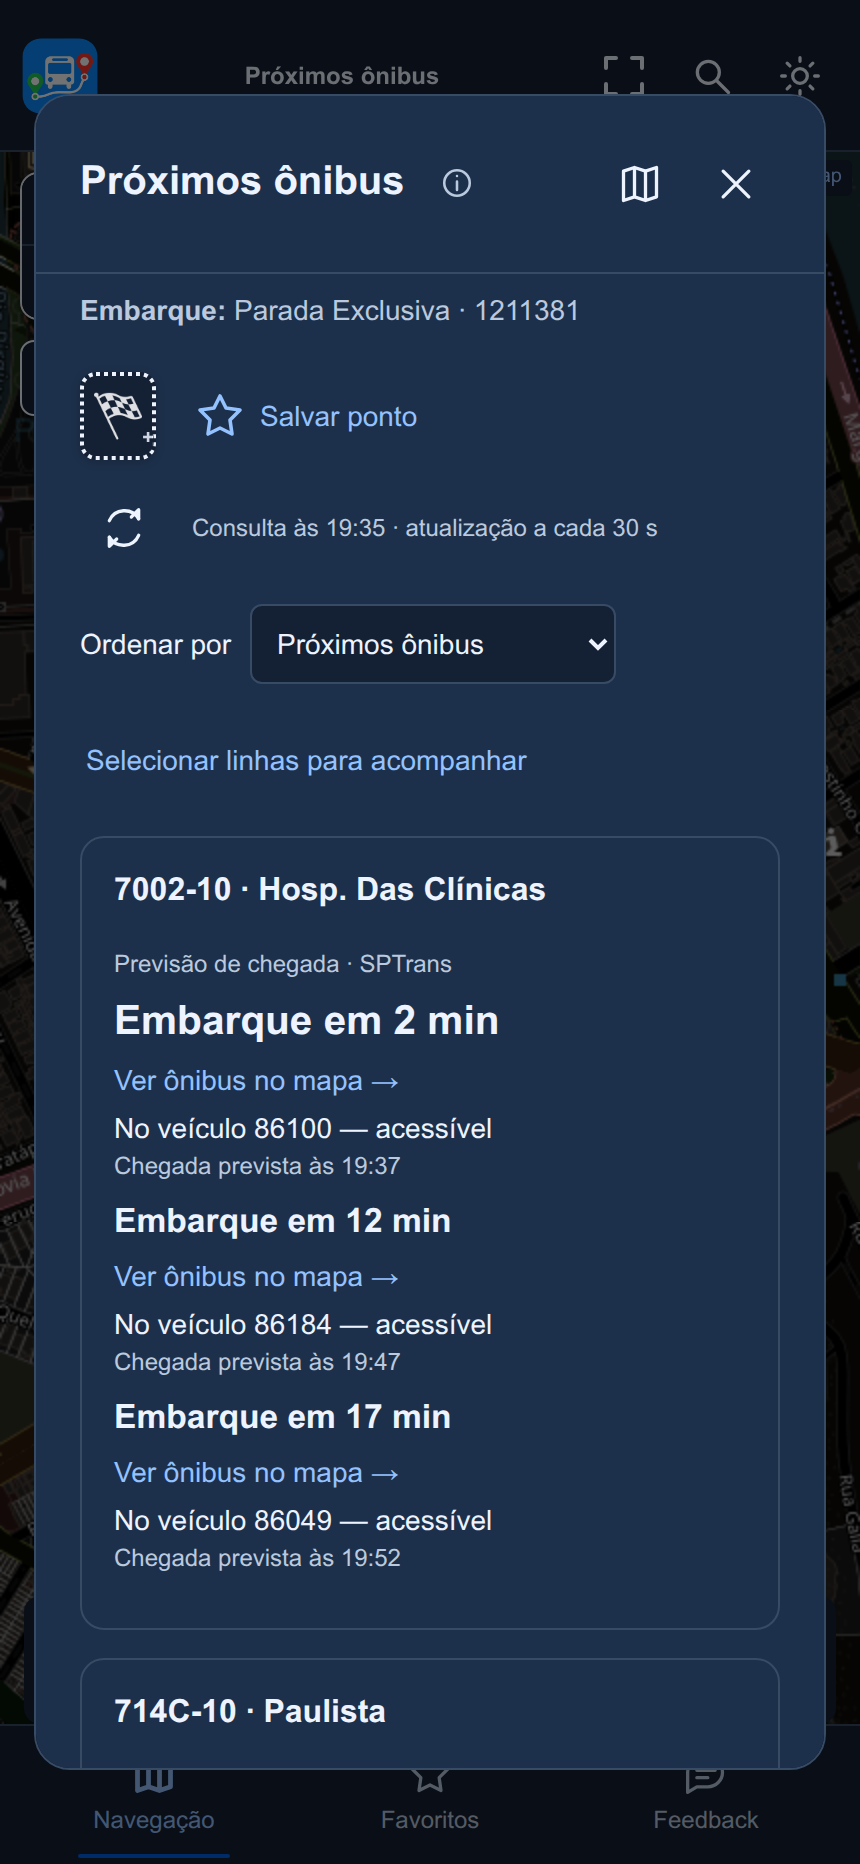
\includegraphics[width=\linewidth,trim=75bp 224bp 70bp 820bp,clip]{capturas/2026-10-22/pap-01-embarque.png}
\small Detalhe ampliado da mesma captura.
\end{minipage}
\caption{Consulta dos próximos ônibus: tela completa e detalhe das previsões.}\label{fig:print-01-embarque}
\fonte{Captura da aplicação em emulação móvel, 22 out. 2026.}
\end{figure}
A consulta foi aberta pelo endereço local da Parada Exclusiva (1211381), no Butantã. O painel distingue previsões operacionais e informações programadas. Os horários são os retornados na captura e não constituem promessa de chegada.
\clearpage

\begin{figure}[H]\centering
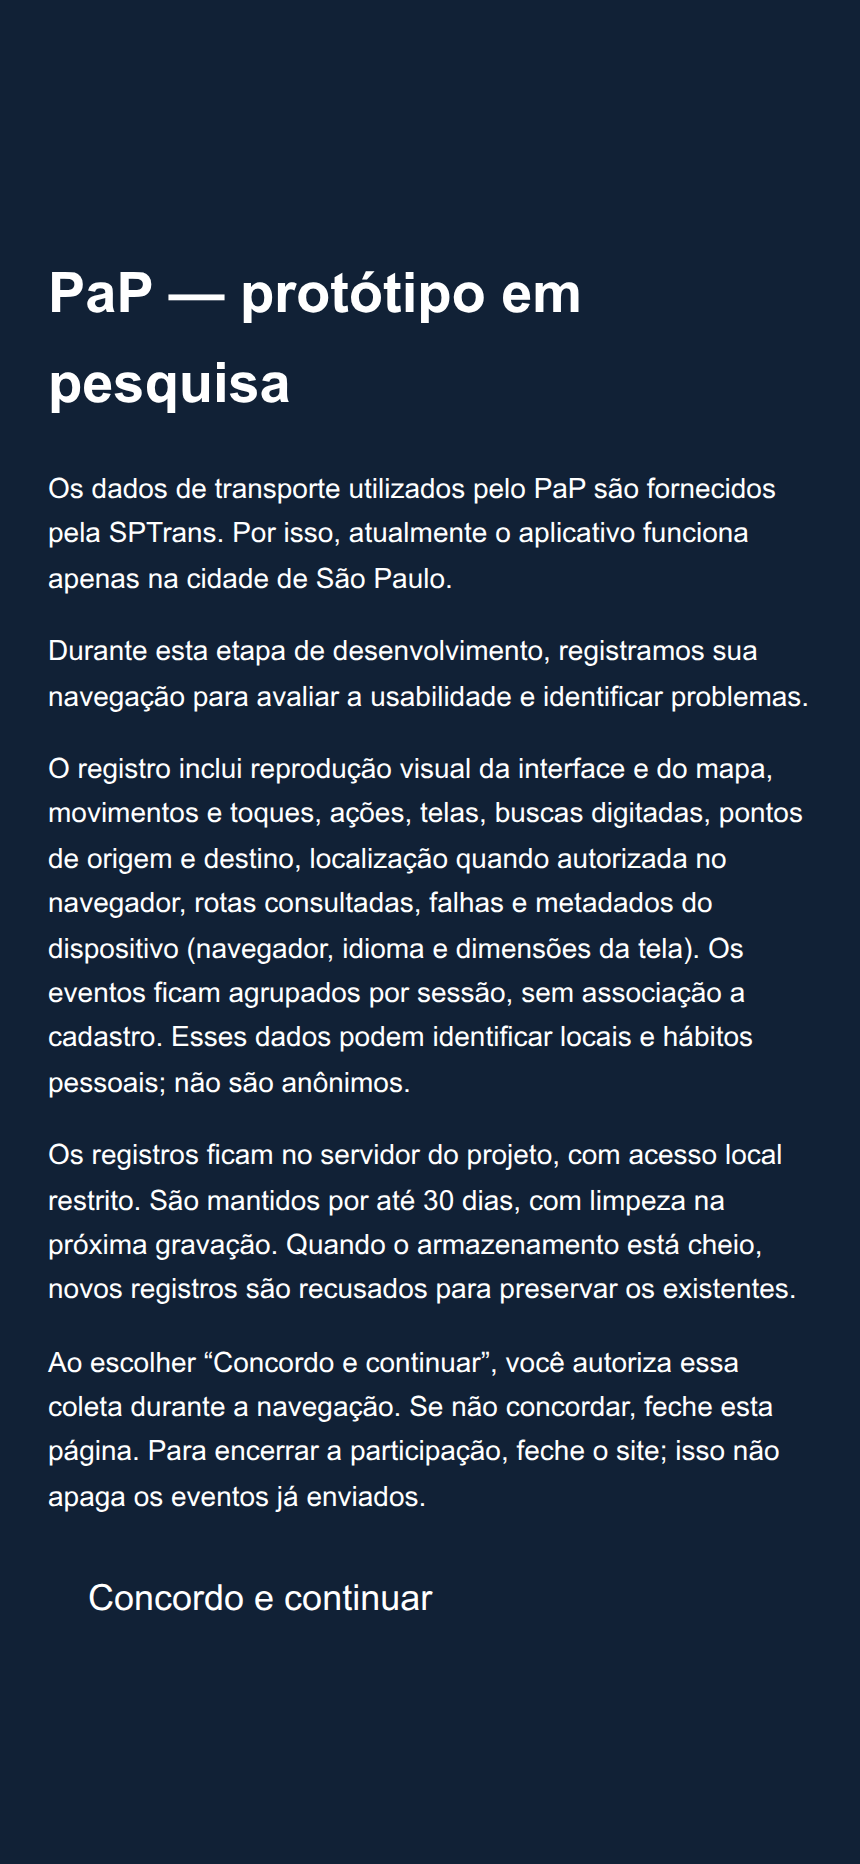
\includegraphics[width=0.80\textwidth,height=0.69\textheight,keepaspectratio,trim=30bp 200bp 30bp 250bp,clip]{capturas/2026-10-22/pap-00-aceite.png}
\caption{Aviso inicial sobre cobertura geográfica e coleta de dados de navegação (recorte das margens vazias).}\label{fig:print-02-informacoes}
\fonte{Captura da aplicação em emulação móvel, 22 out. 2026.}
\end{figure}
O aceite informa que os dados de transporte são fornecidos pela SPTrans e que o PaP funciona atualmente apenas na cidade de São Paulo. A tela também explica os registros de pesquisa e solicita a concordância antes de iniciar a navegação. Esta captura substitui a antiga ilustração conceitual de instalação de uma placa; não houve registro de instalação física.
\clearpage

\begin{figure}[H]\centering
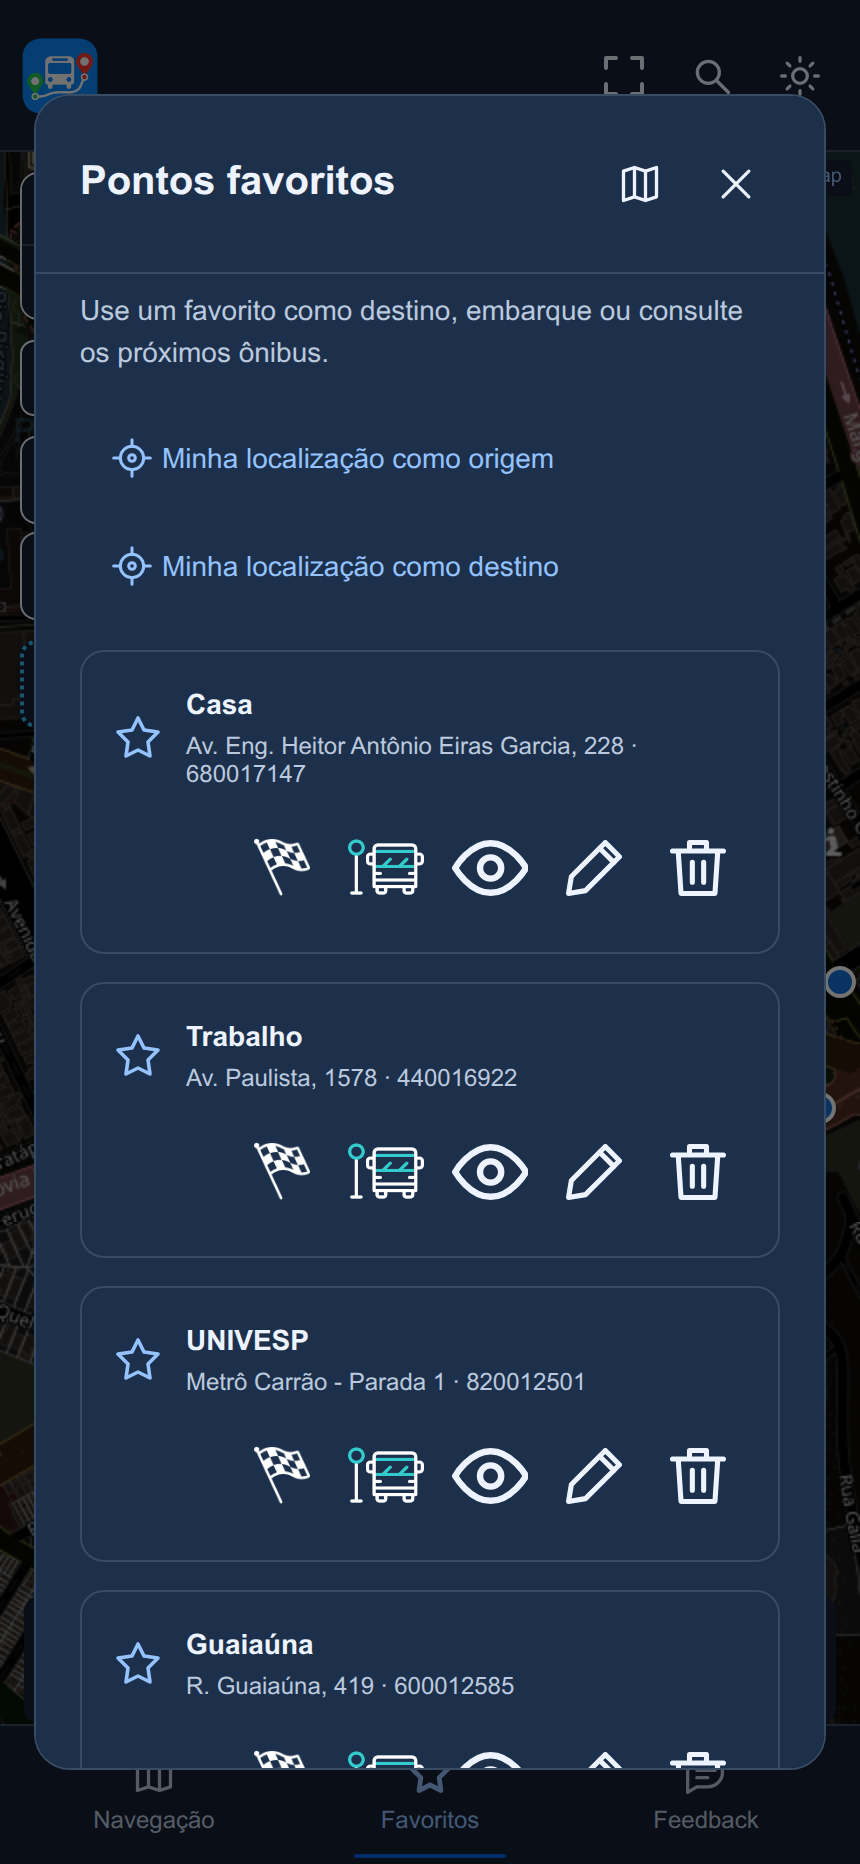
\includegraphics[width=0.80\textwidth,height=0.68\textheight,keepaspectratio]{capturas/2026-10-22/pap-03-destino.png}
\caption{Seleção de destino por pontos favoritos.}\label{fig:print-03-destino}
\fonte{Captura da aplicação em emulação móvel, 22 out. 2026.}
\end{figure}
Os favoritos foram preparados para a documentação com pontos reais e nomes ilustrativos: Casa, Trabalho, UNIVESP e Guaiaúna. Os atalhos permitem escolher destino, embarque ou consulta de próximos ônibus.
\clearpage

\begin{figure}[H]\centering
\begin{minipage}[c]{0.36\textwidth}\centering
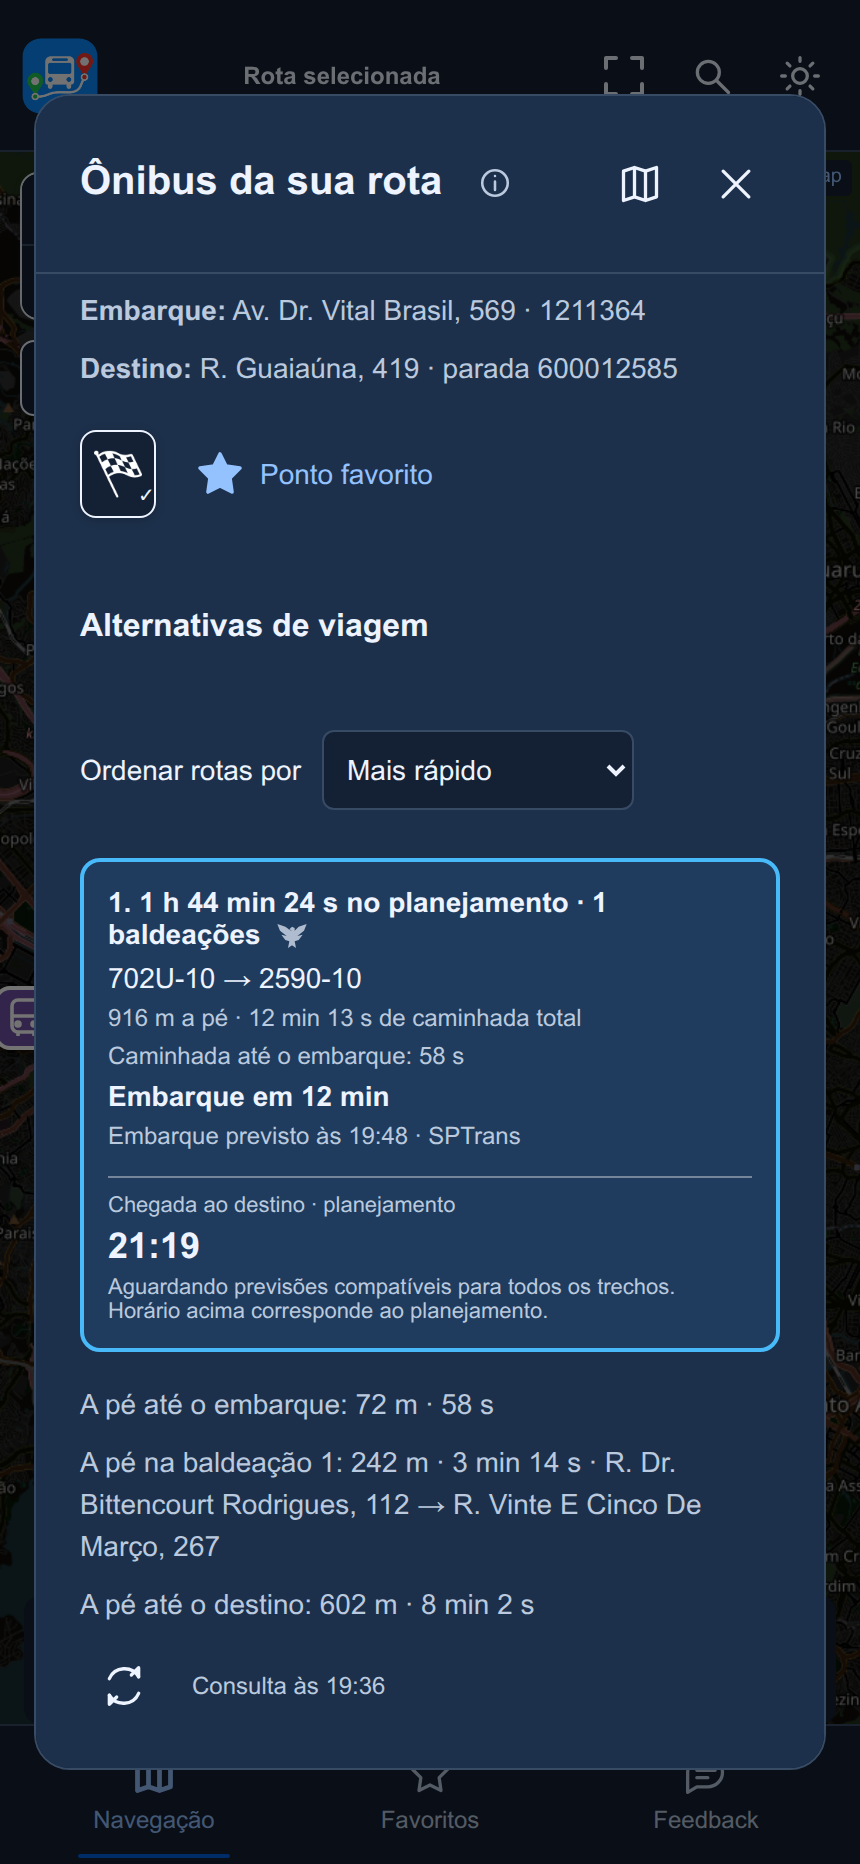
\includegraphics[width=\linewidth]{capturas/2026-10-22/pap-04-alternativas.png}
\end{minipage}\hfill
\begin{minipage}[c]{0.60\textwidth}\centering
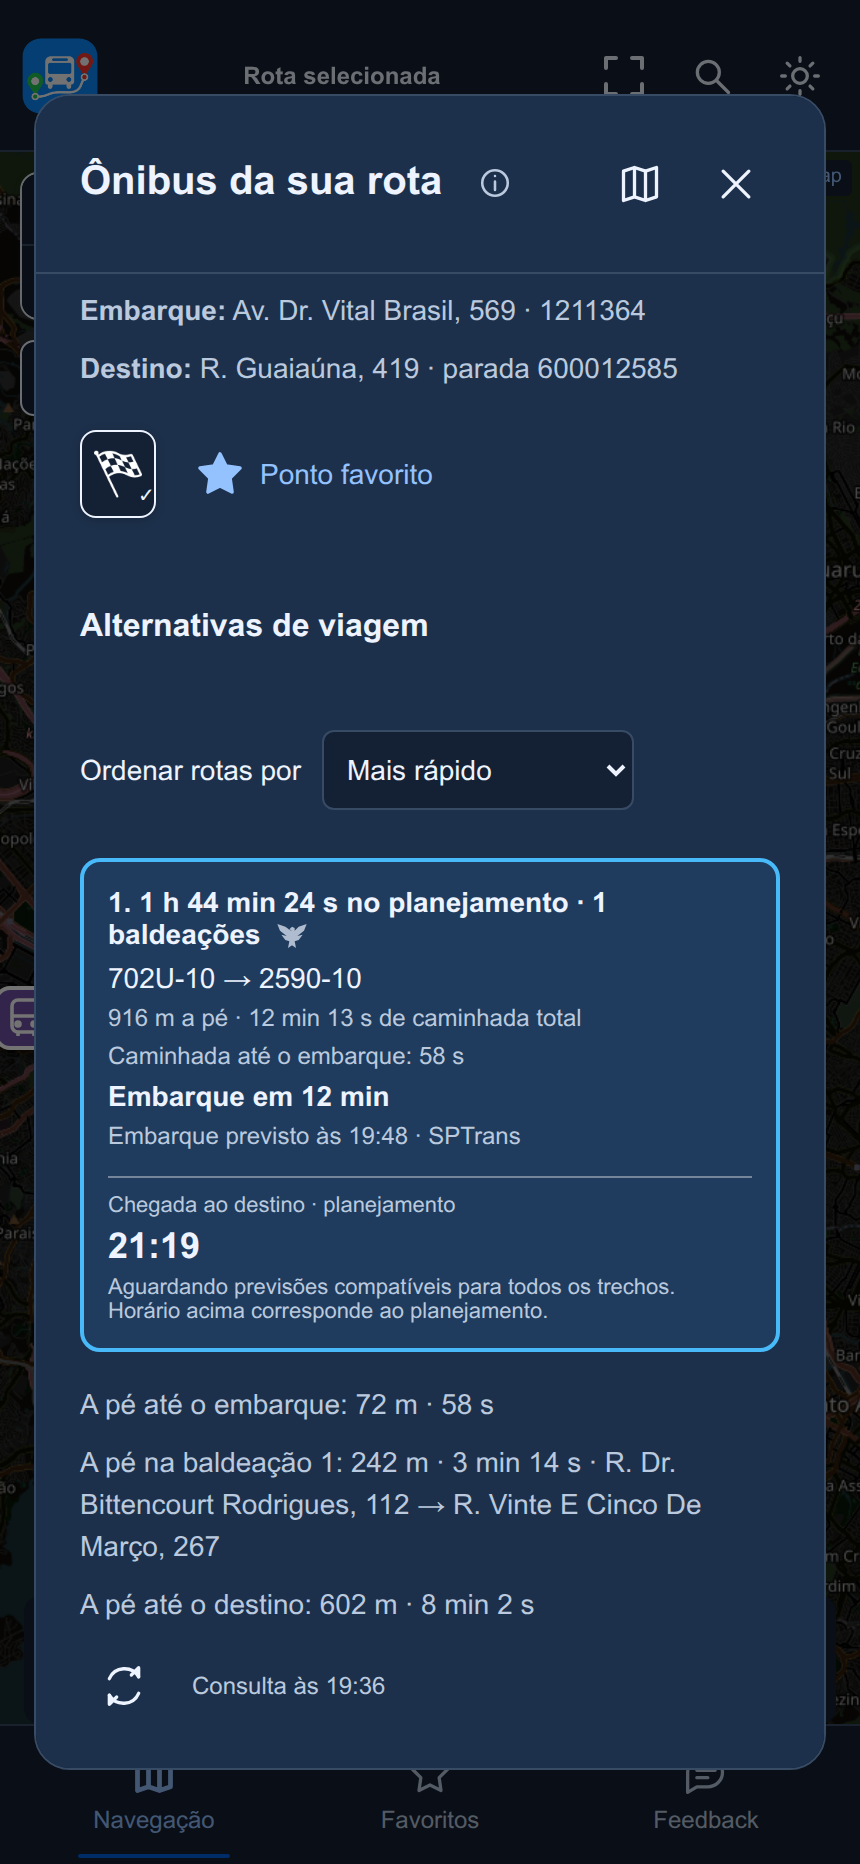
\includegraphics[width=\linewidth,trim=75bp 504bp 70bp 850bp,clip]{capturas/2026-10-22/pap-04-alternativas.png}
\small Detalhe ampliado da mesma captura.
\end{minipage}
\caption{Alternativas de viagem: tela completa e detalhe da alternativa selecionada.}\label{fig:print-04-alternativas}
\fonte{Captura da aplicação em emulação móvel, 22 out. 2026.}
\end{figure}
As capturas integram a mesma sequência registrada no roteiro de captura: acesso à Parada Exclusiva (1211381), retorno ao mapa e seleção de Guaiaúna como destino favorito. O painel de alternativas mostra o embarque do primeiro trecho da rota selecionada, na Av. Dr. Vital Brasil, 569 (1211364), e o destino na Rua Guaiaúna, 419 (600012585). A caminhada de acesso exibida é de 72 m, estimada em 58 s; portanto, o embarque da alternativa difere do ponto usado para iniciar a consulta. O painel apresenta as alternativas calculadas no instante da consulta, com caminhada, baldeações e informações de embarque. Os resultados variam com o horário e com os dados disponíveis.
\clearpage

\begin{figure}[H]\centering
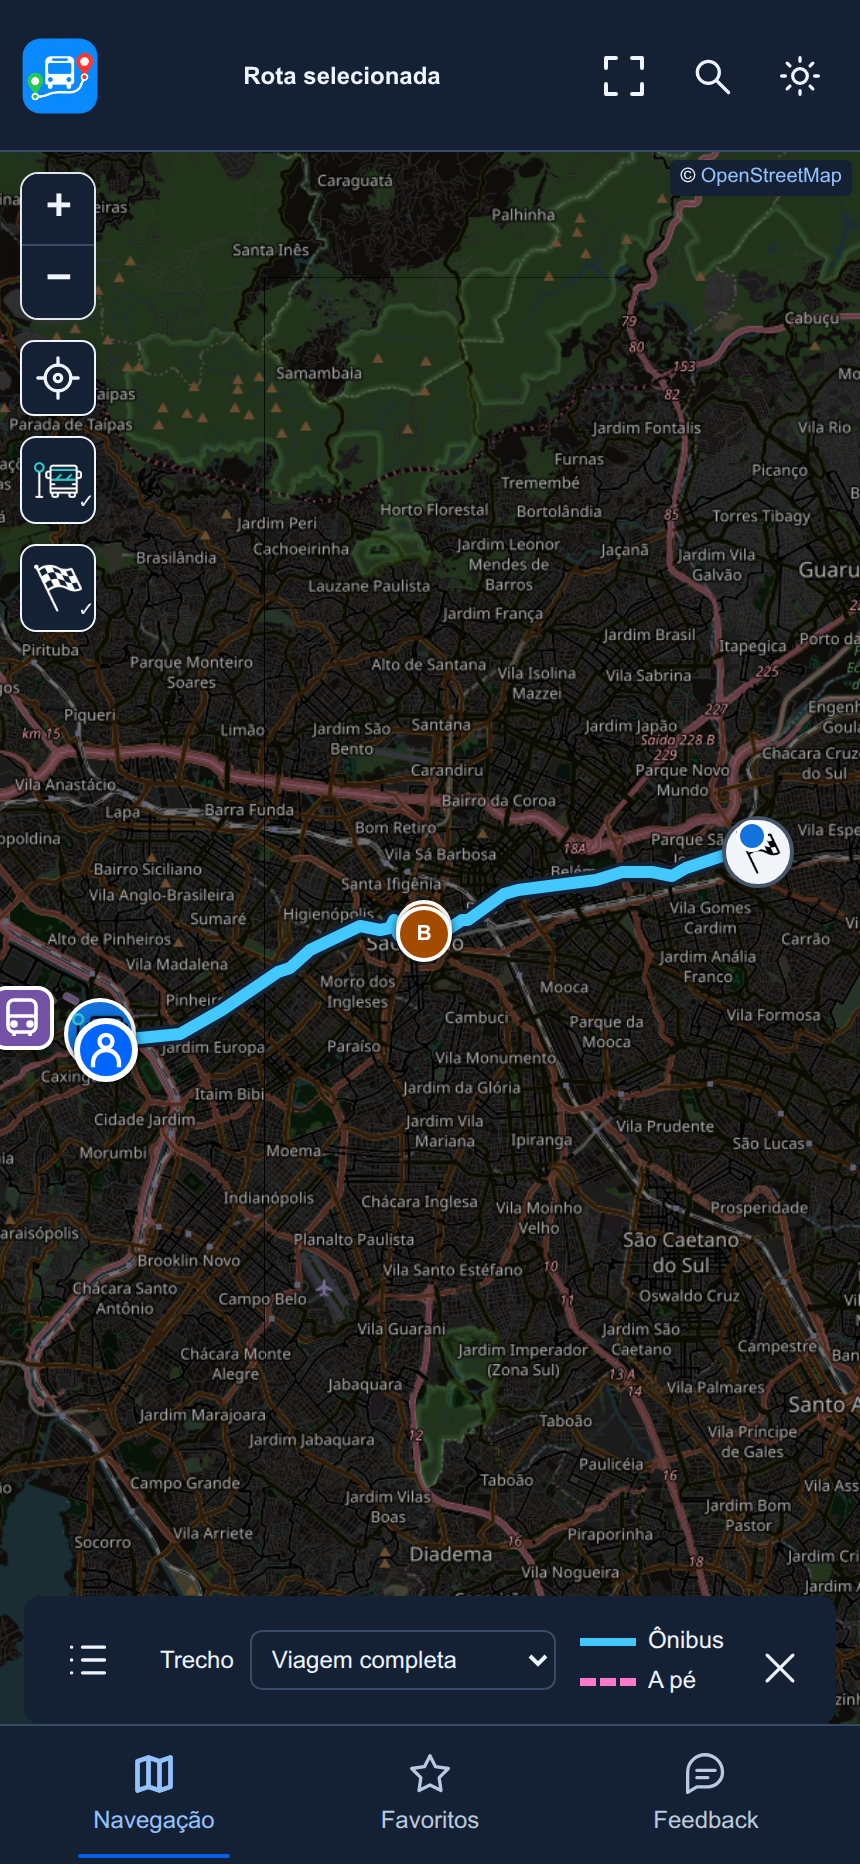
\includegraphics[width=0.80\textwidth,height=0.68\textheight,keepaspectratio]{capturas/2026-10-22/pap-05-viagem-completa.png}
\caption{Viagem completa, com embarque, baldeação e destino.}\label{fig:print-05-viagem-completa}
\fonte{Captura da aplicação em emulação móvel, 22 out. 2026.}
\end{figure}
A rota selecionada é representada no mapa. A legenda distingue trechos de ônibus e caminhada; o controle inferior permite retornar à lista ou selecionar um trecho quando houver baldeação.
\clearpage

\begin{figure}[H]\centering
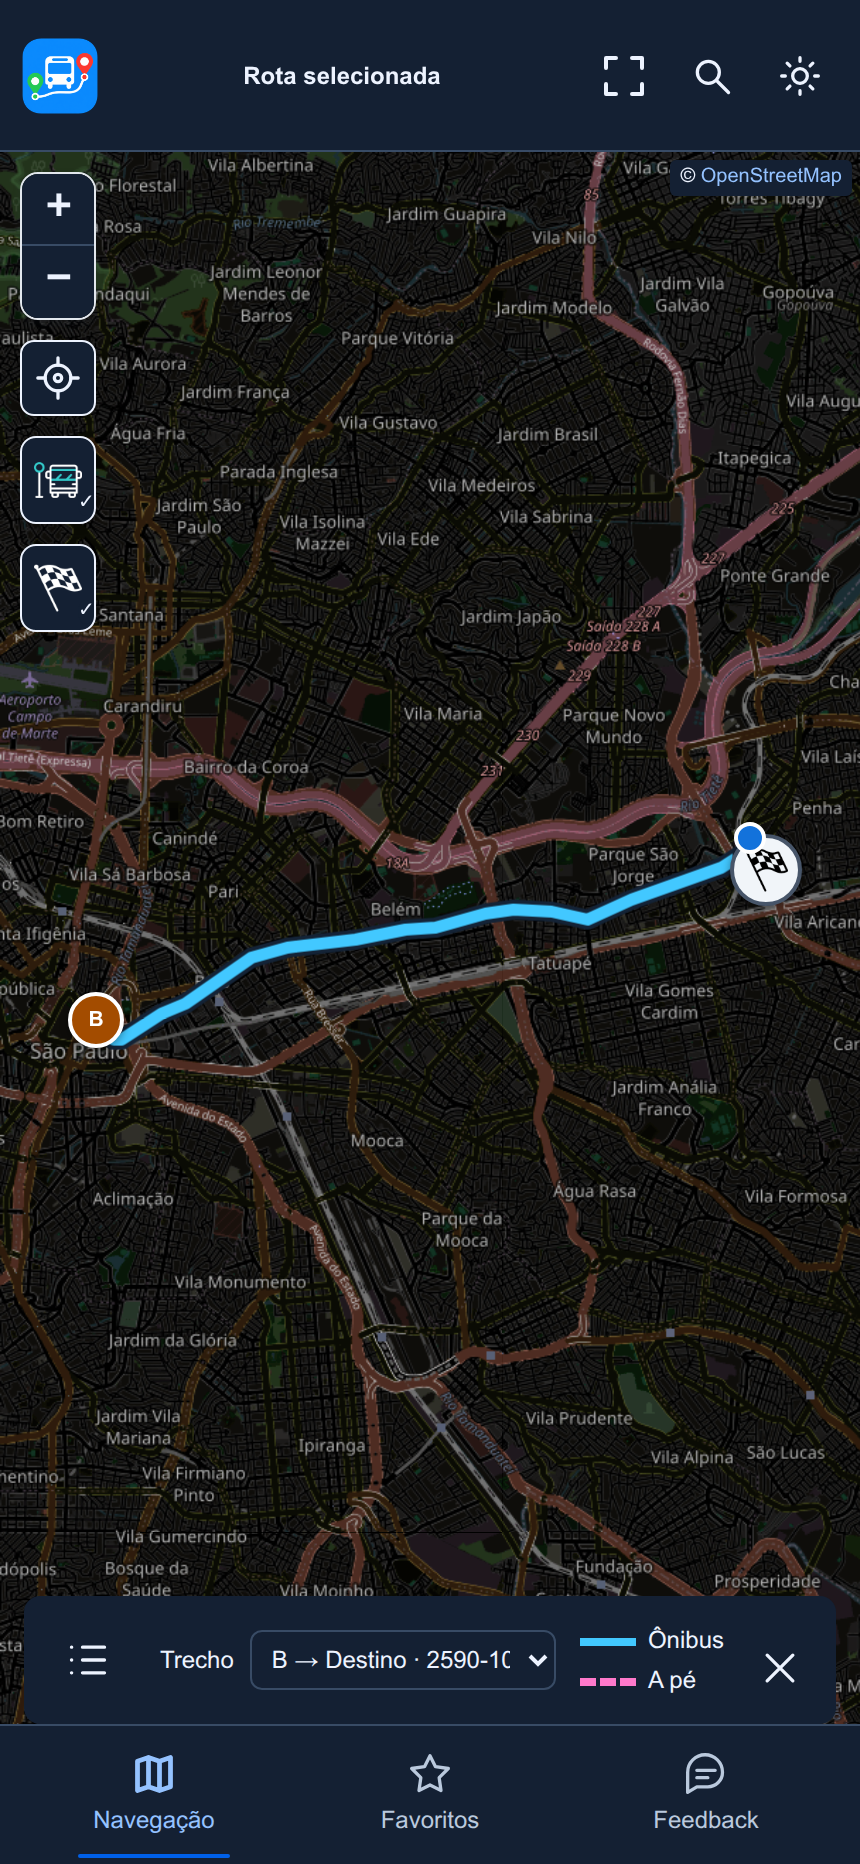
\includegraphics[width=0.80\textwidth,height=0.68\textheight,keepaspectratio]{capturas/2026-10-22/pap-06-ultimo-trecho.png}
\caption{Visualização do último trecho da viagem selecionada.}\label{fig:print-06-ultimo-trecho}
\fonte{Captura da aplicação em emulação móvel, 22 out. 2026.}
\end{figure}
O seletor de trechos permite examinar a parte final do percurso sem perder a referência da viagem escolhida.
\clearpage

\begin{figure}[H]\centering
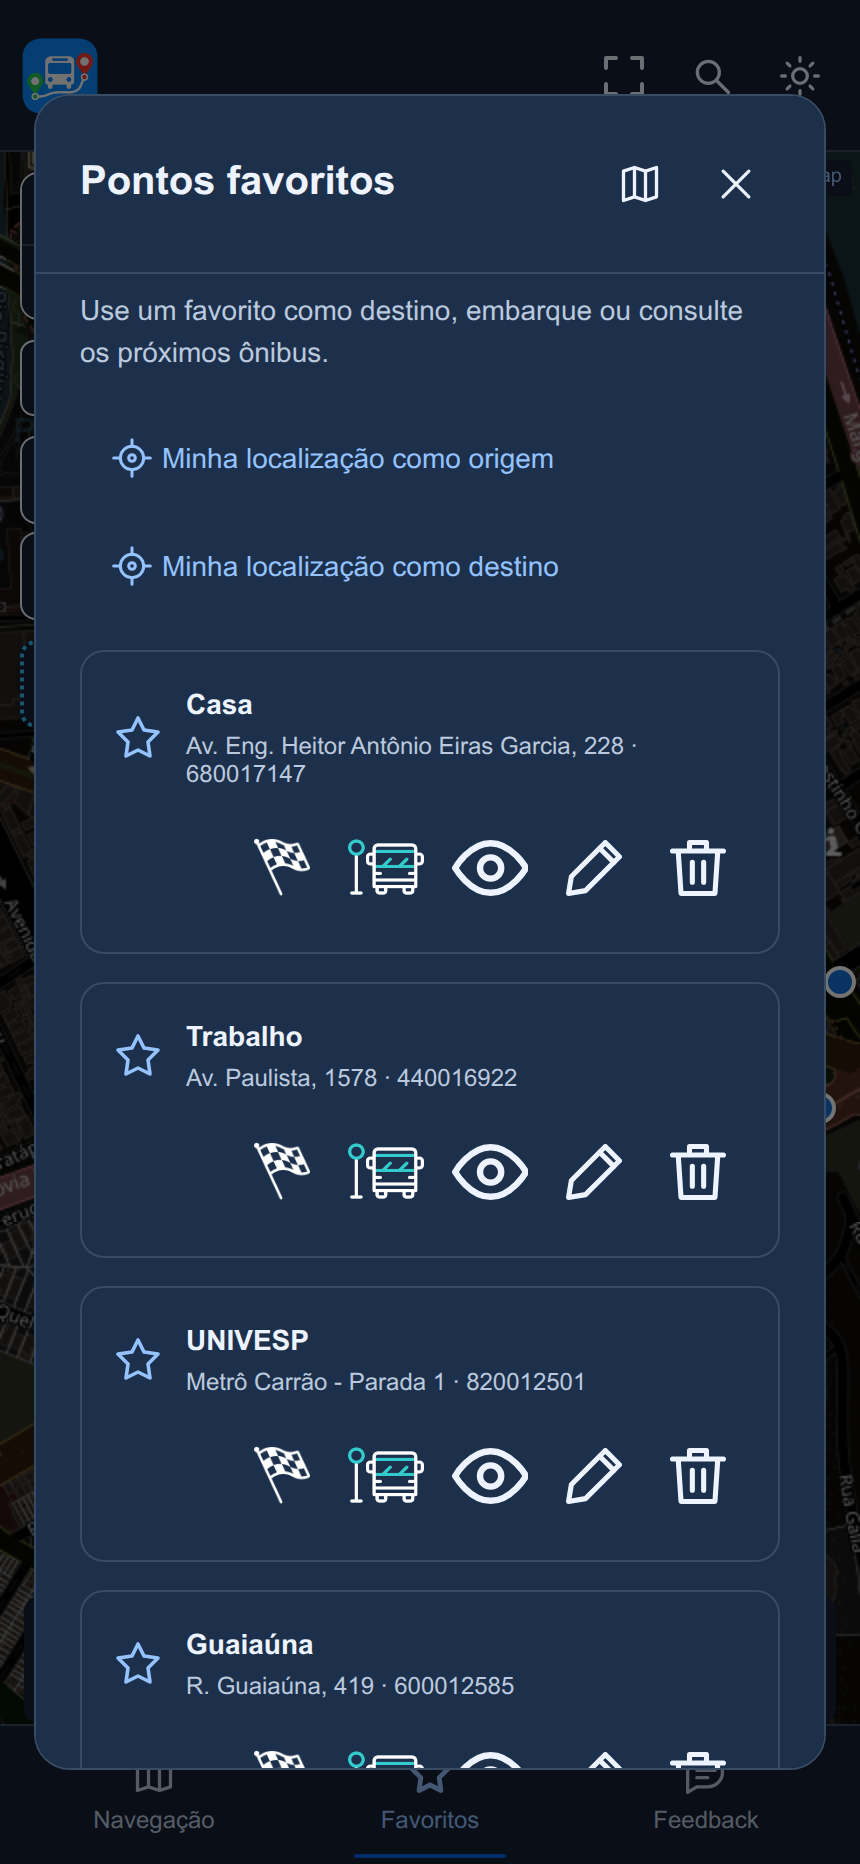
\includegraphics[width=0.80\textwidth,height=0.68\textheight,keepaspectratio]{capturas/2026-10-22/pap-07-favoritos.png}
\caption{Favoritos nomeados e ações disponíveis para cada ponto.}\label{fig:print-07-favoritos}
\fonte{Captura da aplicação em emulação móvel, 22 out. 2026.}
\end{figure}
Os ícones oferecem ações de destino, embarque, consulta, renomeação e remoção. Os nomes salvos para esta captura são exemplos de organização pessoal.
\clearpage

\begin{figure}[H]\centering
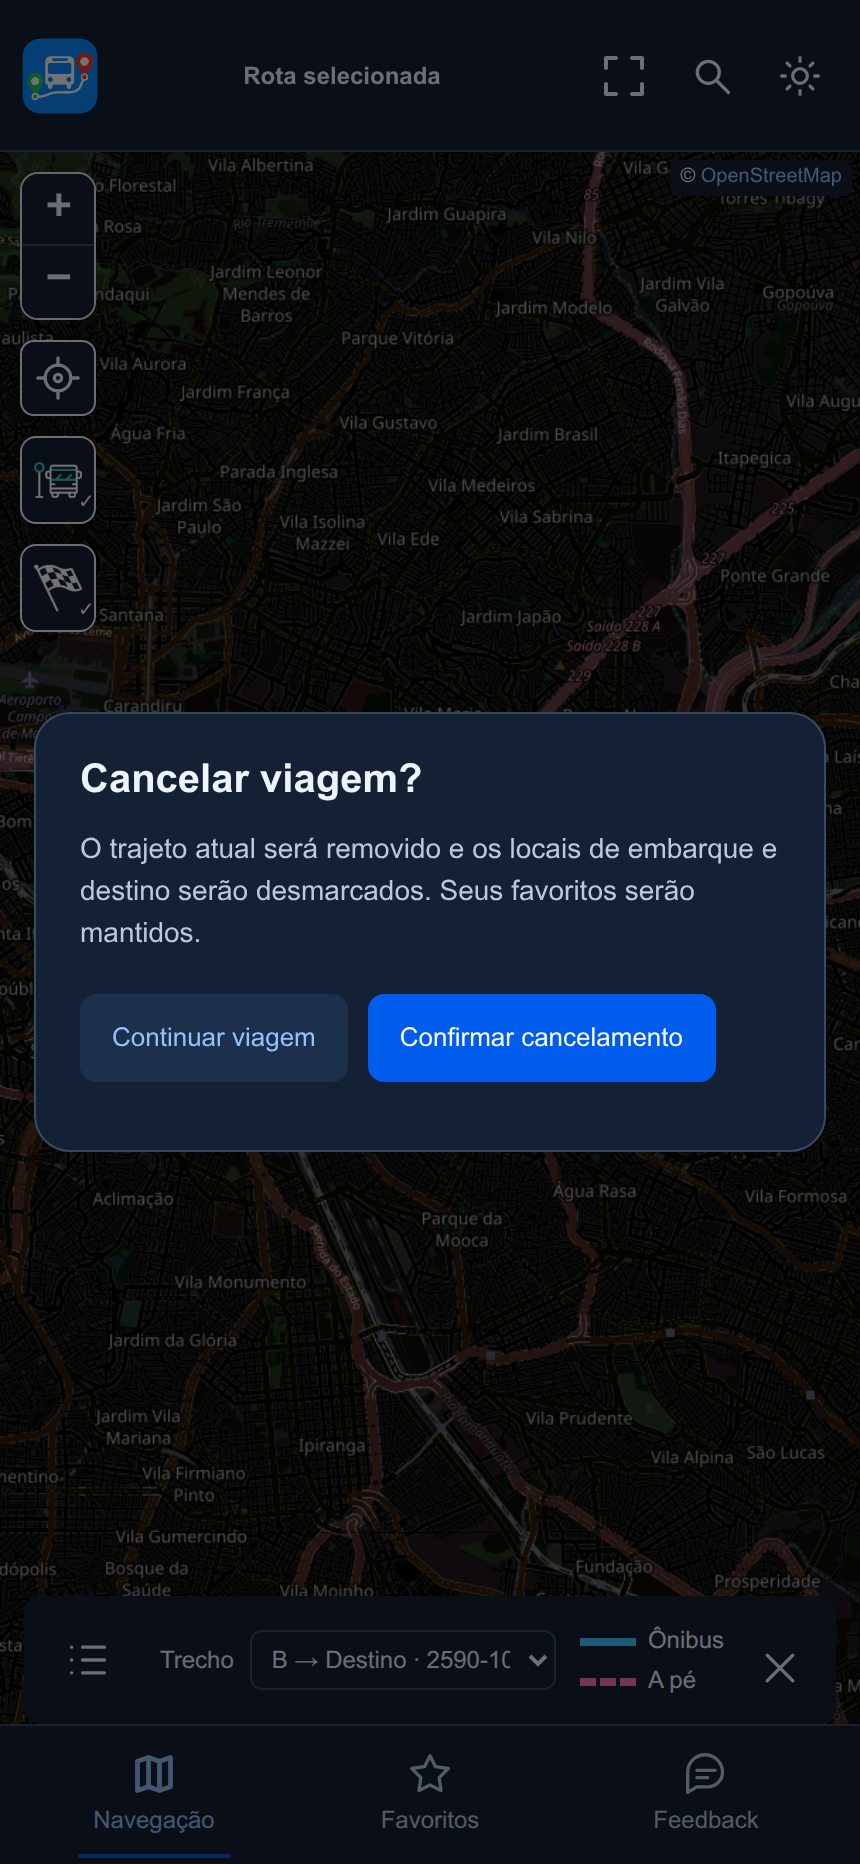
\includegraphics[width=0.80\textwidth,height=0.68\textheight,keepaspectratio]{capturas/2026-10-22/pap-08-confirmacao.png}
\caption{Confirmação antes de cancelar a viagem.}\label{fig:print-08-confirmacao}
\fonte{Captura da aplicação em emulação móvel, 22 out. 2026.}
\end{figure}
O diálogo explica que o trajeto e os locais de embarque e destino serão desmarcados, preservando os favoritos. O passageiro pode continuar a viagem ou confirmar o cancelamento.
\clearpage

\begin{figure}[H]\centering
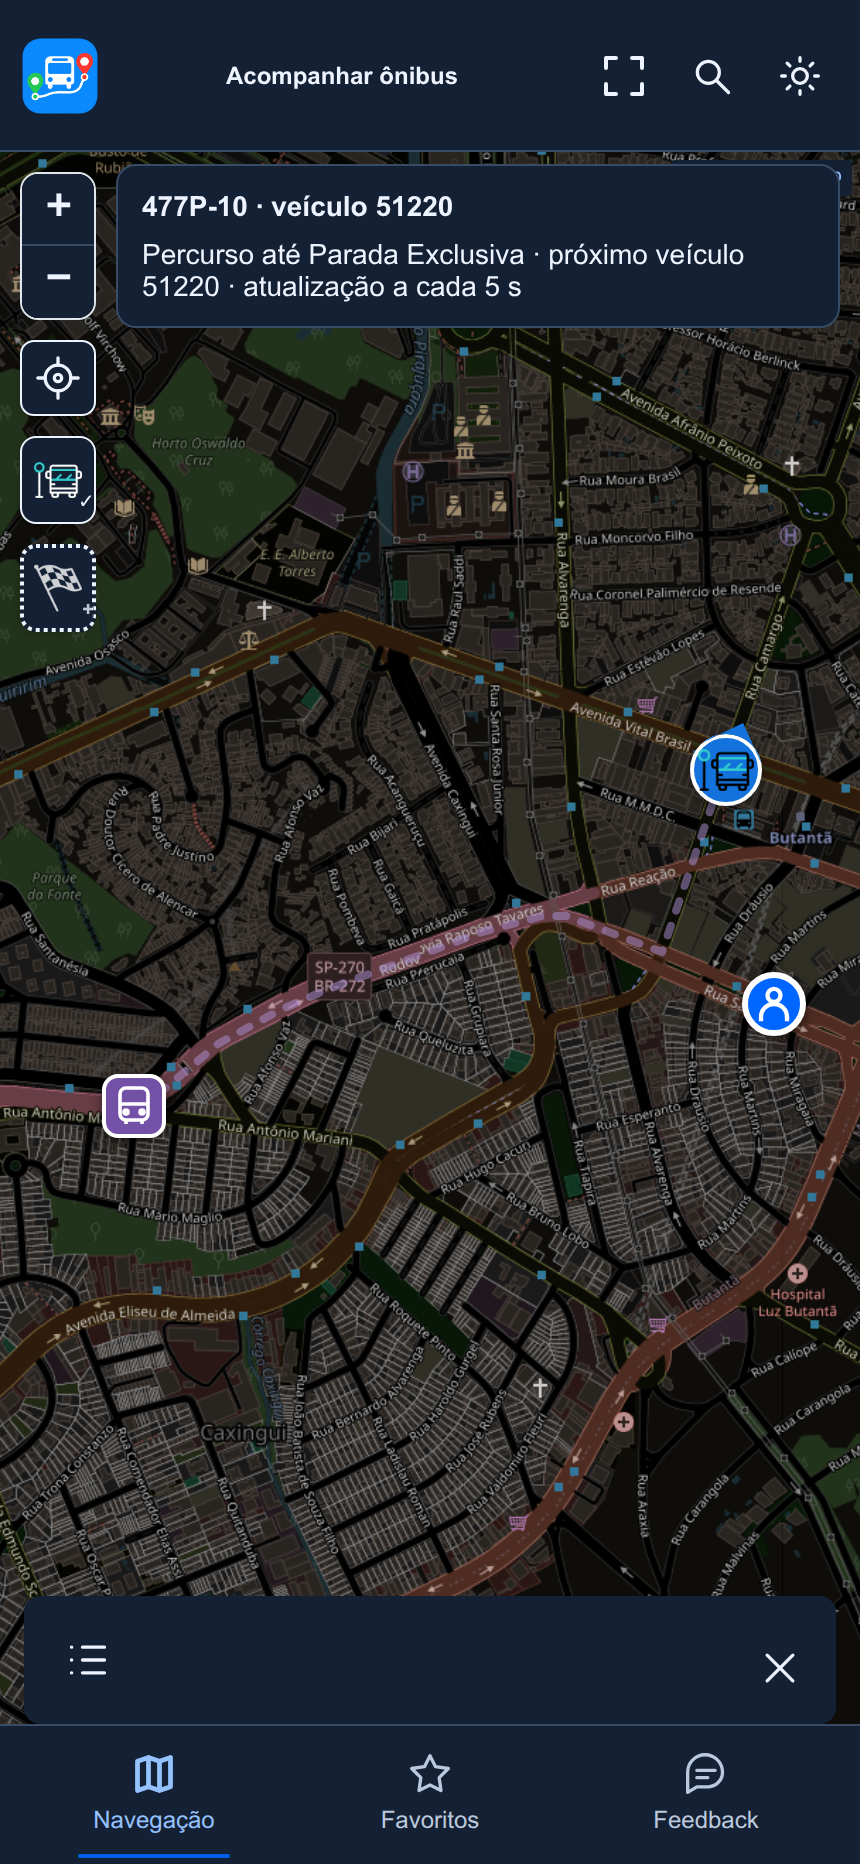
\includegraphics[width=0.80\textwidth,height=0.68\textheight,keepaspectratio]{capturas/2026-10-22/pap-13-onibus-tempo-real.png}
\caption{Acompanhamento de veículo consultado na API Olho Vivo.}\label{fig:print-onibus-tempo-real}
\fonte{Captura da aplicação em emulação móvel, 22 out. 2026.}
\end{figure}
A tela foi aberta pela ação de visualizar um veículo na consulta dos próximos ônibus. O marcador utiliza a posição disponível no serviço externo no momento da captura. Uma imagem estática não comprova atualização periódica nem precisão operacional.
\clearpage
\begin{figure}[H]\centering
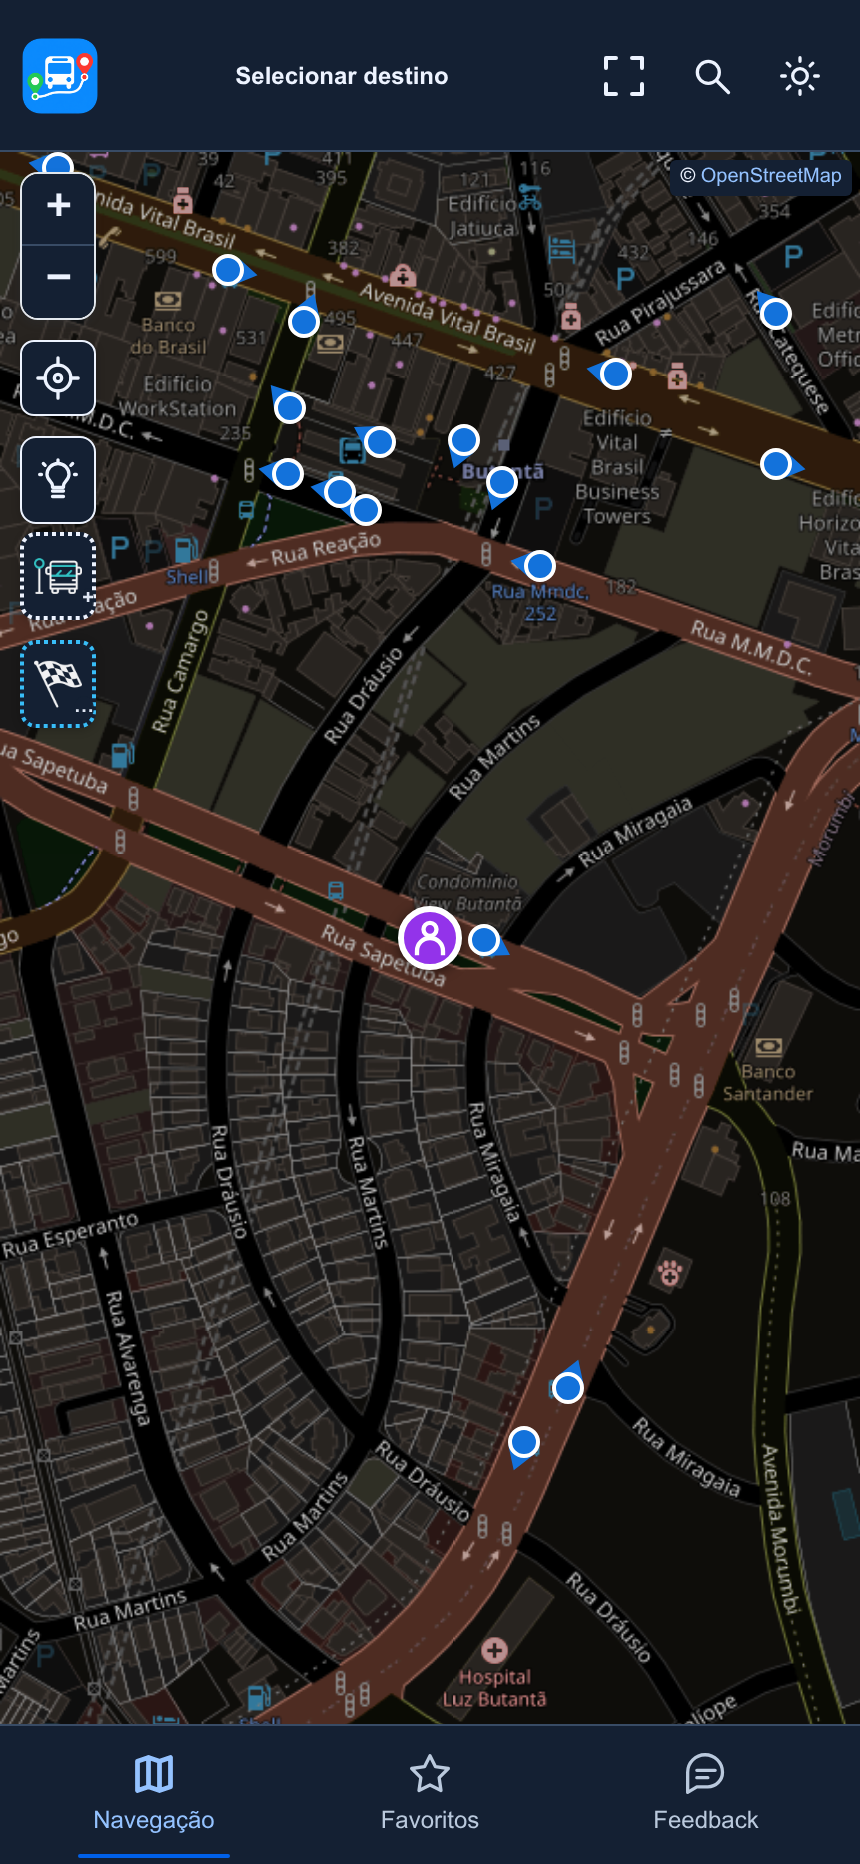
\includegraphics[width=0.43\textwidth,height=0.60\textheight,keepaspectratio]{capturas/2026-10-22/pap-09-localizacao.png}\hfill
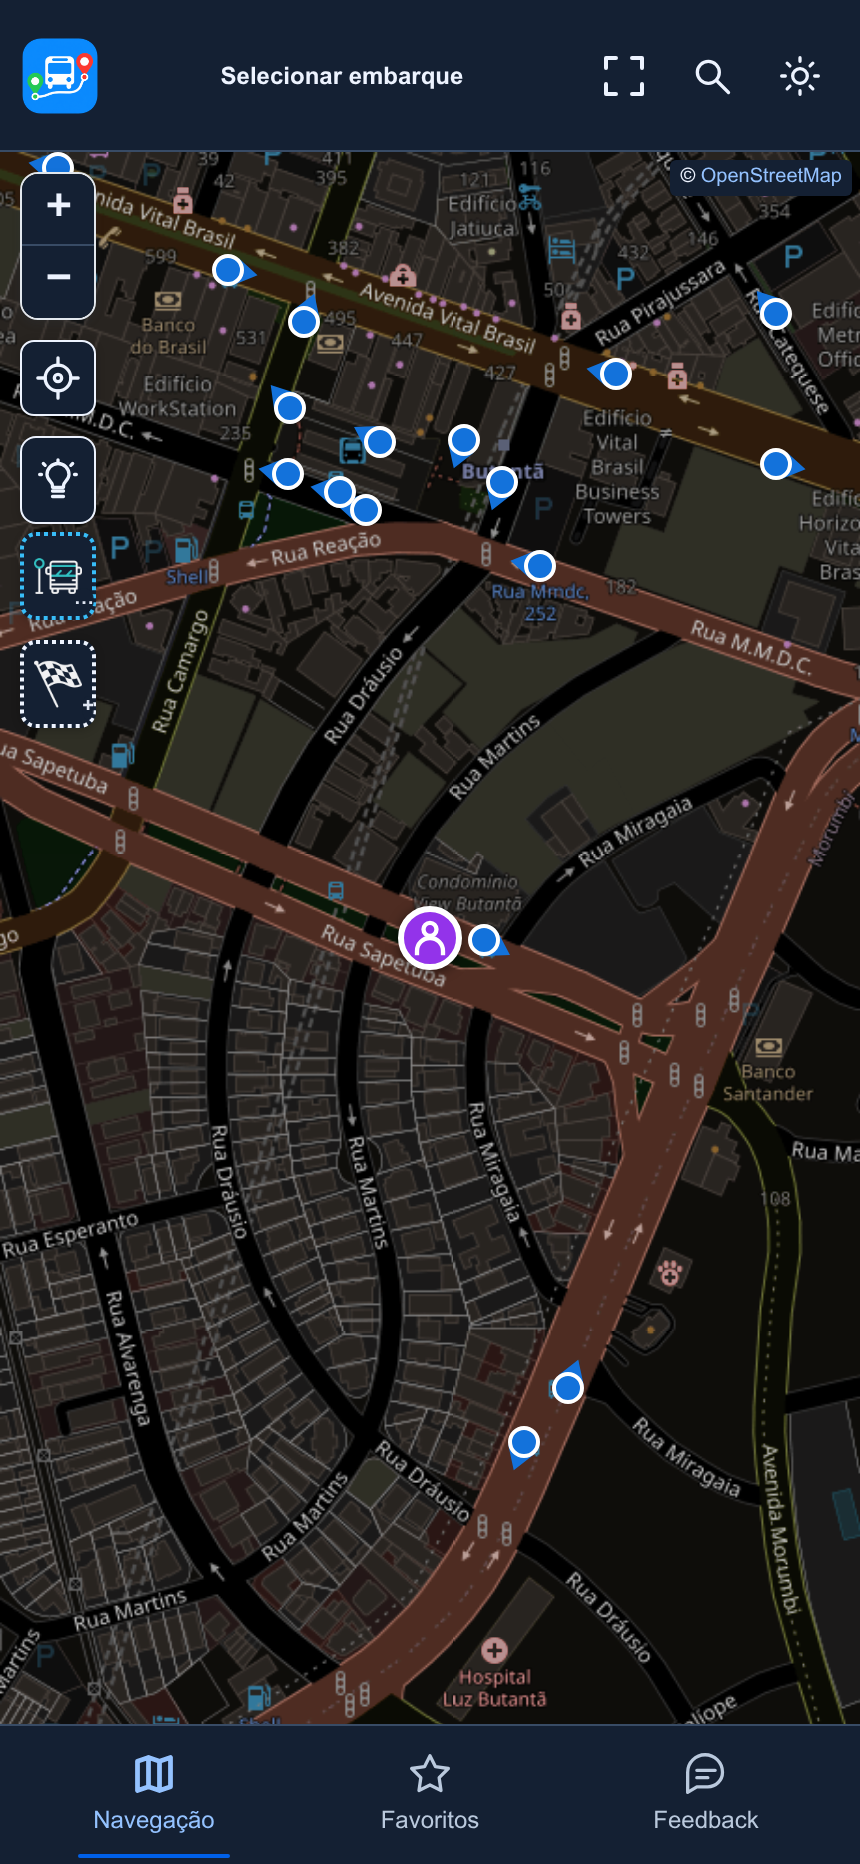
\includegraphics[width=0.43\textwidth,height=0.60\textheight,keepaspectratio]{capturas/2026-10-22/pap-10-alterar-embarque.png}
\caption{Localização simulada como origem (à esquerda) e seleção manual do embarque (à direita).}\label{fig:print-localizacao}
\fonte{Capturas da aplicação em emulação móvel, 22 out. 2026.}
\end{figure}
O marcador roxo indica a localização simulada. O controle lateral permite escolher uma parada de embarque no mapa. O cabeçalho utiliza a expressão Selecionar embarque; a navegação inferior inclui o acesso ao feedback.
\clearpage

\begin{figure}[H]\centering
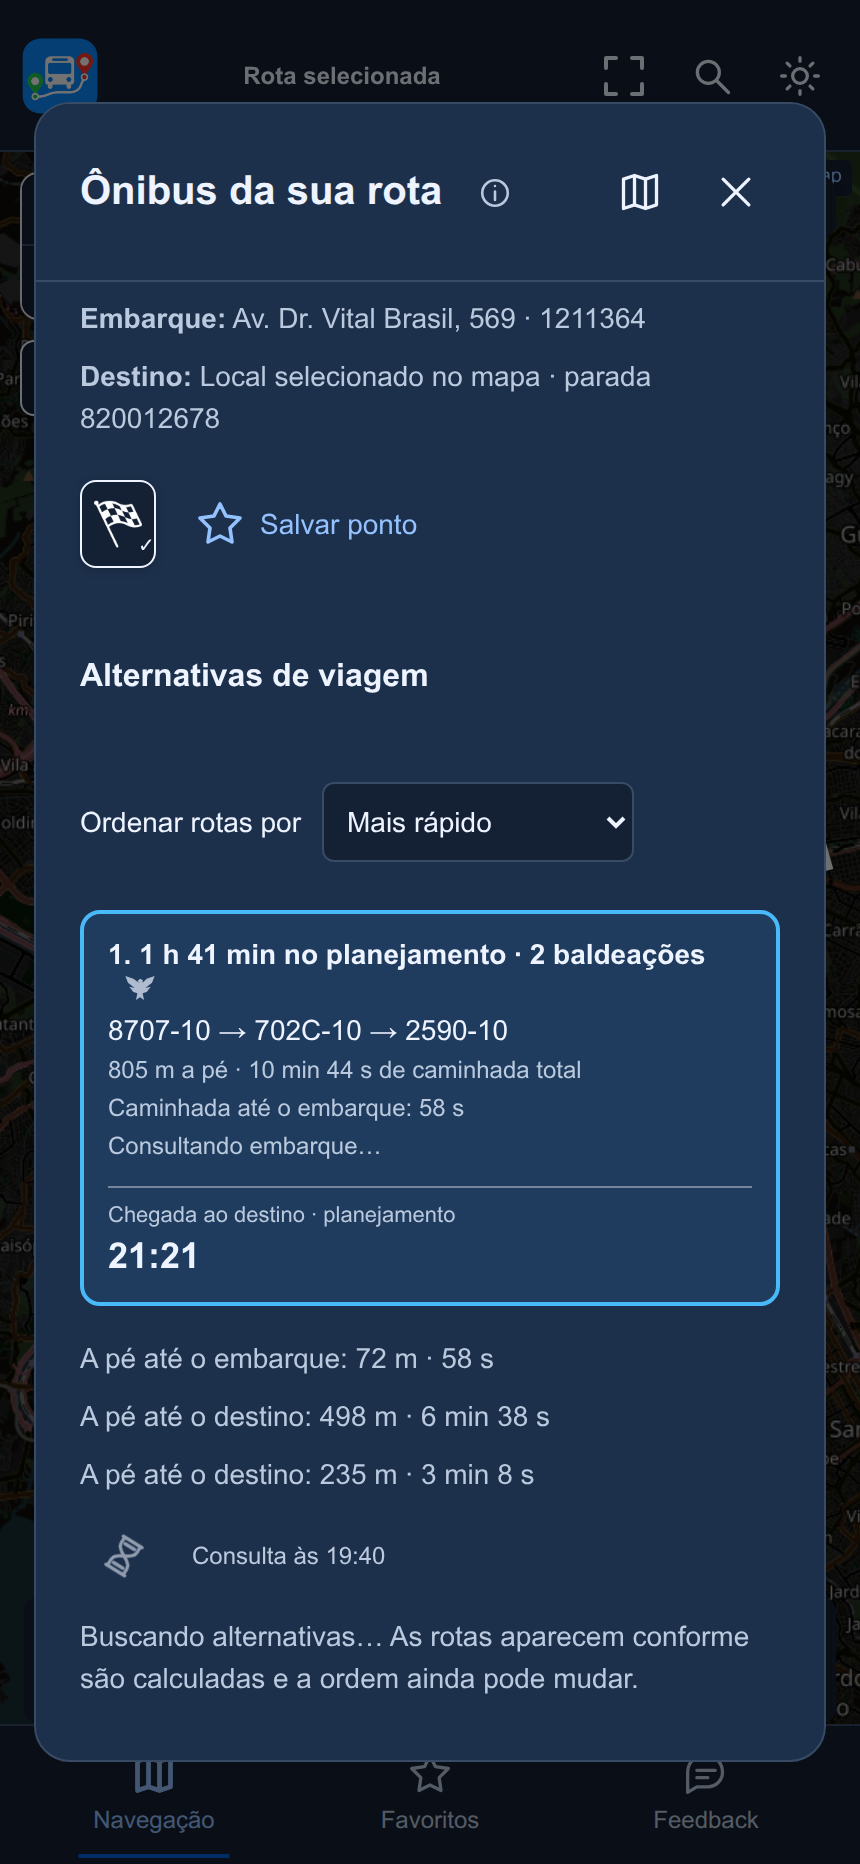
\includegraphics[width=0.80\textwidth,height=0.68\textheight,keepaspectratio]{capturas/2026-10-22/pap-12-destino-livre.png}
\caption{Destino definido por toque prolongado no mapa.}\label{fig:print-destino-livre}
\fonte{Captura da aplicação em emulação móvel, 22 out. 2026.}
\end{figure}
A busca por coordenadas centralizou a região desejada e o toque prolongado definiu um local de destino. O painel apresenta alternativas progressivamente e, no instante capturado, ainda consulta informações de embarque. A imagem não representa o encerramento de todas as consultas.
\clearpage

\begin{figure}[H]\centering
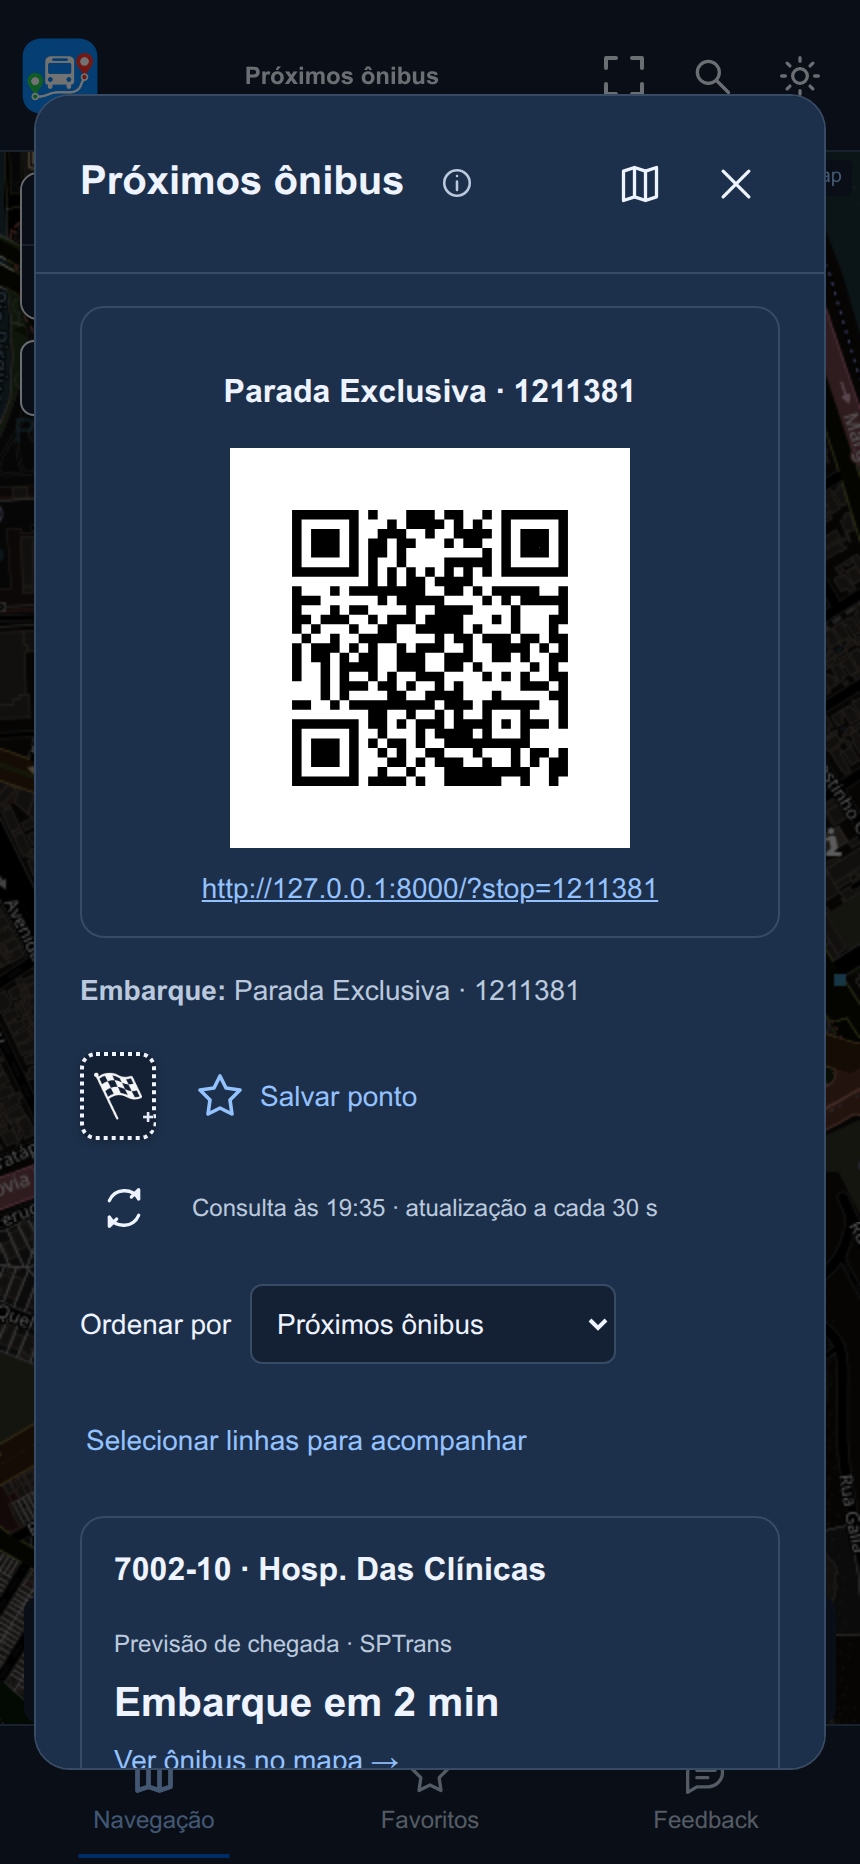
\includegraphics[width=0.80\textwidth,height=0.68\textheight,keepaspectratio]{capturas/2026-10-22/pap-14-qr-atual.png}
\caption{Informações da parada e QR Code de acesso à consulta.}\label{fig:print-qr-atual}
\fonte{Captura da aplicação em emulação móvel, 22 out. 2026.}
\end{figure}
A tela utiliza o identificador 1211381 e o endereço local de desenvolvimento. A captura documenta a geração do QR Code; não demonstra leitura física pela câmera. Para uso externo, é necessário um endereço HTTPS acessível aos passageiros.
\clearpage

A apresentação conserva os registros históricos do cenário de Mauá e acrescenta a evolução técnica de São Paulo, examinada na revisão \texttt{4992027}, de 7 de outubro de 2026. Essa extensão utiliza o cadastro GTFS da SPTrans e consulta o Olho Vivo quando o serviço e a identificação de linha e parada permitem. Horários programados representam a programação do serviço e não previsões operacionais em tempo real. A extensão não altera a comunidade originalmente delimitada nem comprova disponibilidade de dados equivalentes em Mauá.

Na interface dessa extensão, a localização conhecida identifica automaticamente a origem e permite selecionar apenas o destino; o QR Code mantém a entrada por parada. O mapa inicia centrado no passageiro, com raio mínimo de 250 m no menor eixo, e permite recentrar pela ação de localização. Coordenadas simuladas configuráveis do passageiro substituem seu GPS para reprodução de cenários; quando ausentes, utiliza-se a localização autorizada pelo navegador. Além disso, os favoritos permitem reutilizar destinos e a seleção de uma alternativa abre seu percurso no mapa. O cálculo fornece resultados progressivos e preserva a seleção e o enquadramento do mapa durante atualizações. Essas escolhas procuram reduzir operações repetidas e tornar o estado da consulta perceptível, em consonância com os critérios de IHC discutidos. Sua implementação é um resultado técnico; a redução efetiva do esforço do passageiro permanece por medir.


O toque prolongado por aproximadamente 0,65 segundo permite selecionar coordenadas fora das paradas, respeitando a tarefa ativa: origem ao alterar o embarque ou destino ao escolher a chegada. Arrasto e gestos com dois dedos cancelam a seleção. O planejamento inclui as caminhadas entre essas coordenadas e as paradas utilizadas. Alterar o embarque conserva o destino e reenquadra o mapa na localização do passageiro ou, na sua ausência, no embarque anterior. Confirmar o cancelamento remove o trajeto, mantém o embarque e retorna à seleção de destino com foco no destino anterior.

A tela de rotas utiliza uma ampulheta animada durante o cálculo e disponibiliza o recálculo manual ao concluir. Reiniciar a busca ignora o cache de resultados e executa novamente o planejamento. A consulta de rotas não é reiniciada automaticamente a cada 30 segundos nem a cada atualização do GPS; a atualização periódica permanece na consulta de próximos ônibus. No mapa, o seletor Trecho alterna a viagem completa e suas etapas, com legenda de ônibus e caminhada em coluna. A consulta de próximos ônibus apresenta a frequência como intervalo entre veículos e a faixa em que ele vigora, unindo faixas consecutivas de mesma frequência. Essa apresentação evita confundir frequência com contagem regressiva para a chegada. A identidade visual utiliza ícone próprio, mantendo a identificação das fontes de dados na documentação e nas informações da aplicação.

Nesta etapa, a proposta de iniciar a consulta pelo ponto de ônibus foi materializada em um protótipo que permite demonstrar o percurso de uso e discutir sua adequação com a comunidade. A evolução partiu de um cenário demonstrativo de Mauá, com fontes públicas incompletas, coordenadas parcialmente estimadas e operação simulada. A solução final apresentada neste capítulo é a extensão de São Paulo, baseada no cadastro GTFS da SPTrans e na integração com a API Olho Vivo para previsões e posições operacionais quando disponíveis. O acesso por QR Code, a seleção de origem e destino, o planejamento de alternativas, os favoritos e a visualização dos percursos estão implementados. A entrevista inicial documenta participação da comunidade na definição da proposta. A demonstração e a avaliação da solução desenvolvida ainda precisam ser registradas; o retorno sobre a ideia e os mockups produzidos não substituem essa evidência.

A contribuição investigada é a continuidade do acesso contextualizado pelo ponto físico até a escolha de uma alternativa por destino, com identificação da origem por QR Code e abertura no navegador. As novas capturas do Cittamobi confirmam que escolha por destino e planejamento com conexões já são oferecidos por esse aplicativo; no PaP, esses recursos dão continuidade à consulta, sem constituírem novidade funcional comprovada. Mantém-se a distinção entre as soluções examinadas da SPTrans: o QRCodeAdesivo oferece uma página de parada com links por linha; o Olho Vivo apresenta, nas capturas analisadas, previsões de várias linhas por ponto e mapa de uma linha selecionada. O PaP busca integrar comparação e filtragem no mesmo fluxo. A análise não estabelece superioridade do protótipo nem limitação de todos os serviços da SPTrans.


A base da solução final reúne paradas georreferenciadas, sequências de viagens e horários programados do GTFS. O planejamento considera o sentido, as conexões e as caminhadas verificadas, enquanto a API Olho Vivo pode complementar a consulta com informação operacional. As capturas apresentadas neste capítulo registram estados dessa versão funcional, conforme a procedência e as revisões indicadas junto às figuras. Os mockups anteriores permanecem como registros da etapa de prototipação e não são reproduzidos como evidência da solução final.

Os registros recebidos sobre Santos permitiram confrontar o recorte do projeto com uma solução em operação. No texto reproduzido pelo grupo e atribuído à resposta ao protocolo 7657-2026, o Município informa que todos os pontos de parada dispõem de QR Code para consulta das previsões de chegada e que o aplicativo Quanto Tempo Falta oferece linhas, itinerários, localização dos veículos e previsões. A resposta considera desnecessária a implantação de outra sistemática para a finalidade descrita na solicitação, mas reconhece a pertinência de estudos acadêmicos sobre dados e aprimoramento do transporte. Essa posição é registrada como manifestação recebida, sem representar autorização de implantação, parceria ou avaliação do PaP\footnote{Texto atribuído à resposta do Município de Santos ao protocolo 7657-2026, reproduzido pelo grupo. O documento original não integra o material consultado; data e setor remetente não foram informados. As afirmações são relatadas conforme essa reprodução, sem verificação independente da cobertura do serviço.}.

Uma passageira consultada informalmente confirmou utilizar o aplicativo e associou suas previsões à decisão de quando sair de casa. Também relatou situações em que os veículos pareciam mais próximos do que estavam ou deixavam de aparecer no mapa. O relato evidencia utilidade percebida e dificuldades na experiência individual, mas não permite estimar frequência de falhas, determinar suas causas ou generalizar o desempenho do serviço. A resposta afirmativa a uma pergunta que reunia favoritos, rota mais rápida e QR Code não foi tomada como comprovação de todas essas funcionalidades, pois elas não foram verificadas separadamente\footnote{Conversa informal não publicada com uma passageira, relatada pelo grupo a partir de capturas de mensagens. Data não informada; identidade omitida. Não constitui avaliação do PaP.}.

Posteriormente, o grupo informou ter recebido um vídeo no qual a leitura do QR Code abre uma página web do ponto, sem exigir instalação do aplicativo. Segundo a descrição fornecida, o fluxo mostrado não oferece seleção de destino. O registro disponível neste trabalho é essa descrição, e não uma análise independente do arquivo audiovisual. A ausência da opção no percurso descrito não comprova sua inexistência em todas as telas ou versões do serviço. Ainda assim, ela orienta uma questão verificável: como apoiar quem reconhece o destino, mas não sabe quais linhas do ponto podem atendê-lo? A relevância para visitantes e turistas permanece uma hipótese de uso, a ser investigada com participantes desse perfil\footnote{Descrição de vídeo comunicada pelo grupo, sem data informada. O arquivo audiovisual original não foi consultado nesta revisão; a fonte utilizada é o relato, não o vídeo.}.

Essas informações levaram a uma revisão do argumento do projeto. A entrada pelo QR Code e a consulta sem instalação não são diferenciais exclusivos do PaP. O interesse da proposta passa a ser examinar, no contexto de Mauá, um fluxo que preserve a origem identificada e permita escolher um destino, comparar caminhos e compreender as conexões. Trata-se de uma hipótese de contribuição a avaliar, e não de superioridade demonstrada sobre Santos ou Cittamobi. O aprendizado documentado foi a revisão do escopo a partir da comparação; não houve, até o fechamento desta versão, validação do protótipo com os participantes desses relatos.

Depois de reconhecer a parada, o passageiro ainda precisa relacionar as linhas disponíveis ao lugar a que deseja chegar. A seleção do destino organiza essa etapa da consulta. Na solução final de São Paulo, essa escolha aciona o planejamento baseado no GTFS e destaca os trechos relevantes. O planejamento admite conexões que não atendem diretamente à origem e considera partidas posteriores ao veículo mais próximo. O catálogo importado permanece consultável sem que sua cobertura parcial seja tomada como rede completa apta ao cálculo.

À luz de Haylett, a interface de São Paulo já apresenta um resumo comparável das alternativas, com duração, sentido e quantidade de trocas, antes dos detalhes de cada trecho. A lista de próximas partidas deve preservar a distinção entre linha, variante e sentido, evitando que o agrupamento visual esconda diferenças de percurso. A verificação de compreensão dessas informações é parte da avaliação proposta, não um benefício já medido.

A arquitetura reúne os recursos necessários para apresentar o percurso ao passageiro e manter os dados que sustentam a consulta. A interface utiliza React para seleção de origem e destino, listas, preferências locais e mapa Leaflet. Django/Python oferece a API, o planejamento, a importação e a administração. O SQLite armazena os registros utilizados na montagem dos dados da interface, sua procedência e as estimativas geográficas.

O diagrama da Figura~\ref{fig:banco-mbm}, no Apêndice~\ref{ap:importacao}, apresenta as associações lógicas do índice GTFS usado na solução atual. Esse índice é separado dos modelos Django empregados no catálogo histórico e na auditoria de estimativas de Mauá.

No cenário histórico de Mauá, a simulação possui administração separada, com autenticação, para ativação, relógio e velocidade. O passageiro não precisa habilitá-la na tela principal. Quando desligada, veículos e previsões demonstrativas ficam indisponíveis; não há substituição automática por previsões ou posições operacionais de Mauá. O catálogo continua acessível. O isolamento dos cenários permite repetir a demonstração e comparar o comportamento após alterações.

A possibilidade de aproveitar um aplicativo já utilizado na cidade amplia a discussão sobre a continuidade da proposta: o acesso pelo ponto poderia encaminhar o passageiro ao serviço existente, desde que a integração preserve a parada identificada. Em uma implantação futura, o QR Code poderá conter uma URL HTTPS estável associada ao identificador da parada. Esse endereço poderá abrir diretamente a consulta de linhas da parada em um aplicativo compatível já instalado, por mecanismos de \textit{deep linking}, como Android App Links, que associam um domínio verificado ao aplicativo \citep{androidapplinks}. O QR Code identifica o contexto; o sistema operacional e a configuração do aplicativo determinam o tratamento do link.

Quando o aplicativo não estiver instalado, a URL poderá apresentar uma página web com a consulta disponível e uma opção de instalação pela loja. O download e a instalação dependem da ação do usuário. Retomar automaticamente a mesma parada após instalar exige um mecanismo adicional de preservação do contexto, não garantido pelo link comum; uma alternativa simples é ler novamente o QR Code após a instalação. O acesso web permanece disponível no escopo do PaP para que instalar um aplicativo não seja condição para a consulta inicial.

Para abrir especificamente uma parada no Cittamobi, será necessário confirmar com o fornecedor a existência de links suportados, os identificadores de paradas e as condições de integração. Um redirecionamento no servidor, sozinho, não cria uma função que o aplicativo não reconheça. A proposta corresponde a uma entrada contextualizada para o serviço existente; não implica implementação Android nesta etapa nem integração já realizada.

Em deslocamentos recorrentes, informar novamente o mesmo destino pode acrescentar etapas à consulta. Para explorar uma forma de simplificar esse uso, o protótipo permite salvar destinos com nomes como Casa, Trabalho e Escola, com seleção de paradas favoritas na escolha de embarque ou destino. Os dados ficam no navegador, sem conta ou sincronização entre aparelhos. O recurso é opcional: o passageiro ocasional pode iniciar uma consulta pelo QR Code e escolher um destino no mapa sem cadastrar favoritos.

Como evolução futura, propõe-se ampliar o planejamento para viagens combinadas com Metrô e CPTM. Essa ampliação dependerá da obtenção e verificação de dados de estações, linhas, sentidos, horários ou intervalos, além da representação de acessos e transferências entre plataformas. O cálculo deverá incorporar caminhada interna, espera e integração entre ônibus e trilhos, com identificação clara dos modos na interface. Informações em tempo real dos sistemas ferroviários e regras tarifárias exigirão avaliação própria das fontes disponíveis; não integram a implementação atual. A consulta de previsões e posições dos ônibus municipais pela API Olho Vivo já está implementada.

Como possibilidade de trabalho futuro, ainda não implementada, propõe-se investigar relatos voluntários dos passageiros sobre a lotação dos veículos. Essa informação seria colaborativa e autodeclarada, não fornecida pela API Olho Vivo, cuja documentação pública não apresenta dados de ocupação. Os relatos poderiam ser associados ao veículo específico pelo prefixo disponibilizado pela API \citep{sptransapi}. Eventuais categorias de lotação e seus critérios dependeriam de definição e avaliação posteriores. A proposta precisaria considerar validade temporal, agregação de múltiplos relatos, qualidade da informação, prevenção de abuso e privacidade, além de avaliar sua utilidade com passageiros.

Um aplicativo Android permanece fora do escopo atual. Sua conveniência será avaliada após a validação do fluxo web, considerando necessidades que não sejam atendidas pelo navegador. A futura aplicação poderá reutilizar a API Django, mas tecnologia, distribuição e eventual sincronização ainda não foram definidas. A existência de favoritos web não depende dessa evolução.

A entrevista registrou interesse pelo acesso por QR Code e a sugestão de formalizar a proposta para discussão com o fornecedor. Em resposta a esse encaminhamento, foi preparado um PDF com a sequência dos mockups, explicações do fluxo e perguntas para avaliação. O interlocutor já respondeu por e-mail à pergunta sobre dados de embarque e desembarque. O grupo busca outro interlocutor, diante da ausência de resposta aos contatos recentes, e ainda não realizou a avaliação documentada da solução atual; a resposta técnica sobre bilhetagem não é tratada como teste ou aprovação dos mockups. A análise dessa segunda interação será registrada separadamente da entrevista de definição do problema  (entrevista com Osmar Junior, 1135--1163 s; 2293--2425 s).

O protótipo web funcional é o principal material para apresentação e avaliação da solução atual. O PDF de mockups e o Figma documentam a etapa de prototipação e a evolução da interface. A apresentação deverá identificar a revisão da aplicação examinada, o cenário e as informações disponíveis nessa versão. A discussão priorizará a contribuição do QR Code para identificar a parada em comparação com o Cittamobi, a compreensão do fluxo, a viabilidade percebida e os limites da eventual integração. O retorno profissional do interlocutor será separado dos resultados de tarefas realizadas por passageiros.

Também deverão ser levantados os responsáveis e as condições de acesso ao cadastro operacional: identificadores e coordenadas de plataformas por sentido; linhas e variantes vigentes; sequência de paradas e geometrias; horários, calendários e exceções; regras de transferência; localização e previsão, quando disponíveis; periodicidade de atualização e condições de uso. No cenário de Mauá, o acesso a esses dados ainda não está confirmado. Em São Paulo, o protótipo já consulta o cadastro GTFS e a API Olho Vivo, sujeitos à cobertura e disponibilidade dos serviços. Qualquer piloto físico exigirá definição de responsáveis, autorização para as placas e manutenção dos QR Codes e das informações.

A discussão com a comunidade também suscitou uma questão para além da consulta individual: de que modo os destinos informados poderiam contribuir para compreender necessidades de deslocamento? Para explorar essa possibilidade, o grupo perguntou quais informações de embarque e desembarque já eram registradas. Em resposta ao e-mail, o interlocutor esclareceu que, no contexto operacional descrito, a bilhetagem registra a validação do cartão, sua data e hora e a linha ou o veículo, podendo associar uma posição aproximada ao embarque quando integrada ao GPS. Segundo o interlocutor, o desembarque não é registrado diretamente, e, no Terminal Central de Mauá, a validação ocorre no acesso à área paga, sem identificar necessariamente o veículo utilizado depois. Essas informações constituem relato do interlocutor sobre o sistema discutido, não uma conclusão sobre todos os sistemas de bilhetagem\footnote{E-mail não publicado de Osmar Junior a André Meneghelli Vale, enviado em 2 set. 2026, às 19h42, conforme cabeçalho da captura fornecida pelo destinatário. Resposta à consulta sobre bilhetagem e informações de origem e destino.}.

O retorno também menciona pesquisas de ``sobe e desce'' e inferências a partir de embarques em viagens posteriores como meios de apoiar o planejamento. A contagem de embarques e desembarques por parada descreve movimentos agregados, mas não associa necessariamente cada origem ao destino de uma mesma pessoa. O e-mail de 2 de setembro de 2026, às 19h42, conforme o cabeçalho da captura fornecida pelo grupo, reforça a pertinência de investigar uma fonte complementar de informação: os pares de origem e destino informados durante o planejamento no PaP (e-mail de Osmar Junior, 2 set. 2026).

Ao ler o QR Code, a consulta recebe o identificador da parada de origem; ao escolher um destino, o usuário informa uma intenção de deslocamento. O agrupamento dessas consultas por origem, destino e faixa horária poderia indicar destinos procurados, relações recorrentes entre regiões e necessidades de conexão. Essa contribuição potencial amplia o interesse do acesso contextualizado: além de facilitar a consulta, ele pode produzir dados para investigar a demanda informacional dos usuários.

Esses registros deverão ser denominados \textit{consultas ou intenções de viagem}, e não viagens realizadas. Abrir o QR Code não comprova embarque; selecionar um destino não comprova desembarque. Uma pessoa pode comparar vários destinos, consultar repetidamente ou desistir da viagem, e uma consulta pode atender a mais de um passageiro. O conjunto representa apenas quem utiliza a ferramenta, sujeito a diferenças de acesso à internet e de adesão. Portanto, contagens de consultas não equivalem a contagens de passageiros nem a uma matriz origem-destino representativa da população.

Antes de coletar dados para essa finalidade, deverão ser definidos objetivo, informação ao usuário, participação voluntária, retenção e acesso aos registros. Uma estrutura mínima a avaliar incluiria identificadores da origem e do destino, faixa de tempo e identificação de consultas de teste ou demonstração, separadas das demais consultas de uso, sem exigir nome, cartão de transporte ou rastreamento contínuo. Destinos salvos como Casa e Trabalho não deverão ser publicados individualmente; mesmo sem nomes, pares precisos de locais podem permitir associações pessoais. A divulgação deverá priorizar agrupamentos por região e período, com tratamento de grupos pouco frequentes e regras de qualidade para repetições e consultas de teste.

O protótipo já recebe origem e destino para calcular trajetos, mas isso não significa que exista armazenamento analítico dessas consultas ou geração de indicadores de demanda. Essa possibilidade passa a integrar a investigação do projeto, sem ampliar a entrega atual para uma pesquisa populacional. Sua utilidade deverá ser discutida com o interlocutor e responsáveis pelo planejamento, definindo quais decisões os indicadores poderiam apoiar e como confrontá-los com levantamentos operacionais. Uma eventual confirmação voluntária de embarque ou desembarque seria um dado adicional autodeclarado, sujeito a validação própria.

A prioridade é estabelecer contato com outro interlocutor da comunidade externa e realizar a apresentação e a avaliação da solução atual, documentando sua relação com o transporte local e os critérios de escolha. A ausência de resposta aos contatos recentes com o interlocutor inicial constitui uma limitação de continuidade, sem invalidar suas contribuições à definição do problema. O grupo poderá revisar a experiência de uso e aprimorar diretamente a aplicação funcional conforme as observações recebidas. O Figma permanece como registro histórico da prototipação. As tarefas de compreensão com passageiros permanecem uma etapa posterior, a ser realizada com planejamento e registro próprios; até sua execução, não serão apresentadas como validação concluída. As capturas da aplicação avaliada deverão identificar revisão e cenário; as alterações decorrentes do feedback serão documentadas. A avaliação deve verificar especialmente se o usuário reconhece a natureza das informações apresentadas, distinguindo dados cadastrais, coordenadas aproximadas, horários programados, previsões operacionais e, quando aplicável ao cenário histórico de Mauá, informações simuladas.

Caso o projeto retome a implantação em Mauá, será necessário obter e confrontar seu cadastro operacional e revisar os registros sem coordenadas e as estimativas daquele levantamento. Essas pendências históricas não bloqueiam a solução de São Paulo, que utiliza o cadastro GTFS da SPTrans. Cobertura, duplicidades entre fontes, lado da via, acessibilidade de embarque, vigência e sentido precisam ser conferidos antes de habilitar planejamento com dados operacionais de Mauá. Nesse cenário, o processo de atualização e de revisão das divergências deve preceder a substituição dos dados simulados.

O resultado alcançado oferece uma base concreta para discutir com a comunidade o acesso às informações a partir do ponto físico. A implementação permite demonstrar e revisar o fluxo, enquanto a pesquisa bibliográfica orienta os critérios de clareza a observar. A próxima etapa deverá confrontar essas escolhas com a experiência dos passageiros e as condições da operação local. Até essa avaliação, permanecem sem comprovação a redução de espera, a precisão de chegada, a cobertura integral de Mauá e a melhoria da experiência de uso.

\chapter{Considerações finais}
A revisão acrescenta uma fundamentação explícita de IHC: reduzir etapas e decisões desnecessárias, preservando compreensão, feedback e controle. Esse objetivo orienta o acesso por QR Code e a continuidade da consulta por destino. A extensão técnica com dados de São Paulo permite examinar caminhadas e baldeações em uma rede baseada em horários cadastrados, com limites documentados no Apêndice~\ref{ap:rotas}; ela não substitui a avaliação da proposta com a comunidade de Mauá.

O Ponto a Ponto materializou uma proposta de consulta do transporte público iniciada no ponto de ônibus. O trabalho reuniu pesquisa bibliográfica, interlocução com a gestão local, análise de serviços existentes, prototipação da interface e o desenvolvimento de um protótipo web funcional com escolha de destino, comparação de alternativas e favoritos. A persistência dos dados, a preservação da procedência e o controle de versão concretizam os componentes do tema norteador do Projeto Integrador.

A solução final de São Paulo integra cadastro e programação GTFS, planejamento por destino, visualização dos percursos e consultas de previsões e posições pela API Olho Vivo quando disponíveis. Essa implementação funcional não utiliza a simulação operacional da demonstração histórica de Mauá. A disponibilidade de dados estruturados resolveu a dependência de inferência de coordenadas no cenário de São Paulo, sem equivaler a validação operacional ou a um cadastro completo de Mauá. A verificação técnica inclui os 88 testes aprovados em 29 de setembro de 2026 na revisão \texttt{a60f290} e as verificações posteriores documentadas no Apêndice~\ref{ap:engenharia}. Na revisão \texttt{79dd798}, em 7 de outubro de 2026, foram aprovados 154 testes de backend, 26 testes unitários de frontend e 64 testes de navegador, totalizando 244 testes, além da compilação de produção. A revisão complementar \texttt{4992027} acrescentou verificações do retorno ao mapa. Esses resultados sustentam comportamentos técnicos das respectivas versões, mas não comprovam precisão das previsões, correção integral do cadastro ou compreensão do fluxo pelos passageiros.

A interlocução inicial contribuiu para definir o problema e esclarecer limitações da bilhetagem. A comparação com Cittamobi, SPTrans e os registros de Santos mostrou que parte importante da proposta já existe em outros serviços. Esse reconhecimento orientou o recorte para a continuidade entre identificação da origem e escolha do deslocamento por destino, evitando atribuir novidade ao QR Code ou ao acesso web. O possível aproveitamento agregado das consultas para estudar necessidades informacionais permanece uma investigação futura; intenções de viagem não equivalem a embarques e desembarques observados.

O objetivo de avaliar a solução com a comunidade externa ainda não foi concluído. Até 5 de outubro de 2026, o grupo informa ausência de resposta aos contatos recentes com o interlocutor inicial e busca outra pessoa que possa contribuir com essa etapa. Portanto, a pergunta de pesquisa não pode ser respondida em termos de benefício demonstrado aos usuários. O protocolo proposto oferece um caminho para registrar tarefas, compreensão, dificuldades e mudanças decorrentes do retorno, preservando a distinção entre avaliação profissional e experiência dos passageiros.

A continuidade exige concluir essa avaliação, documentar as alterações motivadas por seus resultados e confrontar os dados com o cadastro operacional. Implantação física e integração operacional com fornecedores em Mauá dependem de condições ainda não asseguradas. Em São Paulo, previsões e posições operacionais já podem ser consultadas pela API Olho Vivo; essa integração não assegura cobertura integral nem precisão operacional validada. A contribuição alcançada é uma base técnica e metodológica para essa investigação, acompanhada de limites explícitos sobre o que foi implementado e o que permanece por verificar.

\postextual
\begin{thebibliography}{99}
\SingleSpacing
\interlinepenalty=10000
\bibitem[{Barbosa et al.}(2021)]{barbosa2021} BARBOSA, S. D. J.; SILVA, B. S.; SILVEIRA, M. S.; GASPARINI, I.; DARIN, T.; BARBOSA, G. D. J. \textit{Interação Humano-Computador e Experiência do Usuário}. Rio de Janeiro: Autopublicação, 2021. Disponível em: \url{https://leanpub.com/ihc-ux}. Acesso em: 7 out. 2026.
\bibitem[{Bast et al.}(2015)]{bast2015} BAST, Hannah et al. \textit{Route planning in transportation networks}. 2015. Preprint. arXiv:1504.05140. DOI: \url{https://doi.org/10.48550/arXiv.1504.05140}. Disponível em: \url{https://arxiv.org/abs/1504.05140}. Acesso em: 7 out. 2026.
\bibitem[{Brakewood; Watkins}(2019)]{brakewood2019} BRAKEWOOD, C.; WATKINS, K. A literature review of the passenger benefits of real-time transit information. \textit{Transport Reviews}, v. 39, n. 3, p. 327--356, 2019. DOI: \url{https://doi.org/10.1080/01441647.2018.1472147}. Disponível em: \url{https://candacebrakewood.com/wp-content/uploads/2019/05/brakewood-and-watkins-preprint-paper.pdf}. Acesso em: 5 out. 2026.
\bibitem[{C4 model}({[20\mbox{-}\mbox{-}]})]{c4container} C4 MODEL. \textit{Container diagram}. [20\mbox{-}\mbox{-}]. Disponível em: \url{https://c4model.com/diagrams/container}. Acesso em: 7 out. 2026.
\bibitem[{Chacon; Straub}(2014)]{git} CHACON, Scott; STRAUB, Ben. \textit{Pro Git}. 2. ed. Berkeley, CA: Apress, 2014. Disponível em: \url{https://git-scm.com/book/pt-br/v2}. Acesso em: 23 set. 2026.
\bibitem[{Cittamobi}(2022)]{cittamobiajuda} CITTAMOBI. \textit{Como o Cittamobi funciona?} Central de Ajuda. 2022. Disponível em: \url{https://cittamobi.zendesk.com/hc/pt-br/articles/9379145018519-Como-o-Cittamobi-funciona}. Acesso em: 24 set. 2026.
\bibitem[{Cittamobi}({[20\mbox{-}\mbox{-}]})]{cittamobimaua} CITTAMOBI. \textit{Suzantur -- Mauá: horários de ônibus, linhas, itinerários e paradas}. [20\mbox{-}\mbox{-}]. Disponível em: \url{https://linhas.cittamobi.com.br/linhas/estado/sao-paulo/maua/suzantur-maua}. Acesso em: 24 set. 2026.
\bibitem[{Delling; Pajor; Werneck}(2012)]{delling2012} DELLING, Daniel; PAJOR, Thomas; WERNECK, Renato F. Round-based public transit routing. In: MEETING ON ALGORITHM ENGINEERING AND EXPERIMENTS (ALENEX), 14., 2012, Kyoto. \textit{Proceedings [...]}. Philadelphia: SIAM, 2012. p. 130--140. DOI: \url{https://doi.org/10.1137/1.9781611972924.13}. Disponível em: \url{https://www.microsoft.com/en-us/research/publication/round-based-public-transit-routing/}. Acesso em: 7 out. 2026.
\bibitem[{Design Council}({[20\mbox{-}\mbox{-}]})]{designcouncil} DESIGN COUNCIL. \textit{Framework for Innovation}. [20\mbox{-}\mbox{-}]. Disponível em: \url{https://www.designcouncil.org.uk/resources/framework-for-innovation/}. Acesso em: 24 set. 2026.
\bibitem[{Dijkstra}(1959)]{dijkstra1959} DIJKSTRA, E. W. A note on two problems in connexion with graphs. \textit{Numerische Mathematik}, v. 1, p. 269--271, 1959. DOI: \url{https://doi.org/10.1007/BF01386390}. Disponível em: \url{https://link.springer.com/article/10.1007/BF01386390}. Acesso em: 7 out. 2026.
\bibitem[{Django Software Foundation}({[20\mbox{-}\mbox{-}]})]{django} DJANGO SOFTWARE FOUNDATION. \textit{Django documentation}. [20\mbox{-}\mbox{-}]. Disponível em: \url{https://docs.djangoproject.com/en/6.0/}. Acesso em: 23 set. 2026.
\bibitem[{Equipe do Projeto Integrador II}(2026a)]{planoacao2026} EQUIPE DO PROJETO INTEGRADOR II. \textit{Plano de ação: Projeto Integrador em Computação II}. [S. l.]: Universidade Virtual do Estado de São Paulo, 2026a. Documento acadêmico não publicado.
\bibitem[{Equipe do Projeto Integrador II}(2026b)]{mbmimportacoes} EQUIPE DO PROJETO INTEGRADOR II. \textit{Ponto a Ponto: importações externas e localização aproximada das paradas}. [S. l.]: Equipe do Projeto Integrador II, 2026b. Documento técnico não publicado, atualizado em 24 set. 2026.
\bibitem[{Google}(2026)]{androidapplinks} GOOGLE. \textit{About deep links}. Android Developers. 2026. Disponível em: \url{https://developer.android.com/training/app-links}. Acesso em: 24 set. 2026.
\bibitem[{Hart; Nilsson; Raphael}(1968)]{hart1968} HART, P. E.; NILSSON, N. J.; RAPHAEL, B. A Formal Basis for the Heuristic Determination of Minimum Cost Paths. \textit{IEEE Transactions on Systems Science and Cybernetics}, v. 4, n. 2, p. 100--107, 1968. DOI: \url{https://doi.org/10.1109/TSSC.1968.300136}. Disponível em: \url{https://ieeexplore.ieee.org/document/4082128/}. Acesso em: 7 out. 2026.
\bibitem[{Haylett}(2018)]{haylett2018} HAYLETT, Amanda Jane. \textit{Improving the clarity of travel information for familiar and unfamiliar travellers in public transport travel information systems}. 2018. Tese (Doctor of Engineering) -- Faculty of Engineering and the Environment, University of Southampton, Southampton, 2018. Disponível em: \url{https://eprints.soton.ac.uk/455573/}. Acesso em: 7 out. 2026.
\bibitem[{IDEO}({[20\mbox{-}\mbox{-}]})]{ideo-designthinking} IDEO. \textit{What is design thinking?} [20\mbox{-}\mbox{-}]. Disponível em: \url{https://designthinking.ideo.com/introduction}. Acesso em: 24 set. 2026.
\bibitem[{International Organization for Standardization}(2018)]{iso924111} INTERNATIONAL ORGANIZATION FOR STANDARDIZATION. \textit{ISO 9241-11:2018: Ergonomics of human-system interaction --- Part 11: Usability: Definitions and concepts}. Geneva: ISO, 2018. Disponível em: \url{https://www.iso.org/standard/63500.html}. Acesso em: 7 out. 2026.
\bibitem[{MDN Web Docs}({[20\mbox{-}\mbox{-}]}a)]{geolocation} MDN WEB DOCS. \textit{Geolocation API}. [20\mbox{-}\mbox{-}]a. Disponível em: \url{https://developer.mozilla.org/en-US/docs/Web/API/Geolocation_API}. Acesso em: 23 set. 2026.
\bibitem[{MDN Web Docs}({[20\mbox{-}\mbox{-}]}b)]{responsive} MDN WEB DOCS. \textit{Responsive web design}. [20\mbox{-}\mbox{-}]b. Disponível em: \url{https://developer.mozilla.org/en-US/docs/Learn_web_development/Core/CSS_layout/Responsive_Design}. Acesso em: 23 set. 2026.
\bibitem[{MobilityData}({[20\mbox{-}\mbox{-}]})]{gtfs} MOBILITYDATA. \textit{General Transit Feed Specification: Overview}. [20\mbox{-}\mbox{-}]. Disponível em: \url{https://gtfs.org/documentation/overview/}. Acesso em: 23 set. 2026.
\bibitem[{Nielsen}(1994)]{nielsen1994} NIELSEN, J. \textit{10 Usability Heuristics for User Interface Design}. Nielsen Norman Group, 1994. Revisado em 30 jan. 2024. Disponível em: \url{https://www.nngroup.com/articles/ten-usability-heuristics/}. Acesso em: 7 out. 2026.
\bibitem[{Norman}(2013)]{norman2013} NORMAN, D. A. \textit{The Design of Everyday Things}. Revised and expanded edition. New York: Basic Books, 2013. Disponível em: \url{https://jnd.org/books/the-design-of-everyday-things-revised-and-expanded-edition/}. Acesso em: 7 out. 2026.
\bibitem[{Object Management Group}(2017)]{uml251} OBJECT MANAGEMENT GROUP. \textit{Unified Modeling Language: version 2.5.1}. 2017. Disponível em: \url{https://www.omg.org/spec/UML/2.5.1/About-UML}. Acesso em: 7 out. 2026.
\bibitem[{OpenStreetMap Foundation}({[20\mbox{-}\mbox{-}]})]{osmlicense} OPENSTREETMAP FOUNDATION. \textit{Direitos autorais e licença}. [20\mbox{-}\mbox{-}]. Disponível em: \url{https://www.openstreetmap.org/copyright?locale=pt}. Acesso em: 23 set. 2026.
\bibitem[{OpenStreetMap Wiki}({[20\mbox{-}\mbox{-}]}a)]{osmpt} OPENSTREETMAP WIKI. \textit{Key:public transport}. [20\mbox{-}\mbox{-}]a. Disponível em: \url{https://wiki.openstreetmap.org/wiki/Key:public_transport}. Acesso em: 23 set. 2026.
\bibitem[{OpenStreetMap Wiki}({[20\mbox{-}\mbox{-}]}b)]{overpass} OPENSTREETMAP WIKI. \textit{Overpass API}. [20\mbox{-}\mbox{-}]b. Disponível em: \url{https://wiki.openstreetmap.org/wiki/Overpass_API}. Acesso em: 23 set. 2026.
\bibitem[{Pereira; Andrade; Vieira}(2023)]{pereira2023} PEREIRA, R. H. M.; ANDRADE, P. R.; VIEIRA, J. P. B. Exploring the time geography of public transport networks with the gtfs2gps package. \textit{Journal of Geographical Systems}, v. 25, n. 3, p. 453--466, 2023. DOI: \url{https://doi.org/10.1007/s10109-022-00400-x}. Disponível em: \url{https://www.urbandemographics.org/publication/2022_jgs_time_geography_gtfs2gps/}. Acesso em: 5 out. 2026.
\bibitem[{PostGIS Project}({[20\mbox{-}\mbox{-}]})]{postgis} POSTGIS PROJECT. \textit{PostGIS Manual}. [20\mbox{-}\mbox{-}]. Disponível em: \url{https://postgis.net/docs/en/}. Acesso em: 23 set. 2026.
\bibitem[{Prommaharaj et al.}(2020)]{prommaharaj2020} PROMMAHARAJ, P.; PHITHAKKITNUKOON, S.; DEMISSIE, M. G.; KATTAN, L.; RATTI, C. Visualizing public transit system operation with GTFS data: a case study of Calgary, Canada. \textit{Heliyon}, v. 6, n. 4, e03729, 2020. DOI: \url{https://doi.org/10.1016/j.heliyon.2020.e03729}. Disponível em: \url{https://senseable.mit.edu/papers/pdf/20200320_Prommaharaj-etal_VisualizingTransit_Helyon.pdf}. Acesso em: 5 out. 2026.
\bibitem[{React}({[20\mbox{-}\mbox{-}]})]{react} REACT. \textit{React documentation}. [20\mbox{-}\mbox{-}]. Disponível em: \url{https://react.dev/}. Acesso em: 23 set. 2026.
\bibitem[{São Paulo (Município)}(2013)]{hackatona2013} SÃO PAULO (Município). \textit{Hackatona do Ônibus reúne jovens para desenvolvimento de aplicativos para o transporte}. 2013. Disponível em: \url{https://prefeitura.sp.gov.br/w/noticia/hackatona-do-onibus-reune-jovens-para}. Acesso em: 23 set. 2026.
\bibitem[{São Paulo (Município)}(2014)]{qrsptrans2014} SÃO PAULO (Município). \textit{Nova tecnologia, QR Code já fornece informações por celular aos usuários de ônibus}. 24 jun. 2014. Disponível em: \url{https://prefeitura.sp.gov.br/web/mobilidade/w/noticias/173515}. Acesso em: 23 set. 2026.
\bibitem[{São Paulo Transporte S.A.}({[20\mbox{-}\mbox{-}]}a)]{sptransapi} SÃO PAULO TRANSPORTE S.A. \textit{API do Olho Vivo: guia de referência}. [20\mbox{-}\mbox{-}]a. Disponível em: \url{https://www.sptrans.com.br/desenvolvedores/api-do-olho-vivo-guia-de-referencia/documentacao-api/}. Acesso em: 23 set. 2026.
\bibitem[{São Paulo Transporte S.A.}({[20\mbox{-}\mbox{-}]}b)]{sptransadesivojs} SÃO PAULO TRANSPORTE S.A. \textit{Aplicação QRCodeAdesivo: adesivo.js}. Recurso público; cabeçalho HTTP Last-Modified consultado. [20\mbox{-}\mbox{-}]b. Disponível em: \url{http://qrcodeadesivo.extapps.sptrans.com.br/QRCodeAdesivo/adesivo.js?2021631733832}. Acesso em: 23 set. 2026.
\bibitem[{São Paulo Transporte S.A.}({[20\mbox{-}\mbox{-}]}c)]{sptranscss} SÃO PAULO TRANSPORTE S.A. \textit{Aplicação QRCodeAdesivo: GeneXusXEv2.css}. Recurso público; cabeçalho HTTP Last-Modified consultado. [20\mbox{-}\mbox{-}]c. Disponível em: \url{http://qrcodeadesivo.extapps.sptrans.com.br/QRCodeAdesivo/Resources/Portuguese/GeneXusXEv2.css?14585136}. Acesso em: 23 set. 2026.
\bibitem[{São Paulo Transporte S.A.}({[20\mbox{-}\mbox{-}]}d)]{sptransgxcfg} SÃO PAULO TRANSPORTE S.A. \textit{Aplicação QRCodeAdesivo: gxcfg.js}. Recurso público; cabeçalho HTTP Last-Modified consultado. [20\mbox{-}\mbox{-}]d. Disponível em: \url{http://qrcodeadesivo.extapps.sptrans.com.br/QRCodeAdesivo/gxcfg.js?54798}. Acesso em: 23 set. 2026.
\bibitem[{São Paulo Transporte S.A.}({[20\mbox{-}\mbox{-}]}e)]{sptransgxgral} SÃO PAULO TRANSPORTE S.A. \textit{Aplicação QRCodeAdesivo: gxgral.js}. Recurso público; cabeçalho HTTP Last-Modified consultado. [20\mbox{-}\mbox{-}]e. Disponível em: \url{http://qrcodeadesivo.extapps.sptrans.com.br/QRCodeAdesivo/gxgral.js?54798}. Acesso em: 23 set. 2026.
\bibitem[{São Paulo Transporte S.A.}({[20\mbox{-}\mbox{-}]}f)]{sptransparada70016782} SÃO PAULO TRANSPORTE S.A. \textit{Informações desta parada: Av. Paulista, n. 200, código 70016782}. [20\mbox{-}\mbox{-}]f. Disponível em: \url{http://qrcodeadesivo.extapps.sptrans.com.br/QRCodeAdesivo/adesivo.aspx?70016782}. Acesso em: 23 set. 2026.
\bibitem[{Sedgewick; Wayne}({[20\mbox{-}\mbox{-}]})]{sedgewicksp} SEDGEWICK, R.; WAYNE, K. \textit{Algorithms, 4th edition: 4.4 Shortest Paths}. [20\mbox{-}\mbox{-}]. Disponível em: \url{https://algs4.cs.princeton.edu/44sp/}. Acesso em: 23 set. 2026.
\bibitem[{Universidade Virtual do Estado de São Paulo}(2026)]{matriz2026} UNIVERSIDADE VIRTUAL DO ESTADO DE SÃO PAULO. \textit{Matriz Curricular do Aluno: Bacharelado em Tecnologia da Informação}. Matriz BT.INFORMACAO.1. [S. l.]: UNIVESP, 7 out. 2026. 2 p. Documento institucional não publicado.
\bibitem[{Universität Freiburg}({[20\mbox{-}\mbox{-}]})]{transitplanner} UNIVERSITÄT FREIBURG. \textit{Transit Planner: Basic Concepts}. [20\mbox{-}\mbox{-}]. Disponível em: \url{https://ad-publications.cs.uni-freiburg.de/student-projects/transfer-patterns-robustness/concepts.html}. Acesso em: 23 set. 2026.
\bibitem[{University of Southampton}(2012)]{southampton} UNIVERSITY OF SOUTHAMPTON. \textit{Study of QR Codes in Southampton Bus Stops}. 2012. Disponível em: \url{https://blog.soton.ac.uk/data/2012/03/27/studey-of-qr-codes-in-southampton-bus-stops/}. Acesso em: 23 set. 2026.
\end{thebibliography}


\chapter*{Glossário}
\addcontentsline{toc}{chapter}{GLOSSÁRIO}
\label{sec:glossario}
Este glossário reúne os principais termos técnicos e siglas utilizados no relatório. As definições indicam seu significado no contexto do Ponto a Ponto (PaP).

\begin{description}[style=nextline,leftmargin=0pt,labelwidth=0pt,font=\bfseries,itemsep=0.5\baselineskip]
\item[API (Application Programming Interface)] Interface pela qual sistemas trocam dados e solicitam operações. No PaP, permite que a interface React consulte os serviços Django.
\item[AVL (Automatic Vehicle Location)] Localização automática de veículos. Na extensão de São Paulo, posições da frota podem ser obtidas pela API Olho Vivo quando disponíveis e associadas com segurança aos registros utilizados pelo protótipo. No cenário de Mauá, os veículos demonstrativos permanecem simulados.
\item[Backend] Parte da aplicação executada no servidor, responsável pelas regras de negócio, acesso ao banco e respostas às consultas.
\item[Baldeação] Troca de veículo durante uma viagem. O planejamento considera o intervalo mínimo necessário para a conexão e a compatibilidade dos horários.
\item[Catálogo] Conjunto de registros de linhas, variantes, paradas e documentos importados. A presença no catálogo não garante que uma linha possua dados suficientes para o planejamento.
\item[Chave estrangeira (FK, Foreign Key)] Campo que referencia um registro de outra tabela, estabelecendo um vínculo no banco de dados.
\item[Chave primária (PK, Primary Key)] Campo ou combinação de campos que identifica de forma única cada registro de uma tabela.
\item[Design Thinking] Abordagem de projeto orientada às necessidades das pessoas, à exploração de alternativas e ao aprendizado com protótipos e avaliações. No PaP, organiza a relação entre escuta, definição do problema, decisões de solução e validação ainda pendente.
\item[Frontend] Parte da aplicação com a qual o passageiro interage no navegador, incluindo mapa, listas, filtros e detalhes da viagem.
\item[Geolocalização aproximada] Estimativa das coordenadas de uma parada com base em endereço, malha viária e sequência do itinerário. Não equivale a localização validada em campo.
\item[Grafo] Representação por vértices e arestas. No projeto, permite modelar conexões viárias e estados de viagem; os pesos representam distância ou tempo, conforme a etapa do processamento.
\item[GTFS (General Transit Feed Specification)] Especificação de dados de transporte público. GTFS Schedule organiza informações programadas; GTFS-Realtime complementa com atualizações, posições e alertas. A extensão de São Paulo importa GTFS; isso não representa integração operacional confirmada em Mauá.
\item[JSON (JavaScript Object Notation)] Formato textual estruturado utilizado em respostas da API, arquivos de importação e metadados persistidos pelo projeto.
\item[Mockup] Representação visual da interface proposta. As imagens conceituais do relatório não comprovam funcionamento, precisão dos dados ou avaliação por passageiros.
\item[ORM (Object-Relational Mapping)] Mapeamento entre objetos da aplicação e tabelas do banco. No projeto, o ORM do Django é utilizado para persistir e consultar os registros no SQLite.
\item[OSM (OpenStreetMap)] Base geográfica colaborativa utilizada como fonte de ruas, endereços e elementos de transporte, sujeita a limitações de cobertura e atualização.
\item[OSRM (Open Source Routing Machine)] Motor de cálculo de percursos viários. Na solução final de São Paulo, o serviço FOSSGIS/OSRM a pé fornece os percursos de caminhada; as geometrias dos ônibus provêm do GTFS. Os percursos viários da demonstração histórica de Mauá não constituem itinerários de ônibus homologados.
\item[Overpass API] Serviço de consulta de objetos do OpenStreetMap por critérios como localização, tipo e atributos. Fornece os recortes preservados pelo projeto.
\item[PaP (Ponto a Ponto)] Nome e sigla do projeto apresentado neste relatório. Sua frase de apresentação é: ``Deslocamento facilitado entre origem e destino.''
\item[QR Code (Quick Response Code)] Código bidimensional que, neste projeto, contém um endereço web associado à parada e permite identificar a origem da consulta.
\item[Simulação ou dados mockados] Uso de dados preparados para demonstrar ou testar comportamentos. No cenário histórico de Mauá, horários, tempos e posições dos veículos demonstrativos não representam a operação real. A solução final de São Paulo não utiliza essa simulação operacional: emprega dados GTFS da SPTrans e consulta previsões e posições pela API Olho Vivo quando disponíveis. Cenários automatizados de teste e coordenadas simuladas do passageiro podem ser utilizados para reprodução e verificação técnica.
\item[SQLite] Sistema de banco de dados utilizado no catálogo histórico de Mauá e, em índice separado, no cadastro GTFS da solução de São Paulo.
\item[UQ (Unique)] Indicação de restrição de unicidade no diagrama: impede repetição da combinação de valores especificada dentro de uma tabela.
\item[Variante de linha] Registro de um percurso ou configuração particular de uma linha. Sentidos e sequências distintos podem corresponder ao mesmo código comercial.
\end{description}

\begin{apendicesenv}
\chapter{Integração dos dados da SPTrans}
\label{ap:importacao}
Este apêndice documenta a base utilizada pela solução final de São Paulo, examinada no código em 7 de outubro de 2026. Substitui a descrição de inferência de coordenadas desenvolvida para o catálogo incompleto de Mauá. A inferência anterior não é requisito para consultar as paradas nem calcular as rotas da extensão SPTrans.

\section{Cadastro GTFS e informação operacional}
A integração utiliza dois recursos distintos. O GTFS fornece o cadastro de paradas com coordenadas, linhas, viagens, sequências, horários, frequências, calendários e geometrias. A API Olho Vivo complementa a consulta com previsões e posições quando disponíveis \citep{gtfs,sptransapi}. Portanto, a localização cadastral das paradas e a rede de planejamento não dependem de estimar coordenadas por número de imóvel nem de encontrar todas as paradas na API de tempo real.

Essa mudança resolveu, para o cenário de São Paulo, a dependência da reconstrução de coordenadas que limitava a demonstração inicial. Não significa que o cadastro de Mauá tenha sido completado pela SPTrans, nem que qualquer informação cadastrada seja uma previsão operacional. Ausência de previsão não é interpretada como ausência de linha ou parada.

\section{Importação e organização do banco}
O módulo \nolinkurl{backend/transit/sptrans/store.py} importa os arquivos GTFS extraídos para um banco SQLite separado, definido pela configuração \texttt{SPTRANS\_DATABASE}. O comando \texttt{import\_sptrans} não modifica o cenário de Mauá. A importação cria um arquivo temporário, carrega as tabelas, constrói índices e registra contagens e instante de importação em \texttt{metadata}; ao terminar, substitui o arquivo de destino. As consultas do aplicativo abrem esse índice em modo de leitura.

\begin{table}[H]\centering\small
\caption{Dados GTFS utilizados na solução final.}\label{tab:modelos-importacao}
\begin{tabular}{p{3.3cm}p{9.7cm}}\hline
Tabela & Responsabilidade\\\hline
\texttt{stops} & Identificador, nome, descrição e coordenadas da parada.\\
\texttt{routes} & Identificação e tipo da linha.\\
\texttt{trips} & Viagem associada à linha, serviço, sentido, destino indicado e geometria.\\
\texttt{stop\_times} & Ordem das paradas da viagem e horários de chegada e partida.\\
\texttt{frequencies} & Janela de operação, intervalo e indicação de horários exatos.\\
\texttt{calendar} e \texttt{calendar\_dates} & Dias de serviço e exceções por data.\\
\texttt{shapes} & Coordenadas ordenadas da geometria do itinerário.\\\hline
\end{tabular}\fonte{Elaboração do grupo a partir de \texttt{store.py}.}
\end{table}

\begin{figure}[H]\centering
\begin{tikzpicture}[>=Stealth,font=\small,b/.style={draw,rounded corners,align=center,text width=3.4cm}]
\node[b] (routes) at (0,0) {routes\\route\_id};
\node[b] (trips) at (5,0) {trips\\trip\_id, route\_id\\service\_id, shape\_id};
\node[b] (times) at (5,-2.5) {stop\_times\\trip\_id, stop\_id\\stop\_sequence};
\node[b] (stops) at (0,-2.5) {stops\\stop\_id, coordenadas};
\node[b] (freq) at (10,0) {frequencies\\trip\_id};
\node[b] (shape) at (10,-2.5) {shapes\\shape\_id\\shape\_pt\_sequence};
\node[b] (cal) at (5,2.2) {calendar / calendar\_dates\\service\_id};
\draw[->] (routes)--node[above,font=\footnotesize]{1:N}(trips);
\draw[->] (trips)--node[right,font=\footnotesize]{1 : N}(times);
\draw[->] (stops)--node[above,font=\footnotesize]{1:N}(times);
\draw[->] (trips)--node[above,font=\footnotesize]{1 : 0..N}(freq);
\draw[->] (trips)--node[sloped,above,font=\footnotesize]{shape\_id}(shape);
\draw[->] (cal)--node[right,font=\footnotesize]{1:N}(trips);
\end{tikzpicture}
\caption{Associações lógicas do índice GTFS da extensão SPTrans.}\label{fig:banco-mbm}
\fonte{Elaboração do grupo a partir da implementação atual.}
\end{figure}
Os rótulos 1:N indicam associações de um para muitos; uma viagem pode ter zero ou vários intervalos em \texttt{frequencies}. A geometria é identificada por \texttt{shape\_id}, pode ser compartilhada por viagens e contém uma sequência de pontos. As setas indicam associações por identificadores usadas nas consultas, não restrições de chave estrangeira declaradas no importador. Uma viagem possui várias ocorrências em \texttt{stop\_times}; a ordem permite distinguir passagens repetidas pela mesma parada. Linhas e viagens são entidades diferentes. Calendários e frequências devem ser considerados antes de interpretar um horário como opção de embarque.

\section{Correspondência com a API Olho Vivo}
O módulo \nolinkurl{backend/transit/sptrans/realtime.py} busca a linha pelo código comercial e exige correspondência inequívoca do destino indicado. O código não presume que a convenção de sentido do GTFS seja igual à da API. Para a parada, tenta primeiro a previsão com o identificador numérico do GTFS e verifica o identificador devolvido e a proximidade de até 15 metros. Isso atende a paradas que retornam previsões, mas não aparecem no catálogo de pontos da linha. Se a consulta direta não confirmar a correspondência, consulta esse catálogo; prioriza o identificador coincidente e, sem ele, aceita apenas candidato único dentro da tolerância espacial. Correspondências ambíguas não são usadas para anexar previsões.

A previsão é solicitada para a combinação de linha e parada identificada. O processamento também verifica os registros temporais recebidos; a interface distingue previsão retornada pela SPTrans de estimativas programadas. Falha de autenticação, indisponibilidade, ausência de correspondência ou resposta sem previsão mantêm a possibilidade de consulta ao GTFS, com informação clara sobre a natureza dos horários. Credenciais ficam na configuração do servidor e não integram o relatório nem o QR Code.

A interface consulta posições e previsões a cada 15 segundos enquanto a visualização pertinente está ativa, sem reiniciar o planejamento nem recentrar o mapa. O marcador identifica o veículo que se aproxima do embarque do trecho exibido; o percurso anterior ao embarque é desenhado em roxo, com menor opacidade e abaixo da rota selecionada. A associação considera o sentido e a projeção na geometria GTFS. Veículos após o embarque, afastados do traçado ou em passagens ambíguas não são usados para essa indicação. Quando há previsões elegíveis, a identificação do veículo previsto orienta a escolha; a aproximação geométrica sem previsão não deve ser confundida com garantia de chegada.

Cada alternativa consulta seu próprio ponto de embarque e apresenta ``Embarque em'' quando há previsão recente e compatível com a caminhada de acesso. Por exemplo, uma caminhada de 13,5 minutos exclui uma chegada prevista em 3 minutos, antes de qualquer arredondamento para exibição. Sem previsão elegível, a interface informa a ausência ou a incompatibilidade, sem inventar um tempo. Os horários e a duração total das alternativas continuam sendo resultados do planejamento programado; a atualização operacional não recalcula automaticamente a viagem nem garante as baldeações.

O acesso da aplicação passou para a raiz do site: \texttt{/?stop=1206717} identifica um embarque, e \texttt{/} inicia uma nova seleção. O caminho anterior foi removido. A URL prevalece sobre a sessão: sem \texttt{stop}, embarque e destino antigos são descartados, preservando favoritos. Com posição conhecida, solicita-se apenas o destino; sem ela, solicita-se o embarque. Um clique fora do painel de rotas retorna ao mapa, preservando a rota, como o botão Ver mapa. Áreas internas sem ação permanecem inertes; arrastos não são interpretados como clique no fundo. Um toque prolongado no mapa respeita a etapa atual. Alterar embarque conserva o destino; cancelar a viagem conserva o embarque e focaliza o último destino para nova seleção.


\section{Busca de paradas, geometrias e caminhadas}
O mapa consulta as paradas cadastradas no GTFS; a busca por endereço auxilia a localizar o local desejado. Quando a pesquisa nominal não identifica pontos da rua, o aplicativo pode apresentar paradas próximas à referência geográfica, indicando essa condição. Essa busca de proximidade não recria a posição cadastral da parada.

As geometrias dos ônibus provêm dos trajetos GTFS, recortados conforme as ocorrências de embarque e desembarque. A malha do OpenStreetMap continua útil para o mapa-base, a busca de endereços e os percursos a pé. Estes últimos são verificados por serviço de roteamento, pois proximidade em linha reta não comprova acesso por caminhada. Os limites, custos e critérios de busca estão no Apêndice~\ref{ap:rotas}.

\section{Reprodução e limites}
Para reconstruir o índice a partir dos arquivos GTFS já extraídos, executar na raiz do repositório, com o ambiente do backend configurado:
\begin{verbatim}
python backend/manage.py import_sptrans --source /caminho/gtfs
\end{verbatim}
O diretório deve conter os arquivos exigidos pelo importador; \texttt{calendar\_dates.txt} é opcional nesta implementação. Para comparar resultados, conservar o pacote usado, a revisão do código, a configuração, o instante e fuso da consulta e os parâmetros do planejamento. O instante registrado na importação não substitui a informação de vigência dos calendários. Não se atribuem contagens fixas a futuras importações.

O GTFS é uma base programada e está sujeito a atualização. A API pode ter cobertura diferente do cadastro e não assegura previsão para toda parada. Caminhadas dependem de conectividade da malha consultada; condições físicas e acessibilidade exigem verificação própria. A disponibilidade desses recursos viabiliza o protótipo atual de São Paulo, mas não equivale a validação operacional ou de usabilidade com passageiros.

\chapter{Modelagem da rede e estratégias de busca de itinerários}
\label{ap:rotas}
Este apêndice documenta a implementação da extensão de São Paulo na revisão \texttt{4992027}, examinada em 7 de outubro de 2026. Os módulos \nolinkurl{backend/transit/sptrans/planner.py} e \nolinkurl{backend/transit/sptrans/alternatives.py} constituem a referência da implementação. A descrição distingue fundamentos da literatura, escolhas do protótipo e limites de execução; não apresenta uma prova de ótimo global da rede real.

\section{Representação e composição do custo}
Paradas representam locais de embarque e desembarque. A sequência de paradas de uma viagem e seus horários determinam conexões dirigidas: estar perto de uma linha não significa poder embarcar no sentido desejado. Calendários e janelas de operação restringem as partidas utilizáveis. Ligações a pé permitem acessar outra parada na origem, realizar uma transferência ou alcançar o destino após o desembarque. Essa combinação exige considerar o tempo em que cada conexão pode ser utilizada, como discutem \citet{bast2015}.

Para uma partida da consulta em $t_0$, a comparação usa a chegada estimada ao destino, incluindo caminhada, espera e deslocamento nos veículos. A duração de uma caminhada de distância $d$, em metros, é calculada por $t_p(d)=60d/4000$, em minutos, adotando 4 km/h. O limite é de 1 km por percurso a pé de acesso, transferência ou saída; a soma das caminhadas da viagem pode superar esse valor. A velocidade e os limites são parâmetros do protótipo, não resultados de medição com passageiros. O valor de 1 km não representa uma distância considerada adequada para todos os passageiros. O planejamento reserva 120 segundos para a troca de veículo e trabalha com horizonte de seis horas. Quando os dados descrevem frequência sem horário exato, utiliza uma estimativa de espera de metade do intervalo; isso não identifica a posição efetiva do ônibus.

\section{Dijkstra, A* e busca por rodadas}
Dijkstra fundamenta a busca de caminhos mínimos com custos não negativos \citep{dijkstra1959}. No cenário demonstrativo de Mauá, esse princípio apoia o planejamento com os tempos disponibilizados. O A* combina custo acumulado e uma estimativa do custo restante \citep{hart1968}. No procedimento histórico de geolocalização de Mauá, ele operava sobre conexões viárias e distâncias; não previa duração de viagens de passageiros. Essa etapa foi dispensada na solução de São Paulo pela adoção das coordenadas GTFS, conforme o Apêndice~\ref{ap:importacao}.

Na extensão de São Paulo, o planejador processa rodadas correspondentes a novos embarques. Cada rodada parte dos estados da anterior, evitando utilizar uma transferência descoberta para embarcar novamente na mesma rodada. A configuração padrão permite dois transbordos, isto é, até três embarques. Essa organização se relaciona à programação dinâmica por rodadas do RAPTOR \citep{delling2012}. O código do PaP é uma implementação própria e limitada; não se atribuem a ele todas as propriedades, desempenho ou variantes multicritério do RAPTOR.

A inicialização considera simultaneamente as paradas candidatas de origem, acrescentando seus tempos de acesso. A avaliação final considera as paradas candidatas de desembarque e o tempo de caminhada restante. Assim, o menor tempo depende da chegada ao destino, e não apenas da proximidade da parada. Descer antes pode vencer uma volta longa do veículo, desde que haja percurso a pé admissível; permanecer a bordo pode vencer quando a economia de caminhada superar o tempo adicional no ônibus.

\section{Dominância, poda e encerramento}
Um estado registra uma chegada a uma parada e os trechos que a produziram. Mantidas as possibilidades de continuação do modelo, uma chegada posterior não melhora uma chegada anterior ao mesmo estado. A busca atualiza os melhores tempos conhecidos e usa uma chegada completa ao destino como limite superior. Como os custos seguintes são não negativos, um estado cujo tempo já atinge esse limite não pode produzir uma chegada estritamente melhor. A comparação temporal inclui a caminhada final; podar por distância isolada seria inadequado.

A apresentação também remove uma alternativa com embarques adicionais quando outra utiliza o mesmo prefixo de linhas, chega no mesmo horário ou antes e exige caminhada igual ou menor. Esse filtro evita apresentar uma baldeação extra dominada; não elimina toda transferência curta, pois ela pode ser necessária em outros contextos.

Essa regra serve ao objetivo de melhor chegada. Descartar empates ou alternativas dominadas não preserva necessariamente todas as sequências de linhas possíveis. Por isso, a lista de alternativas calculadas não deve ser descrita como enumeração exaustiva dos caminhos nem como garantia das três melhores rotas distintas de toda a rede. A busca termina quando não há estados úteis ou quando atinge o limite de embarques, em vez de continuar expandindo sequências indefinidamente.

\section{Validação das caminhadas e retorno progressivo}
A proximidade geográfica fornece candidatos e uma estimativa inicial otimista de caminhada. Os percursos envolvidos nas alternativas promissoras são consultados no serviço de roteamento a pé. Uma ligação acima do limite ou sem verificação válida é retirada das opções; uma distância corrigida altera os custos e provoca nova busca. Uma linha reta entre coordenadas não é publicada como caminhada verificada. O método reduz consultas externas, mas seu resultado depende da disponibilidade e da qualidade da malha usada pelo serviço.

O ciclo de validação admite até 12 rodadas, 32 verificações de caminhadas de transferência e 64 verificações de caminhada ao todo. O limite de 30 segundos impede iniciar novas consultas após esse prazo; não é um prazo rígido para toda a resposta, pois uma consulta em andamento pode terminar depois. Ao atingir os limites, o processamento final utiliza conexões já verificadas e informa a limitação. Resultados são enviados progressivamente, de modo que a primeira alternativa apresentada não é necessariamente a mais rápida. A ordem pode melhorar conforme os percursos são validados.


\begin{figure}[H]
\centering\begin{tikzpicture}[>=Stealth,font=\small,stop/.style={circle,draw,minimum size=9mm}]
\node[stop] (a) at (0,0) {A};\node[stop] (b) at (4,0) {B};\node[stop] (c) at (8,0) {C};\node[stop] (d) at (4,-3) {D};
\draw[->,very thick,blue!70!black] (a)--node[above]{ônibus: 8 min}(b);
\draw[->,thick] (b)--node[above]{ônibus: 12 min}(c);
\draw[->,dashed,very thick,blue!70!black] (b)--node[left,align=right]{a pé: 400 m\\5 min 20 s}(d);
\draw[->,dashed,gray] (c)--node[below right,align=left,text=black]{a pé: 200 m\\2 min 40 s}(d);
\node[draw,fill=blue!5,align=center,text width=5.2cm] at (1,-4.6) {A $\to$ B $\to$ D = 13 min 20 s\\Melhor chegada conhecida};
\node[draw,align=center,text width=5.2cm] at (7.4,-4.6) {A $\to$ B $\to$ C $\to$ D\\= 22 min 40 s; descartada};
\node[draw,fill=black!5,align=center] at (4,-6) {C é alcançado em 20 min $\geq$ 13 min 20 s.\\Podar sua expansão: custos seguintes não negativos.};
\end{tikzpicture}

\caption{Exemplo didático de desembarque antecipado e poda temporal.}\label{fig:grafo-poda}
\fonte{Elaboração do grupo, documentação da implementação em 7 out. 2026.}
\end{figure}

No exemplo da Figura~\ref{fig:grafo-poda}, D é o destino final e todos os custos são ilustrativos. A espera inicial é igual nas duas alternativas e foi omitida. As conexões a pé pressupõem percursos verificados; o exemplo não representa coordenadas ou uma linha real.

\section{Alcance dos resultados e reprodução}
O indicador interno de melhor resultado dentro dos limites deve ser interpretado no domínio do modelo: cadastro importado, horário de consulta, profundidade permitida, custos estimados e conexões a pé verificadas. Não equivale a uma garantia sobre trânsito, acessibilidade física ou operação real. Interrupções de serviço ou esgotamento do orçamento de validação restringem ainda mais essa interpretação.

Uma comparação reproduzível deve conservar versão do código, arquivo GTFS, instante e fuso da consulta, origem, destino, limites e respostas do serviço de caminhada. O exemplo didático de duas alternativas ilustra o critério: se permanecer no ônibus exige mais 12 minutos e descer em uma parada anterior permite caminhar 400 m em 6 minutos, a segunda opção chega 6 minutos antes, desde que os demais custos sejam iguais e a caminhada seja verificada. Esses números são ilustrativos, não uma medição operacional.

\chapter{Documentação de engenharia de software do PaP}\label{ap:engenharia}
Os diagramas desta revisão documentam retrospectivamente a extensão São Paulo. A notação é simplificada, baseada nas perspectivas de casos de uso, sequência e estados da UML \citep{uml251}. Os nomes dos estados são conceituais; não são uma transcrição de variáveis da implementação. A separação mantém no corpo a visão geral e reserva aqui os detalhes de comportamento.
\section{Atores e casos de uso}
O passageiro utiliza o fluxo de consulta sem cadastro obrigatório. O administrador representa a operação técnica do cadastro; importação por comando não implica existência de um botão na interface do passageiro.

\begin{figure}[H]
\centering\begin{tikzpicture}[font=\small,uc/.style={draw,ellipse,align=center,text width=4.4cm,minimum height=.85cm}]
\node (p) at (0,0) {Passageiro};\node (a) at (0,-6) {Administrador};
\draw (2,1) rectangle (9,-7);\node at (5.5,.65) {PaP};
\foreach \y/\id/\txt in {0/u1/Identificar embarque,-1.2/u2/Consultar próximos ônibus,-2.4/u3/Planejar por destino,-3.6/u4/Ver rota e trechos no mapa,-4.8/u5/Gerenciar favoritos,-6/u6/Importar e consultar cadastro}{\node[uc] (\id) at (5.5,\y-.2) {\txt};}
\foreach \id in {u1,u2,u3,u4,u5}{\draw (p)--(\id.west);}\draw (a)--(u6.west);
\end{tikzpicture}
\caption{Atores e principais casos de uso do PaP.}\label{fig:casos-pap}
\fonte{Elaboração do grupo, documentação da implementação em 7 out. 2026.}
\end{figure}

\section{Consulta progressiva de alternativas}
A sequência representa uma consulta bem-sucedida. O backend pode emitir um primeiro resultado sem caminhada antes de validar alternativas; sua existência não é garantida. A consulta externa pode falhar e excluir conexões ainda não verificadas. A repetição está limitada conforme o Apêndice~\ref{ap:rotas}; seleção de rota e cálculo podem coexistir.

\begin{figure}[H]
\centering\begin{tikzpicture}[>=Stealth,font=\footnotesize]
\foreach \x/\name in {0/Passageiro,3/Interface,6/Backend,9/Roteamento a pé}{\node[draw,align=center,text width=2.3cm] at (\x,0) {\name};\draw[dashed] (\x,-0.4)--(\x,-10);}
\draw[->] (0,-1)--node[above]{Origem e destino}(3,-1);
\draw[->] (3,-2)--node[above]{Solicitar alternativas}(6,-2);
\node[align=center,text width=4cm,fill=white] at (7.6,-3) {Busca por rodadas no GTFS};
\draw[->,dashed] (6,-4)--node[above]{Resultado inicial}(3,-4);
\draw[->] (3,-4.7)--node[above]{Apresentar alternativas}(0,-4.7);
\draw[->] (6,-5.5)--node[above]{Validar caminhada candidata}(9,-5.5);
\draw[->,dashed] (9,-6.3)--node[above]{Distância / falha}(6,-6.3);
\draw[->,dashed] (6,-7.2)--node[above]{Novas alternativas (NDJSON)}(3,-7.2);
\draw[->] (0,-8)--node[above]{Selecionar uma rota}(3,-8);
\node[align=center,text width=3cm] at (3,-9) {Abrir mapa; preservar escolha e zoom nas atualizações};
\draw[draw] (2.6,-5) rectangle (10.4,-7.6);
\node[anchor=south west] at (2.6,-5) {\textbf{loop} [há candidatas e limites disponíveis]};
\end{tikzpicture}
\caption{Sequência simplificada do cálculo e seleção de uma alternativa.}\label{fig:sequencia-pap}
\fonte{Elaboração do grupo, documentação da implementação em 7 out. 2026.}
\end{figure}

\section{Estados da navegação}
Cancelar a confirmação mantém a tela anterior; confirmar retorna à seleção de destino, preservando o embarque e enfocando o destino anterior. A confirmação pode ser aberta tanto pela lista quanto pelo mapa. A visualização e o andamento do cálculo são dimensões distintas. Com localização conhecida, o fluxo inicia na seleção de destino. Alterar o embarque preserva o destino e aceita parada ou coordenada por toque prolongado. Uma falha de atualização não deve ser interpretada como cancelamento pelo usuário. Sem alternativa disponível, a interface permite revisar a consulta; as transições de recuperação complementam o caminho principal ilustrado.

\begin{figure}[H]
\centering\begin{tikzpicture}[>=Stealth,font=\small,box/.style={draw,rounded corners,align=center,text width=3.7cm,minimum height=.85cm,fill=black!3},arr/.style={->,thick},lab/.style={font=\scriptsize,fill=white,align=center,inner sep=2pt}]
\node[circle,fill,minimum size=2.5mm,inner sep=0pt] (start) at (0,1.3) {};
\node[box] (a) at (0,0) {Selecionando embarque};
\node[box] (b) at (6,0) {Consultando próximos ônibus};
\node[box] (c) at (0,-2.6) {Selecionando destino};
\node[box] (e) at (0,-4.4) {Consultando alternativas};
\node[box] (f) at (0,-6.2) {Visualizando rota no mapa};
\node[box] (conf) at (6,-6.2) {Confirmando cancelamento};
\draw[arr] (start)--(a);
\draw[arr] (start.west)--(-3,1.3)--(-3,-2.6)--(c.west);
\node[lab,text width=1.9cm] at (-3,-1.2) {localização\\conhecida};
\draw[arr] (a)--node[lab,above]{QR Code\\ou link}(b);
\draw[arr] (a)--node[lab,right,pos=.3]{embarque\\no mapa}(c);
\draw[arr] (b.south)--(6,-1.7)--node[lab,above]{selecionar destino}(0,-1.7)--(c.north);
\draw[arr] (c)--node[lab,right]{destino definido}(e);
\draw[arr] ([xshift=7pt]e.south)--node[lab,right]{selecionar rota}([xshift=7pt]f.north);
\draw[arr] ([xshift=-7pt]f.north)--node[lab,left]{reabrir lista}([xshift=-7pt]e.south);
\draw[arr] ([yshift=6pt]f.east)--node[lab,above]{cancelar}([yshift=6pt]conf.west);
\draw[arr] ([yshift=-6pt]conf.west)--node[lab,below]{continuar}([yshift=-6pt]f.east);
\draw[arr] (conf.east)--(8.3,-6.2)--(8.3,2)--(1,2)--([xshift=1cm]a.north);
\node[lab,text width=2.3cm] at (7.8,-3.3) {confirmar:\\desmarcar embarque\\e destino};
\draw[arr] (c.west)--(-4.4,-2.6)--(-4.4,0)--(a.west);
\node[lab,text width=1.1cm] at (-4.4,-.9) {sem\\origem};
\draw[arr] (f.south)--(0,-7.3)--(-5.2,-7.3)--(-5.2,.7)--(-1,.7)--([xshift=-1cm]a.north);
\node[lab,text width=2.3cm] at (-5.2,-4.7) {alterar\\embarque:\\preservar destino};
\node[align=center,text width=13cm,font=\scriptsize] at (1.2,-8.5) {A confirmação também pode ser aberta na lista. Continuar mantém a visualização anterior;\\confirmar preserva os favoritos e o enquadramento do mapa.};
\end{tikzpicture}

\caption{Estados conceituais da navegação e confirmação de cancelamento.}\label{fig:estados-pap}
\fonte{Elaboração do grupo, documentação da implementação em 7 out. 2026.}
\end{figure}

\section{Rastreabilidade e evidências}
A Tabela~\ref{tab:rastreabilidade} relaciona requisitos, responsabilidades e verificações localizadas no código. A existência de um teste não significa que ele foi executado nesta revisão documental. Os resultados históricos de execução mantêm as datas e versões já registradas no relatório.
\begin{longtable}{p{1.2cm}p{3cm}p{5cm}p{3cm}}
\caption{Rastreabilidade dos requisitos e limites das evidências.}\label{tab:rastreabilidade}\\
\hline ID & Responsabilidade & Verificação identificada / proposta & Limite\\\hline\endfirsthead
\hline ID & Responsabilidade & Verificação identificada / proposta & Limite\\\hline\endhead
RF01 & Entrada e seleção do ponto & Testes de embarque; completar roteiro de leitura de QR Code em dispositivo físico & Não prova implantação no ponto\\
RF02 & Consulta de partidas & Testes backend em \nolinkurl{test_sptrans.py}; inspecionar aviso da fonte & Disponibilidade real varia\\
RF03 & Planejador e caminhada & \nolinkurl{test_sptrans_planner.py} e \nolinkurl{test_sptrans_walking.py} & Cenários controlados, não validação de toda a rede\\
RF04 & Mapa e lista & Testes E2E de seleção de trecho, baldeações B/C e caminhada final & Compreensão depende de avaliação\\
RF05 & Favoritos locais & Testes E2E de nome persistido, edição e confirmação de remoção & Armazenamento depende do navegador\\
RF06 & Diálogo de cancelamento & Teste E2E de cancelamento confirmado & Não mede erros reais de uso\\
RQ01 & Estado da interface e resposta progressiva & Testes E2E de stream, preservação da escolha e atualização sem redefinir mapa & Não mede tempo em toda condição de rede\\
RQ02 & Fluxo de interação & Protocolo por tarefas descrito na metodologia & Avaliação com passageiros pendente\\\hline
\end{longtable}
Os testes E2E citados estão em \nolinkurl{frontend/e2e/sptrans.spec.js}; os testes backend estão em \nolinkurl{backend/transit/}. Capturas e inspeção de código complementam a documentação, mas não substituem execução de testes, avaliação de acessibilidade ou participação da comunidade.

Na revisão ab32235, a verificação de regressão executou 49 testes de planejamento e caminhada no backend, os quatro arquivos de testes unitários do frontend e um cenário automatizado em emulação móvel. Este último verifica toque prolongado, cancelamento por arrasto e dois dedos e preservação do destino ao alterar o embarque. Na revisão b70873a, os 21 testes unitários do frontend passaram, incluindo três casos de agrupamento de frequências: faixas consecutivas, lacunas ou mudanças de frequência e passagem pela meia-noite. A compilação da aplicação também foi concluída. Esses resultados documentam verificações técnicas, sem equivaler a teste físico no celular ou avaliação de usabilidade com passageiros.

\end{apendicesenv}

\end{document}
